%%%%%%%%%%%%%%%%%%%%%%%%%%%%%%%%%%%%%%%%%%%%%%%%%%%%%%%%%%%%%%%%%%%%%%%%%%%%%%%%
%
% Template license:
% CC BY-NC-SA 3.0 (http://creativecommons.org/licenses/by-nc-sa/3.0/)
%
%%%%%%%%%%%%%%%%%%%%%%%%%%%%%%%%%%%%%%%%%%%%%%%%%%%%%%%%%%%%%%%%%%%%%%%%%%%%%%%%

%----------------------------------------------------------------------------------------
%	PACKAGES AND OTHER DOCUMENT CONFIGURATIONS
%----------------------------------------------------------------------------------------

\documentclass[
11pt, % The default document font size, options: 10pt, 11pt, 12pt
%oneside, % Two side (alternating margins) for binding by default, uncomment to switch to one side
%chapterinoneline,% Have the chapter title next to the number in one single line
spanish,
singlespacing, % Single line spacing, alternatives: onehalfspacing or doublespacing
%draft, % Uncomment to enable draft mode (no pictures, no links, overfull hxboxes indicated)
%nolistspacing, % If the document is onehalfspacing or doublespacing, uncomment this to set spacing in lists to single
%liststotoc, % Uncomment to add the list of figures/tables/etc to the table of contents
%toctotoc, % Uncomment to add the main table of contents to the table of contents
parskip, % Uncomment to add space between paragraphs
%codirector, % Uncomment to add a codirector to the title page
headsepline, % Uncomment to get a line under the header
]{MastersDoctoralThesis} % The class file specifying the document structure



%----------------------------------------------------------------------------------------
%	INFORMACIÓN DE LA MEMORIA
%----------------------------------------------------------------------------------------

\thesistitle{Cámara IoT para detección facial con conectividad Wi-Fi} % El títulos de la memoria, se usa en la carátula y se puede usar el cualquier lugar del documento con el comando \ttitle

% Nombre del posgrado, se usa en la carátula y se puede usar el cualquier lugar del documento con el comando \degreename
\posgrado{Maestría en Sistemas Embebidos} 
%\posgrado{Carrera de Especialización en Internet de las Cosas} 
%\posgrado{Carrera de Especialización en Intelegencia Artificial}
%\posgrado{Maestría en Sistemas Embebidos} 
%\posgrado{Maestría en Internet de las cosas}

\author{Esp. Ing. Mauricio Barroso Benavides} % Tu nombre, se usa en la carátula y se puede usar el cualquier lugar del documento con el comando \authorname

\director{Mg. Ing. Gonzalo Sanchez (FF.AA, FIUBA)} % El nombre del director, se usa en la carátula y se puede usar el cualquier lugar del documento con el comando \dirname
\codirector{Nombre del codirector (pertenencia)} % El nombre del codirector si lo hubiera, se usa en la carátula y se puede usar el cualquier lugar del documento con el comando \codirname.  Para activar este campo se debe descomentar la opción "codirector" en el comando \documentclass, línea 23.

\juradoUNO{Mg. Ing. Edgardo Torrelli (FIUBA)} % Nombre y pertenencia del un jurado se usa en la carátula y se puede usar el cualquier lugar del documento con el comando \jur1name
\juradoDOS{Mg. Lic. Leopoldo Zimperz (FIUBA)} % Nombre y pertenencia del un jurado se usa en la carátula y se puede usar el cualquier lugar del documento con el comando \jur2name
\juradoTRES{Mg. Ing. Sebastián Guarino (FIUBA)} % Nombre y pertenencia del un jurado se usa en la carátula y se puede usar el cualquier lugar del documento con el comando \jur3name

%\ciudad{Ciudad Autónoma de Buenos Aires}
\ciudad{ciudad de Tupiza}

\fechaINICIO{junio de 2021}
\fechaFINAL{junio de 2023}


\keywords{Sistemas embebidos, FIUBA} % Keywords for your thesis, print it elsewhere with \keywordnames


\begin{document}


\frontmatter % Use roman page numbering style (i, ii, iii, iv...) for the pre-content pages

\pagestyle{plain} % Default to the plain heading style until the thesis style is called for the body content


%----------------------------------------------------------------------------------------
%	RESUMEN - ABSTRACT 
%----------------------------------------------------------------------------------------

\begin{abstract}
\addchaptertocentry{\abstractname} % Add the abstract to the table of contents
%
%The Thesis Abstract is written here (and usually kept to just this page). The page is kept centered vertically so can expand into the blank space above the title too\ldots
\centering

Esta memoria describe el proceso de desarrollo de un dispositivo electrónico compuesto principalmente por un módulo de procesamiento con conectividad Wi-Fi y una cámara, que puede capturar imágenes para procesarlas mediante algoritmos de Inteligencia Artificial y así detectar rostros humanos. Los datos generados por el dispositivos son transmitidos hacia servidores en la nube encargados de procesar, almacenar y facilitar su visulización para los usuarios finales. La principal aplicación de este trabajo es generar información sobre la presencia de personas para, por ejemplo, activar otros dispositivos como bocinas o mecanismos de cierre/apertura de puertas.

En la realización del presente trabajo se utilizaron conocimientos adquiridos a lo largo de la carrera como desarrollo de firmware, visión artificial, diseño de hardware, sistemas distribuidos, gestíon de proyectos y gestión de tecnología.

\end{abstract}

%----------------------------------------------------------------------------------------
%	CONTENIDO DE LA MEMORIA  - AGRADECIMIENTOS
%----------------------------------------------------------------------------------------

\begin{acknowledgements}
%\addchaptertocentry{\acknowledgementname} % Descomentando esta línea se puede agregar los agradecimientos al índice
\vspace{1.5cm}

A Gonzalo Sanchez, director de este trabajo, por sus valiosos consejos y criterios que se ven reflejados a lo largo de este desarrollo.

A los profesores de la Maestria en Sistemas embebidos, por contribuir en mi formacion academica con sus conocimientos y experiencias.

\end{acknowledgements}

%----------------------------------------------------------------------------------------
%	LISTA DE CONTENIDOS/FIGURAS/TABLAS
%----------------------------------------------------------------------------------------

\tableofcontents % Prints the main table of contents

\listoffigures % Prints the list of figures

\listoftables % Prints the list of tables


%----------------------------------------------------------------------------------------
%	CONTENIDO DE LA MEMORIA  - DEDICATORIA
%----------------------------------------------------------------------------------------

\dedicatory{\textbf{Este trabajo se lo dedico a mi familia, eternas gracias por su apoyo incondicional en cada etapa de mi vida. Ustedes son la luz que guia mi camino}}  % escribir acá si se desea una dedicatoria

%----------------------------------------------------------------------------------------
%	CONTENIDO DE LA MEMORIA  - CAPÍTULOS
%----------------------------------------------------------------------------------------

\mainmatter % Begin numeric (1,2,3...) page numbering

\pagestyle{thesis} % Return the page headers back to the "thesis" style

% Incluir los capítulos como archivos separados desde la carpeta Chapters

% Chapter 1

\chapter{Introducción general} % Main chapter title
\label{Chapter1} % For referencing the chapter elsewhere, use \ref{Chapter1}
\label{IntroGeneral}

%----------------------------------------------------------------------------------------

% Define some commands to keep the formatting separated from the content
\newcommand{\keyword}[1]{\textbf{#1}}
\newcommand{\tabhead}[1]{\textbf{#1}}
\newcommand{\code}[1]{\texttt{#1}}
\newcommand{\file}[1]{\texttt{\bfseries#1}}
\newcommand{\option}[1]{\texttt{\itshape#1}}
\newcommand{\grados}{$^{\circ}$}

%----------------------------------------------------------------------------------------
En este capítulo se presentan conceptos básicos sobre las tecnologías y técnicas que fueron utilizadas en el desarrollo del trabajo. Se abordan nociones sobre inteligencia artificial, aprendizaje automático, aprendizaje profundo, redes neuronales convolucionales, visión artificial y servicios en la nube. También se citan trabajos anteriores que inspiraron a este, las motivaciones para llevarlo a cabo junto a sus objetivos y alcances.

%----------------------------------------------------------------------------------------
\section{Inteligencia artificial, aprendizaje automático y aprendizaje profundo}

Inteligencia artificial (AI, \textit{Artificial Intelligence}), aprendizaje automático (ML, \textit{Machine Learning}) y aprendizaje profundo (DL, \textit{Deep Learning}), son términos muy utilizados hoy en día en el mundo del desarrollo tecnológico \cite{ai_ml_dl}. Aunque estos términos son muy parecidos, entre ellos existen dependencias que pueden ser visualizadas con ayuda de la figura \ref{fig:ai_ml_dl}.

\begin{figure}[h]
	\centering
	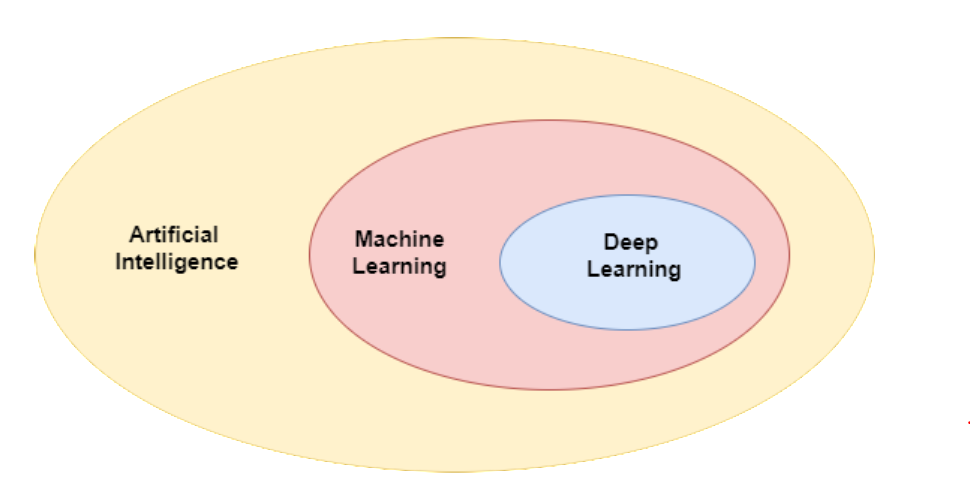
\includegraphics[scale=0.25]{./Figures/ai_ml_dl.png}
	\caption{Diferencias entre AI, ML y DL.}
	\label{fig:ai_ml_dl}
\end{figure}

\subsection{Inteligencia artificial}
Es un área de la computación que permite a los sistemas computacionales imitar la inteligencia humana para entender su entorno y tomar acciones que maximicen sus posibilidades de lograr sus objetivos \cite{ai_def}. Sus aplicaciones más importantes se encuentran en las áreas de comercio, educación, robótica, salud, agricultura, automotriz y finanzas\cite{ai_apps}. Todos los sistemas de inteligencia artificial reales e hipotéticos pueden ser clasificados en alguno de los siguientes tipos \cite{ai_types}:
\begin{itemize}
	\item Inteligencia artificial estrecha: también conocida como inteligencia artificial débil, su objetivo es llevar a cabo un solo tipo de tarea. Estos sistemas no poseen conciencia y no son manejados por sentimientos como lo haría un humano. Algunos ejemplos son los \textit{chatbots} o los automóviles autónomos.
	\item Inteligencia artificial general: también conocida como inteligencia artificial fuerte, es un concepto en el que las máquinas exhiben inteligencia humana. Estos sistemas tendrían la capacidad de aprender, entender y actuar de tal manera que sería indistinguible a un humano. Actualmente no existe, pero es utilizado conceptualmente en industrias como el cine.
	\item Super inteligencia artificial: también forma parte de la inteligencia artificial fuerte. Se le considera muy poderosa por ser capaz de volverse consciente y autónoma. No solo replica el comportamiento humano, sino que lo supera. Puede pensar mejor y tener más habilidades. Sin embargo, esta tecnología aún está en desarrollo.
\end{itemize}

\subsection{Aprendizaje automático}
Es un subconjunto de AI que utiliza algoritmos de aprendizaje estadísticos para construir sistemas con la habilidad de aprender automáticamente y mejorar a partir de experiencias previas sin ser explícitamente programados para esto \cite{ml_def}. Muchos de los servicios de recomendación empleados por empresas como Netflix, YouTube o Spotify, utilizan ML para adaptarse a un usuario en particular y ofrecer una mejor experiencia más personalizada \cite{ml_apps}. Estos algoritmos pueden ser clasificados de la siguiente manera \cite{ml_types}
\begin{itemize}
	\item Aprendizaje supervisado: se refiere al aprendizaje modelos a partir de un conjunto de datos, mejor conocidos como \textit{dataset}, cuyas respuestas son conocidas con antelación y están asociadas a una etiqueta o \textit{label}. Por ejemplo, el \textit{dataset} pueden ser muchas fotografías de gatos y el \textit{label} asociado el nombre de este animal. De esta manera el modelo es entrenado para generar predicciones de datos nuevos.
	
	\item Aprendizaje no supervisado: es usado cuando los datos utilizados para el aprendizaje no tienen \textit{labels}. Su objetivo principal es aprender acerca de los datos e inferir patrones sin ningún tipo de referencia sobre las respuestas esperadas. Es mayormente empleado como parte del análisis exploratorio de datos \cite{ai_ml_dl}.
	
	\item Aprendizaje reforzado: es el aprendizaje mediante la interacción continua con el entorno con el método de prueba y error, y utiliza continuamente la retroalimentación de sus acciones y experiencias previas. Este tipo de aprendizaje emplea recompensas si se realizan acciones correctas y penalizaciones si son incorrectas.
\end{itemize}

\subsection{Aprendizaje profundo}
Es una técnica de ML que está inspirada en la forma en la que el cerebro humano filtra información \cite{dl_def}. Cómo DL procesa información de manera similar al cerebro humano, sus aplicaciones son tareas que un humano generalmente realiza, como distinguir entre un peatón o un poste de luz en el caso de automóviles autónomos. El componente principal de DL son las redes neuronales artificiales, que son capas de nodos interconectados, donde existe una capa de entrada, una o varias capas ocultas y una capa de salida. En la figura \ref{fig:dl_nn} se puede observar la arquitectura de una red neuronal artificial.
\begin{figure}[h]
	\centering
	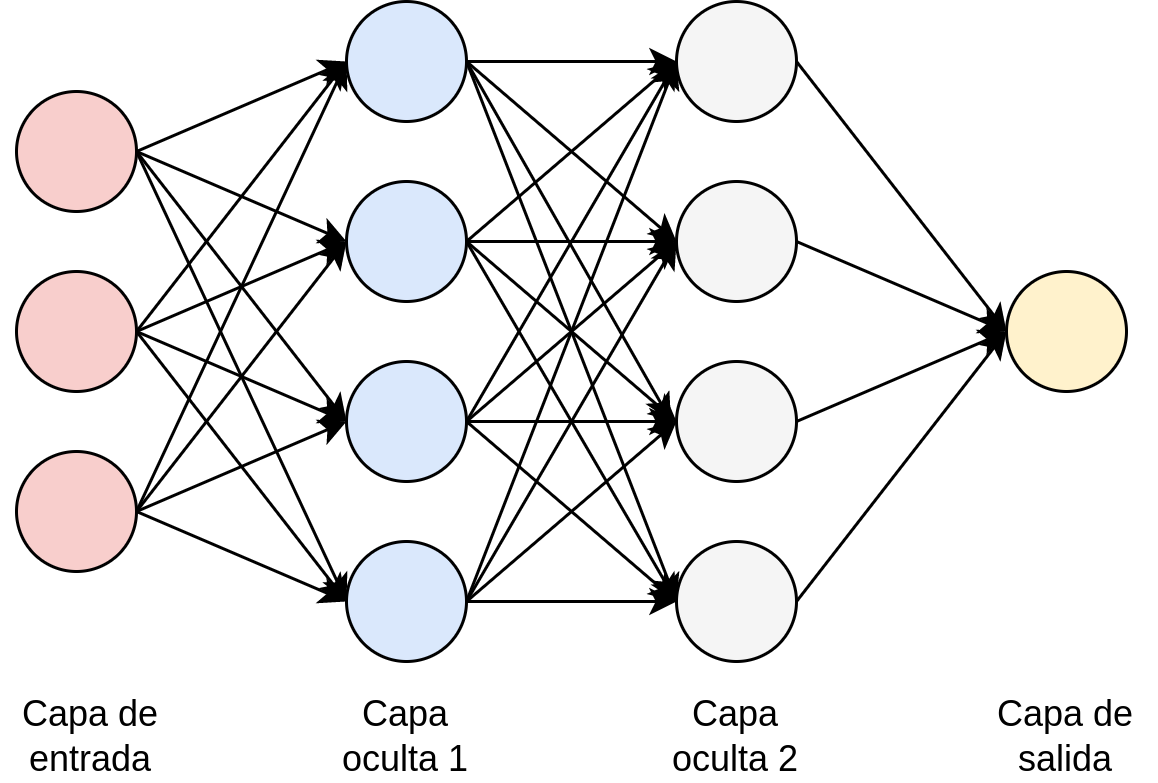
\includegraphics[scale=0.25]{./Figures/dl_nn.png}
	\caption{Arquitectura de una red neuronal artificial.}
	\label{fig:dl_nn}
\end{figure}


Cada uno de los nodos de las capas ocultas y de salida, tienen como entrada la salida de los nodos anteriores multiplicadas por unos términos denominados pesos o \textit{weights} y que sumados junto a otro término llamado sesgo o \textit{bias} pasan por una función de activación no lineal para generar su salida. En la figura \ref{fig:dl_node} se visualiza un nodo de las capas ocultas o de salida.
\begin{figure}[h]
	\centering
	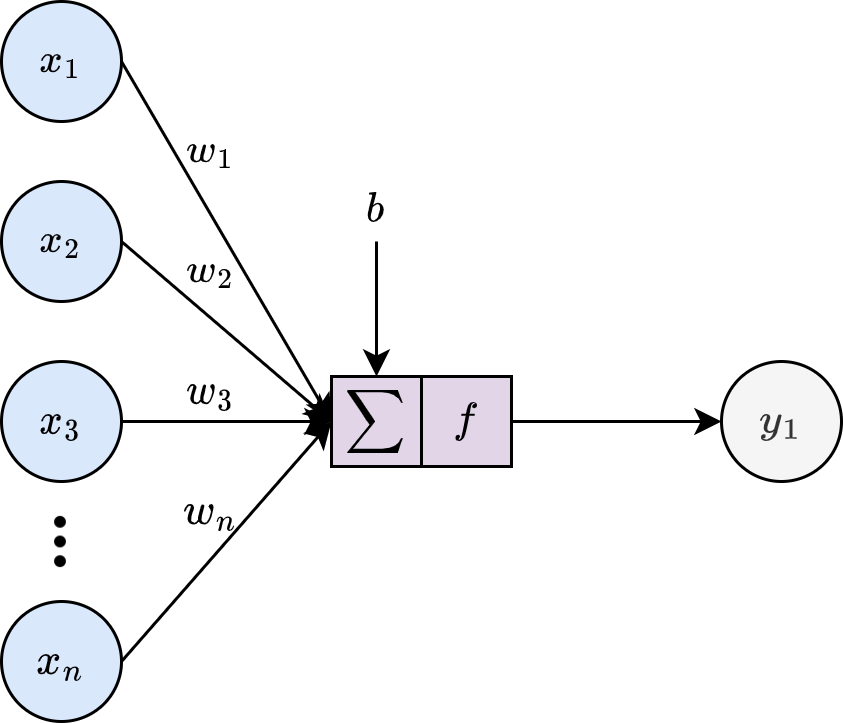
\includegraphics[scale=0.25]{./Figures/dl_node.png}
	\caption{Nodo de una red neuronal artificial.}
	\label{fig:dl_node}
\end{figure}

%----------------------------------------------------------------------------------------
\section{Redes neuronales convolucionales}
También conocidas como CNN (\textit{Convolutional Neural Networks}) por sus siglas en inglés, son un algoritmo de DL que están orientadas a recibir como entrada una imagen digitalizada, asignarle \textit{weights} y \textit{biases} entrenables a varios aspectos/objetos en la imagen para poder diferenciarlas unas de otras \cite{cnn_def}. Su uso reduce el preprocesamiento de las imágenes de entrada con respecto a otros modelos de clasificación, ya que los filtros necesarios son incorporados en su arquitectura y tienen la habilidad de ser entrenados.

Computacionalmente una imagen puede ser muy difícil de procesar, esto depende del espacio de colores donde se encuentra \cite{cnn_colors} y las dimensiones que posee. Por ejemplo, una imagen RGB y de dimensiones 1920x1080 píxeles tiene un tamaño de 6220800 bytes. El objetivo principal de las CNN es reducir la dimensionalidad de las imágenes de entrada, de tal forma que sean más fáciles de procesar y no pierdan sus características o \textit{features} principales que son críticas para obtener una buena predicción.

La arquitectura de una CNN es independiente del tipo de aplicación, donde las capas que lo componen son elegidas en función de los objetivos que se persiguen. En la figura \ref{fig:cnn_arch} se puede observar la arquitectura de una CNN para clasificar dígitos escritos a mano.

\begin{figure}[h]
	\centering
	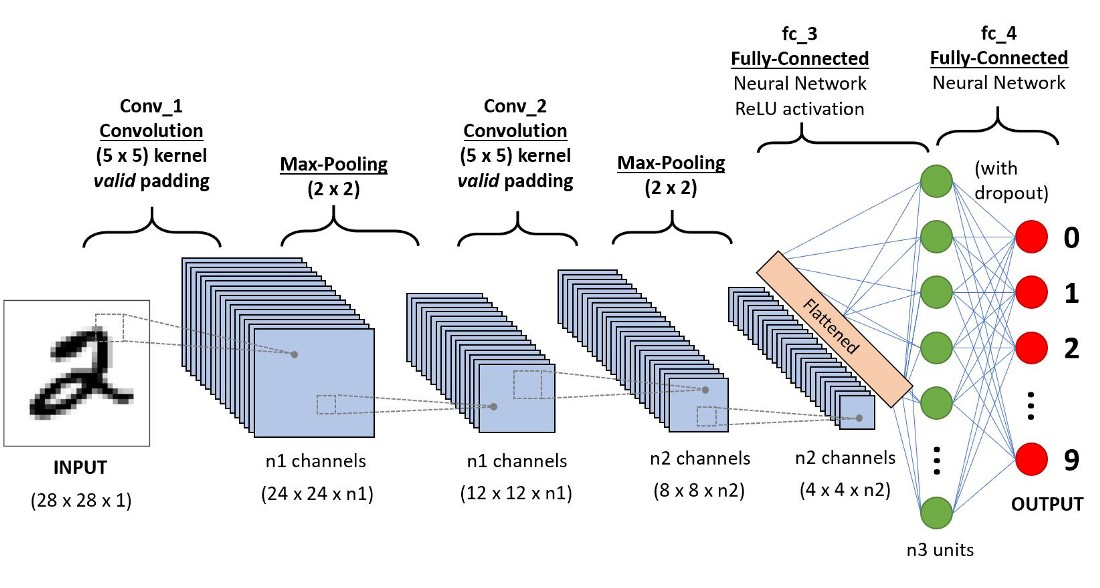
\includegraphics[scale=0.35]{./Figures/cnn_arch.jpeg}
	\caption{CNN para clasificar dígitos escritos a mano\protect\footnotemark.}
	\label{fig:cnn_arch}
\end{figure}
\footnotetext{Imagen tomada de: \url{https://towardsdatascience.com/a-comprehensive-guide-to-convolutional\\-neural-networks-the-eli5-way-3bd2b1164a53}}

En la arquitectura de la figura \ref{fig:cnn_arch} se pueden observar tres capas principales para construir una CNN: capa de convoluciones, capa de \textit{pooling} y capa \textit{fully-connected}.

\subsection{Capa de convoluciones}
Esta capa es la encargada de aplicar la operación de convolución sobre las imágenes de entrada para encontrar patrones que más adelante permitirán clasificarlas. La convolución de una imagen con un \textit{kernel} no es más que la aplicación del operador punto entre ambos. Este tipo de capas se definen por:
\begin{itemize}
	\item El número de los \textit{kernels} o filtros que se aplican a la imagen, que es el número de matrices por las que se van a convolucionar las imágenes de entrada.
	\item El tamaño de los \textit{kernels}, donde casi siempre tienen dimensiones cuadradas e impares como 3x3 o 5x5.
	\item El \textit{stride} o paso, se refiere a la forma en como el \textit{kernel} recorre la imagen.
\end{itemize}

En la figura \ref{fig:cnn_conv} se puede observar la operación de convolución de una entrada con dimensiones 3x3 y un \textit{kernel} de 2x2.

\begin{figure}[h]
	\centering
	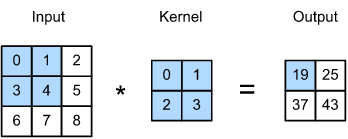
\includegraphics[scale=0.7]{./Figures/cnn_conv.png}
	\caption{Convolución de una entrada de 3x3 con un \textit{kernel} de 2x2 y \textit{stride} de 1\protect\footnotemark.}
	\label{fig:cnn_conv}
\end{figure}
\footnotetext{Imagen tomada de: \url{https://towardsdatascience.com/a-comprehensive-guide-to-convolutional\\-neural-networks-the-eli5-way-3bd2b1164a53}}

\subsection{Capa de \textit{pooling}}
Similar a la capa de convoluciones, tiene el objetivo de reducir la dimensionalidad de los \textit{features} obtenidos mediante las convoluciones aplicadas en la capa anterior, para reducir el poder computacional requerido en un principio. Existen dos tipos de dos tipos: \textit{max pooling} y \textit{Average pooling}. El primero retorna el valor máximo de una porción de la imagen cubierta por el \textit{kernel} y el segundo el valor promedio o \textit{average}. \textit{Max pooling} también funciona como supresor de ruido al mismo tiempo que reduce la dimensionalidad. Mientras que \textit{average pooling} solo sirve para reducir la dimensionalidad. En la figura \ref{fig:cnn_pool} se pueden observar estos tipos de \textit{pooling}.

\begin{figure}[h]
	\centering
	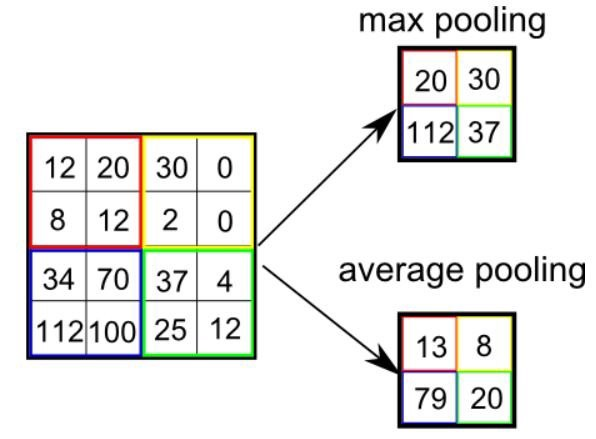
\includegraphics[scale=0.3]{./Figures/cnn_pool.png}
	\caption{Tipos de \textit{pooling}\protect\footnotemark.}
	\label{fig:cnn_pool}
\end{figure}
\footnotetext{Imagen tomada de: \url{https://towardsdatascience.com/a-comprehensive-guide-to-convolutional\\-neural-networks-the-eli5-way-3bd2b1164a53}}

\subsection{Capa \textit{fully-connected}}
También conocida como capa lineal o FC por sus siglas en inglés, es simplemente una red neuronal artificial como la mostrada en la sección anterior y se utiliza después de que las capas de convolución y \textit{pooling} desglosan los \textit{features} más importantes presentes en la imagen de entrada de la CNN. La capa FC brinda las probabilidades finales para cada \textit{label} esperado.

%----------------------------------------------------------------------------------------
\section{Vision artificial}
La visión artificial o \textit{computer vision} es un campo científico interdisciplinario que se encarga de cómo los sistemas computacionales pueden obtener un entendimiento de alto nivel de imágenes y videos digitales para comprender y automatizar tareas como lo haría un sistema de visión humano. Las tareas que ejecuta un sistema de visión artificial son de adquisición, procesamiento, análisis y entendimiento de imágenes. En la figura \ref{fig:mv_comp} se pueden apreciar las similitudes de un sistema de visión artificial y un sistema de visión humano.

\begin{figure}[h]
	\centering
	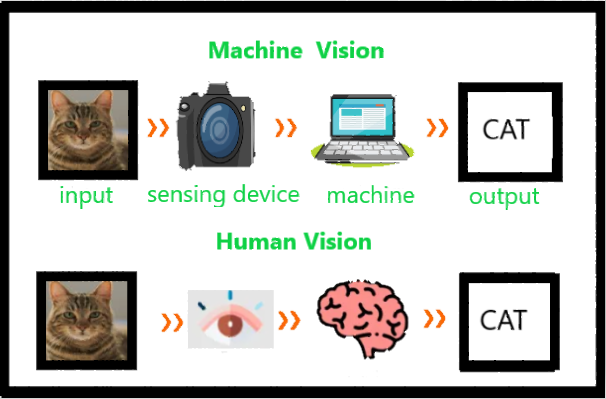
\includegraphics[scale=0.3]{./Figures/mv_comp.png}
	\caption{Componentes de un sistema de visión artificial y un sistema de visión humano.}
	\label{fig:mv_comp}
\end{figure}

Uno de los campos de estudio más importantes de la visión artificial es la detección facial. La detección facial puede ser considerada como un caso particular de la detección de objetos y tiene los objetivos de detectar y localizar todos los rostros humanos contenidos en una imagen digital. En la figura \ref{fig:mv_fd} se puede observar una imagen procesada por un sistema de detección facial.

\begin{figure}[h]
	\centering
	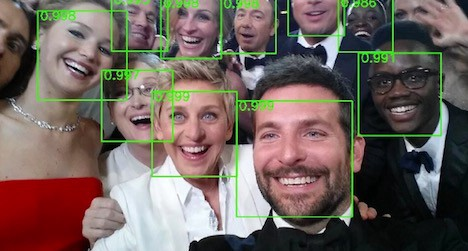
\includegraphics[scale=0.5]{./Figures/mv_fd.jpeg}
	\caption{Imagen procesada por un sistema de detección facial\protect\footnotemark.}
	\label{fig:mv_fd}
\end{figure}
\footnotetext{Imagen tomada de: \url{https://pbarasia.medium.com/use-face-recognition-on-whatsapp-group-\\pictures-part-1-832c6a74b5e5}}

Hoy en día, muchos dispositivos comerciales y profesionales como \textit{smartphones}, \textit{tablets} y robots, utilizan la detección facial como primer paso para otro tipo de aplicaciones más complejas, entre las que destacan: reconocimiento facial, computación afectiva y grabación de vídeo inteligente \cite{fd_apps}.

%----------------------------------------------------------------------------------------
\section{Servicios en la nube}
El término servicios en la nube hace referencia a un amplio rango de servicios ofrecidos bajo demanda a compañías y usuarios a través de internet. Estos servicios están diseñados para proveer de una manera fácil y asequible acceso a aplicaciones y recursos, sin la necesidad de una infraestructura o hardware propios \cite{cs_def}.

Los servicios en la nube son administrados totalmente por proveedores de computación en la nube o \textit{cloud computing} \cite{cs_def}. Estos se encuentran disponibles para los usuarios desde los servidores de los proveedores, por lo que no es necesario que una empresa aloje aplicaciones en sus propios servidores. De manera general, existen tres tipos básicos de servicios en la nube: Software como un servicio (SaaS, \textit{Software as a Service}), Infraestructura como un servicio (IaaS, \textit{Infrastructure as a Service}) y Plataforma como un servicio (PaaS, \textit{Platform as a Service}).

\subsection{Software como un servicio}
En este servicio el proveedor solo proporciona el software o aplicaciones en la nube mediante internet. Los clientes tienen acceso a través de interfaces de aplicación o a través de la web, que les permite interactuar de manera sencilla, sin la necesidad de gestionar, instalar ni actualizar el software.

\subsection{Infraestructura como un servicio}
Este servicio implica la contratación de una infraestructura de hardware a un tercero, donde varios clientes comparten los recursos de una máquina física. El proveedor proporciona a sus clientes el acceso a los recursos computacionales necesarios para almacenar o ejecutar tareas que pueden incluir servidores, redes, \textit{backup}, \textit{firewalls}, entre otros.

\subsection{Plataforma como un servicio}
Es un servicio que se encuentra conceptualmente entre SaaS e IaaS al eliminar la parte física de la infraestructura y ofrece una plataforma donde los clientes pueden crear, desarrollar, gestionar y distribuir sus aplicaciones. El proveedor es el encargado de la gestión y mantenimiento de la plataforma y permite que los clientes se dediquen exclusivamente al desarrollo.

%----------------------------------------------------------------------------------------
\section{Motivación}
Gracias a la amplia gama de plataformas de hardware y la disponibilidad de bibliotecas de código abierto para implementar AI, ML y DL, además de la difusión de información en foros y sitios web especializados, es posible desarrollar sistemas de visión artificial personalizados para distintos tipos de arquitecturas \cite{mot_emb}.

Normalmente las bibliotecas de código y los algoritmos para visión artificial no son aptos para dispostivos con poca cantidad de memoria y poder de computo reducido. Aunque gracias a los constantes avances en el desarrollo de herramientas para optmizar modelos de DL y arquitecturas de modelos mas eficientes y ligeras, es posible implementar estos algoritmos en dispositivos como microcontroladores.

La motivación principal de este trabajo fue desarrollar un sistema embebido de bajo costo económico, bajo consumo energético y de código abierto, que integre algoritmos de DL para visión artificial enfocados en cumplir eficientemente la tarea de detección facial.

Una motivación adicional fue integrar otra tecnología actual como es el internet de las cosas (IoT, \textit{Internet of Things}), para trabajar en conjunto con los algoritmos de visión artificial. Así las aplicaciones que se pueden obtener son más versátiles a la hora de su implementación en entornos urbanos.

%----------------------------------------------------------------------------------------
\section{Estado del arte}
Como antecedente existe el trabajo de Ilhan Aydin y Nashwan Adnan Othman, denominado ``A new IoT combined face detection of people by using computer vision for security application`` \cite{soa_ref}. El \textit{paper} donde se describe su trabajo presenta el desarrollo de un dispositivo electrónico que tiene como componentes principales una Raspberry Pi 3, un sensor pasivo infrarrojo (PIR, \textit{Passive Infra Red}) y una cámara. Su objetivo principal es detectar personas con ayuda del sensor de movimiento PIR, fotografiarlas y aplicar el algoritmo de detección facial Haar Cascade \cite{haar_cascade}, para posteriormente guardar una imagen del rostro detectado y visualizarla en un teléfono móvil con ayuda de la aplicación Telegram. En la figura \ref{fig:soa_arch} se puede observar el diagrama en bloques del sistema descrito anteriormente.

\begin{figure}[h]
	\centering
	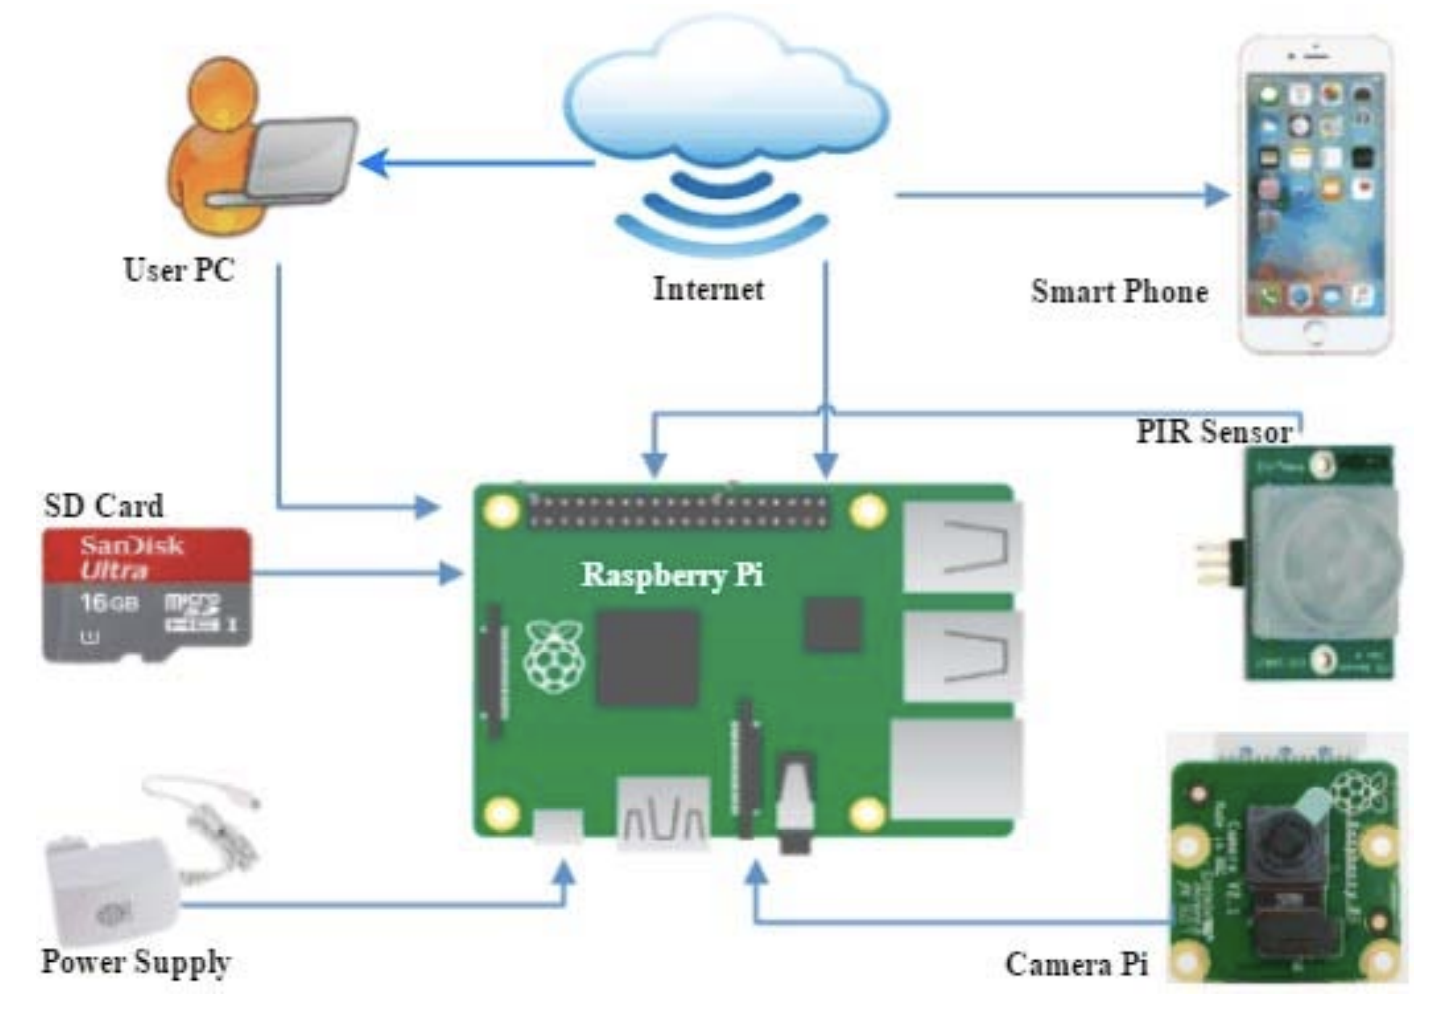
\includegraphics[scale=0.4]{./Figures/soa_arch.png}
	\caption{Diagrama en bloques del sistema propuesto en \cite{soa_ref}}
	\label{fig:soa_arch}
\end{figure}

%----------------------------------------------------------------------------------------
\section{Objetivos y alcance}
El objetivo principal de este trabajo fue desarrollar un sistema embebido con la capacidad de ejecutar modelos de AI para detectar y localizar rostros humanos de imágenes digitales capturadas por su cámara.

El alcance de este trabajo incluyó:
\begin{itemize}
	\item Contruir un prototipo de pruebas
	\item Desarrollar e implementar los modelos de AI necesarios
	\item Implementar los servicios en la nube necesarios
\end{itemize}
%----------------------------------------------------------------------------------------
\section{Requerimientos}
Los requerimientos planteados para este trabajo fueron:
\begin{enumerate}
	\item Requerimientos funcionales
  \begin{enumerate}
     	\item El sistema debe detectar y contar todos los rostros existentes de las imágenes obtenidas por su cámara con ayuda de las técnicas de procesamiento de imágenes \textit{pyramid image} y \textit{slidding window}, y modelos de DL que alcancen una precisión de al menos 80\%.
		\item El sistema debe conectarse a una red Wi-Fi existente a través de algún mecanismo de aprovisionamiento de credenciales de red.
		\item El sistema debe establecer comunicación con los servidores de AWS.
		\item El sistema debe ser alimentado mediante dos baterías AA de litio.
		\item El sistema debe poseer mecanismos de seguridad implementados tanto en hardware como en firmware para evitar su manipulación incorrecta.
		\item El sistema debe funcionar solamente si se detecta movimiento en el sector donde se encuentra instalado.
	\end{enumerate}
	\item Requerimientos no funcionales
	\begin{enumerate}
		\item El sistema debe tener un costo de desarrollo igual o menor a US\$200.
		\item El sistema debe tener documentación adecuada sobre su uso y desarrollo.
	\end{enumerate}
\end{enumerate}



%----------------------------------------------------------------------------------------





\chapter{Introducción específica} % Main chapter title

\label{Chapter2} % Change X to a consecutive number; for referencing this chapter elsewhere, use \ref{ChapterX}

%----------------------------------------------------------------------------------------
Este capítulo expone una descripción detallada del sistema, del hardware utilizado y las herramientas de  software necesarias en el desarrollo del trabajo. Se abarcan la descripción del sistema y sus componentes, los \textit{frameworks} y modelos utilizados para detección facial y las herramientas utilizadas en la web.

%----------------------------------------------------------------------------------------
\section{Funcionamiento general del sistema}
Este capítulo expone una descripción detallada del sistema, del hardware utilizado y las herramientas de software necesarias en el desarrollo del trabajo. Se abarcan la descripción del sistema y sus componentes, los \textit{frameworks} y modelos empleados para detección facial y las herramientas utilizadas en la web.

\begin{figure}[h]
	\centering
	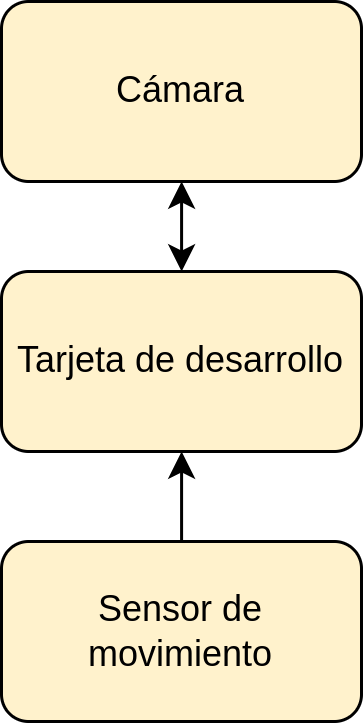
\includegraphics[scale=0.25]{./Figures/sys_blocks.png}
	\caption{Diagrama en bloques del sistema.}
	\label{fig:sys_blocks}
\end{figure}

En el sistema de la figura \ref{fig:sys_blocks}, cuando el sensor de movimiento detecta el movimiento de una persona genera una señal que notifica a la tarjeta de desarrollo sobre este evento. Entonces la tarjeta de desarrollo activa la cámara y obtiene una fotografía para procesarla. La imagen digital obtenida es procesada y utilizada como entrada para los modelos de DL. Cuando se obtienen las inferencias deseadas de los modelos, los resultados son procesados para transmitirlos hacia los servidores en la nube encargados de procesarlos y mostrarlos a los usuarios finales.

\subsection{Tarjeta de desarrollo}
El componente central del sistema es la tarjeta de desarrollo ESP32-S3-DevKitC-1-N8R8 de la empresa Espressif. Tiene como componente central el módulo ESP32-S3-WROOM-1-N8R8 basado en el sistema en chip (SoC, \textit{Systems on Chip}) ESP32-S3 y varios otros componentes que simplifican el proceso de desarrollo de aplicaciones para IoT. En la figura \ref{fig:devkit_comp} se observa una fotografía de la tarjeta con el detalle de sus componentes.

\begin{figure}[h]
	\centering
	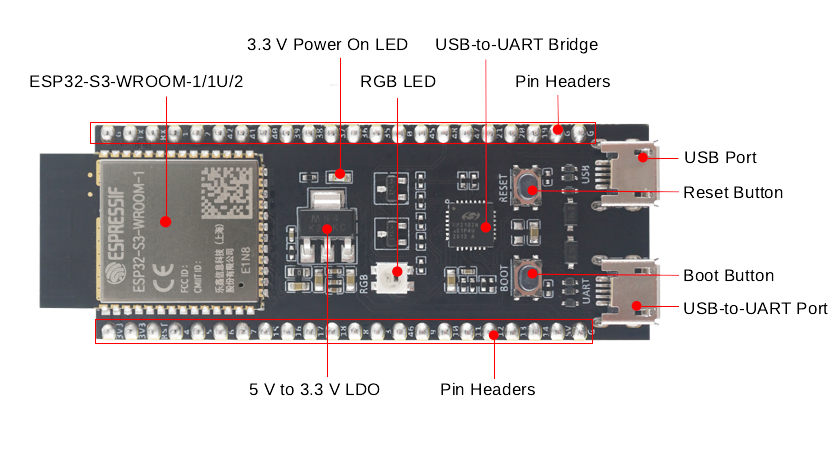
\includegraphics[scale=0.45]{./Figures/devkit_comp.png}
	\caption{Componentes del ESP32-S3-DevKitC-1\protect\footnotemark.}
	\label{fig:devkit_comp}
\end{figure}
\footnotetext{Imagen tomada de: \url{https://docs.espressif.com/projects/esp-idf/en/latest/esp32s3/hw-reference/esp32s3/user-guide-devkitc-1.html}}

El módulo ESP32-S3-WROOM-1-N8R8 es un potente módulo que incorpora un microcontrolador (MCU, \textit{Microcontroller Unit}) de doble núcleo con conectividad Wi-Fi y Bluetooth de baja energía (BLE, \textit{Bluetooth Low Energy}), además posee un amplio conjunto de periféricos. Sus especificaciones técnicas más relevantes se detallan en la tabla \ref{tab:devkit_specs}.

\begin{table}[h]
	\centering
	\caption[ESP32-S3-DevKitC-1 especificaciones]{Tabla de especificaciones del ESP32-S3-DevKitC-1 \cite{devkit_info}.}
	\begin{tabular}{lc}   
		\toprule
		\textbf{Característica} 	 & \textbf{Descripción}  \\
		\midrule
		SoC embebido & ESP32-S3R8 \\
		Procesador & Xtensa LX7 doble núcleo de 32 bits \\
		Frecuencia & Hasta 240 MHz \\
		ROM & 384 KB \\
		SRAM & 512 KB \\
		Pines & 41 \\
		Flash & 8 MB \\
		PSRAM & 8 MB \\
		Tipo de antena & PCB \\
		Wi-Fi & 802.11 b/g/n hasta 150 Mbps \\
		Bluetooth & Bluetooth 5 y Bluetooth \textit{mesh} \\
		Periféricos & \begin{tabular}{@{}c@{}} GPIO, I2C, SPI, interfaz LCD, \\ interfaz de cámara, UART, I2S, USB, PWM, ADC, \\ sensor táctil, sensor de temperatura, timer y \textit{watchdogs} \end{tabular} \\
	 	Rango de temperatura &  –40 \textcelsius\ a 65 \textcelsius \\
		\bottomrule
		\hline
	\end{tabular}
	\label{tab:devkit_specs}
\end{table}

En el mercado existen muchos fabricantes que ofrecen tarjetas de desarrollo de características técnicas que podrían haber sido utilizadas para el desarrollo de este trabajo. Sin ir muy lejos, Espressif, fabricante de la ESP32-S3-DevKitC-1-N8R8, tiene toda una familia de módulos y tarjetas muy similares entre sí. La elección de esta tarjeta en particular responde a los siguientes criterios:
\begin{itemize}
	\item Costo: Espressif ofrece en todos sus SoCs, módulos y tarjetas de desarrollo un costo muy contenido por la gran cantidad de características ofrecidas.
	\item Redes neuronales: la serie de SoCs ESP32-S3 ofrece soporte para instrucciones vectoriales, que acelera las tareas de computación de redes neuronales. Esta fue la característica más importante al momento de la elección de esta tarjeta.
	\item Memoria: como el trabajo implicaba el uso de una cámara y, por tanto, el manejo de \textit{buffers} de memoria de gran tamaño para manipular las imágenes obtenidas, la cantidad de memoria externa que ofrece esta tarjeta la hizo óptima para la aplicación.
\end{itemize}

\subsection{Sensor de movimiento}
Un sensor de movimiento PIR basa su funcionamiento al detectar diferencias en la energía IR (\textit{Infrared}, Infrarrojo) en el campo de visión del sensor. Debido a que la señal de salida generada por el sensor es muy pequeña, es necesario aplicar etapas de amplificación y filtrado para elevar el nivel de tensión de la señal de salida y al mismo tiempo filtrar el ruido que puede generar eventos falsos positivos. Esta salida analógica luego se debe convertir en una señal digital mediante la operación de comparación de ventanas y se puede utilizar, por ejemplo, como una interrupción en un MCU. En la figura \ref{fig:move_blocks} se muestra el diagrama en bloques del sensor de movimiento PIR.

\begin{figure}[h]
	\centering
	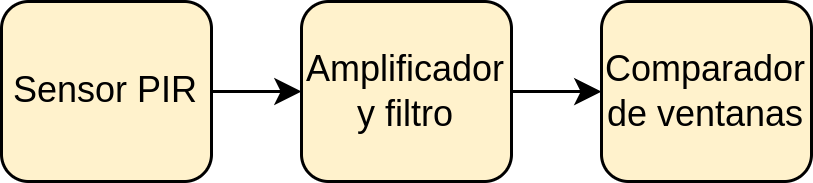
\includegraphics[scale=0.25]{./Figures/move_blocks.png}
	\caption{Diagrama en bloques del sensor de movimiento PIR.}
	\label{fig:move_blocks}
\end{figure}

\subsubsection{Sensor pasivo infrarojo}
El IRA-S230ST01 es un sensor PIR fabricado por la empresa Murata. Posee una alta sensibilidad y un rendimiento confiable gracias a la tecnología cerámica y la técnica de IC (\textit{Integrated Circuit}, Circuito Integrado) híbrida de Murata. Tiene además una sensibilidad mejorada a la interferencia de RF (\textit{Radio Frequency}, Radiofrecuencia). Sus aplicaciones más comunes incluyen sistemas de seguridad, aparatos de iluminación, electrodomésticos, entre otros \cite{pir_info}. En la figura \ref{fig:pir_photo} se puede observar una fotografía del IRA-S230ST01.

\vspace*{60 px}

\begin{figure}[h]
	\centering
	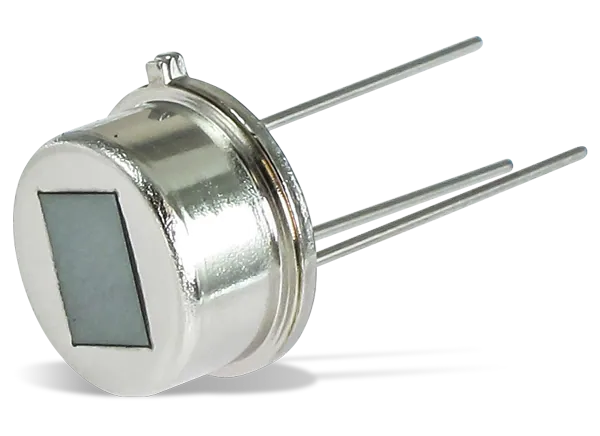
\includegraphics[scale=0.2]{./Figures/pir_photo.png}
	\caption{Fotografía del sensor IRA-S230ST01\protect\footnotemark.}
	\label{fig:pir_photo}
\end{figure}
\footnotetext{Imagen tomada de: \url{https://www.murata.com/en-sg/products/productdetail?partno=IRA-S230ST01}}

En la tabla \ref{tab:pir_specs} se detallan sus características técnicas más importantes.

\begin{table}[h]
	\centering
	\caption[IRA-S230ST01 especificaciones]{Tabla de especificaciones del IRA-S230ST01 \cite{pir_info}.}
	\begin{tabular}{lc}   
		\toprule
		\textbf{Característica} 	 & \textbf{Descripción}  \\
		\midrule
		Rango de temperatura & -40 \textcelsius\ a 70 \textcelsius\\
		SNR & 40 dB \\
		Campo de visión & theta1=theta2=45 grados \\
		Electrodo & (2.0x1.0mm)x2 \\
		Responsividad & 4.6 mV \\
		Filtro óptico & 5 \textmu m paso alto \\
		Fuente de alimentación & 2 V a 15 V \\
		\bottomrule
		\hline
	\end{tabular}
	\label{tab:pir_specs}
\end{table}

La elección del IRA-S230ST01 como sensor PIR responde a los siguientes criterios: \\
\begin{itemize}
	\item Marca: Murata es una marca muy reconocida en el mundo de los semiconductores y ofrece productos de muy alta calidad.
	\item Documentación: el IRA-S230ST01 cuenta con documentación muy clara sobre sus características técnicas.
\end{itemize}

\subsubsection{Amplificador operacional}
El TLV8544 es un amplificador operacional cuádruple de ultra bajo consumo de la empresa Texas Instruments, de costo optimizado para aplicaciones de detección en equipos inalámbricos y cableados de bajo consumo. El diseño del TLV8544 minimiza el consumo en dispositivos como sensores de movimiento para sistemas de seguridad, donde el tiempo de vida de la batería que los alimenta es crítico. Su uso más común es en configuraciones de amplificadores de transimpedancia con resistencias de \textit{feedback} en el orden de los Mega ohms. Adicionalmente, tiene protección contra EMI (\textit{Electromagnetic Interference}, Interferencia Electromagnética) que reduce la sensibilidad a las señales de RF no deseadas de fuentes como teléfonos móviles, Wi-Fi y transmisores de radio \cite{opamp_info}. En la figura \ref{fig:opamp_photo} se puede observar una fotografía del TLV8544 en un encapsulado TSSOP-14.

\vspace*{50 px}

\begin{figure}[h]
	\centering
	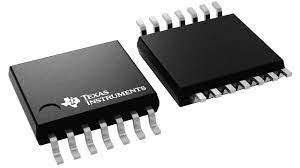
\includegraphics[scale=0.4]{./Figures/opamp_photo.jpeg}
	\caption{Fotografía del TLV8544 en un encapsulado TSSOP-14\protect\footnotemark.}
	\label{fig:opamp_photo}
\end{figure}
\footnotetext{Imagen tomada de: \url{https://www.ti.com/product/TLV8544}}

Las características técnicas más importantes del TLV8544 se presentan en la tabla \ref{tab:opamp_specs}.

\begin{table}[h]
	\centering
	\caption[TLV8544 especificaciones]{Tabla de especificaciones del TLV8544 \cite{opamp_info}.}
	\begin{tabular}{lc}   
		\toprule
		\textbf{Característica} 	 & \textbf{Descripción}  \\
		\midrule
		Número de canales & 4 \\
		Fuente de alimentación & 1,7 V a 3,6 V \\
		Corriente de salida por canal & 30 mA \\
		Corriente de operación & 500 nA \\
		CMMR (\textit{Common Mode Rejection Ratio}, \\ Relación de Rechazo del Modo Común) & 90 dB \\
		Rango de temperatura & -40 \textcelsius  a 125 \textcelsius\\
		Corriente de polarización & 100 fA \\
		Ancho de banda de ganancia & 8 kHz \\
		\bottomrule
		\hline
	\end{tabular}
	\label{tab:opamp_specs}
\end{table}

Desde hace muchos años los amplificadores operacionales son dispositivos muy utilizados por su gran cantidad de aplicaciones, en el mercado existen una gran variedad de modelos y son fabricados por muchas empresas de semiconductores. Estos fueron los criterios de elección del TLV8544 para el presente trabajo:
\begin{itemize}
	\item Aplicación: por sus características técnicas, el TLV8544 está diseñado para ser parte de las etapas de amplificación y filtrado en el diseño de un sensor de movimiento PIR.
	\item Documentación: Texas Instruments, además del correspondiente \textit{datasheet} del TLV8544, ofrece varios documentos técnicos con ejemplos de diseño para el TLV8544.
	\item Costo: es un dispositivo de precio muy razonable por todas las características que ofrece.
	\item Consumo energético: con sus 500 nA de corriente de funcionamiento por canal, el TLV8544 es una opción ideal para aplicaciones que requieran el uso de baterías.
\end{itemize}

\subsection{Cámara}
Otro de los componentes principales del sistema es la cámara, que permite obtener imágenes en un formato digital que posteriormente deben ser procesadas por los algoritmos de DL. Para este trabajo se utilizó el módulo ESP-LyraP-CAM. Este módulo integra un CCM (\textit{Compact Camera Module}, Módulo de Cámara Compacto) con un sensor OV2640 en conjunto con dos reguladores de tensión para su correcto funcionamiento. En la figura \ref{fig:camera_comp} se puede observar unas fotografías del módulo ESP-LyraP-CAM y sus componentes.

\begin{figure}[h]
	\centering
	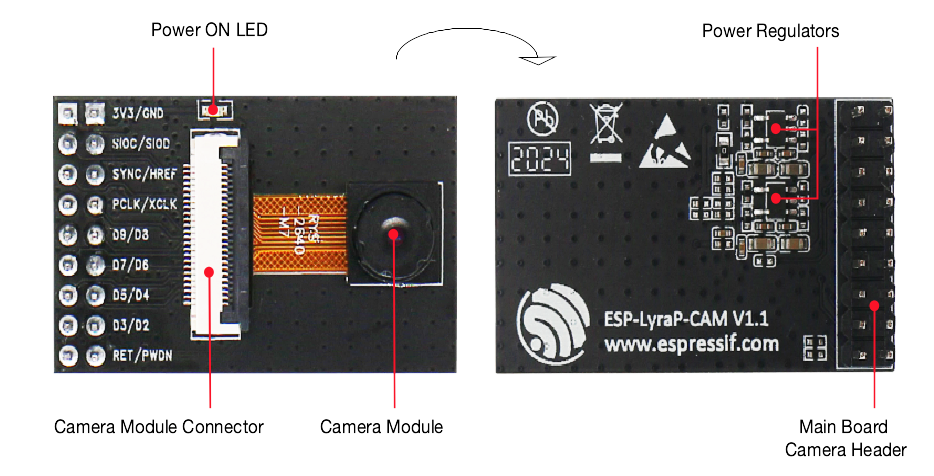
\includegraphics[scale=0.6]{./Figures/camera_blocks.png}
	\caption{Componentes del módulo ESP-LyraP-CAM\protect\footnotemark.}
	\label{fig:camera_comp}
\end{figure}
\footnotetext{Imagen tomada de: \url{https://docs.espressif.com/projects/esp-idf/en/latest/esp32s2/hw-reference/esp32s2/user-guide-esp-lyrap-cam-v1.1.html}}

El OV2640 de la empresa OmniVision es un sensor semiconductor de óxido metal complementario (CMOS, (\textit{Complementary Metal-Oxide-Semiconductor}) de 2 MP, cuenta con una interfaz de comunicación compatible con DVP  (\textit{Digital Video Port}, Puerto de Video Digital), soporta codificación JPEG y es de bajo consumo energético. En la tabla \ref{tab:ov2640_specs} se muestran las características técnicas más importantes del OV2640.

\begin{table}[h]
	\centering
	\caption[OV2640 especificaciones]{Tabla de especificaciones del OV2640 \cite{camera_info}.}
	\begin{tabular}{lc}   
		\toprule
		\textbf{Característica} 	 & \textbf{Descripción}  \\
		\midrule
		Tamaño de matriz & 1600x1200 (UXGA) \\		
		Fuente de alimentación & \begin{tabular}{@{}c@{}} \textit{Core}: 1.3 V ± 5\% \\ \textit{Analog} 2.5 ~ 3.0 V \\ I/O: 1,7 V - 3,3 V\end{tabular} \\
		Consumo energético & \begin{tabular}{@{}c@{}} \textit{Free running}: 125 mW \\ \textit{Standby}: 600 \textmu A \end{tabular} \\
		Formato de imagen del sensor & 1/4'' \\
		Tasa de transferencia maxima & \begin{tabular}{@{}c@{}} 1600×1200 a 15 fps \\ SVGA a 30 fps \\ CIF a 60 fps \end{tabular} \\
		Sensibilidad & 0.6 / Lux-sec \\
		SNR & 40 dB \\
		Rango dinámico & 50 dB \\
		Tamano de pixel & 2,2x2,2 \textmu m \\
		Formato de salida & YUV/RGB/MJPEG \\
		\bottomrule
		\hline
	\end{tabular}
	\label{tab:ov2640_specs}
\end{table}

Los criterios para utilizar este módulo como cámara del sistema son los siguientes:
\begin{itemize}
	\item Costo: los módulos con el sensor OV2640 tienen un costo muy reducido en comparación con otros disponibles en el mercado.
	\item Bajo consumo energético: como se mostró en la tabla \ref{tab:ov2640_specs} el consumo energético del módulo en modo \textit{standby} es lo suficientemente bajo como para funcionar alimentado por baterías.
	\item Disponibilidad de código: al ser un módulo que ya lleva mucho tiempo en el mercado existen muchas bibliotecas de código para utilizarlo, lo que simplifica en gran medida el tiempo de desarrollo de \textit{firmware}.
\end{itemize}

%----------------------------------------------------------------------------------------
\section{Redes Convolucionales en Cascada Multitarea}
Las redes convolucionales en cascada multitarea (MTCNN, \textit{Multi-task Cascaded Convolutional Networks}) son un \textit{framework} basado en el \textit{paper} \cite{mtcnn_info}, están desarrolladas para integrar las tareas de detección facial y alineamiento facial con ayuda de CNNs en cascada mediante aprendizaje multitarea. El proceso consta de tres etapas de CNNs que puede detectar rostros humanos, sus posiciones y las posiciones de sus rasgos faciales (nariz, ojos y boca). En la figura \ref{fig:mtcnn_pipe} se muestra el \textit{pipeline} utilizado en MTCNN.

\begin{figure}[h]
	\centering
	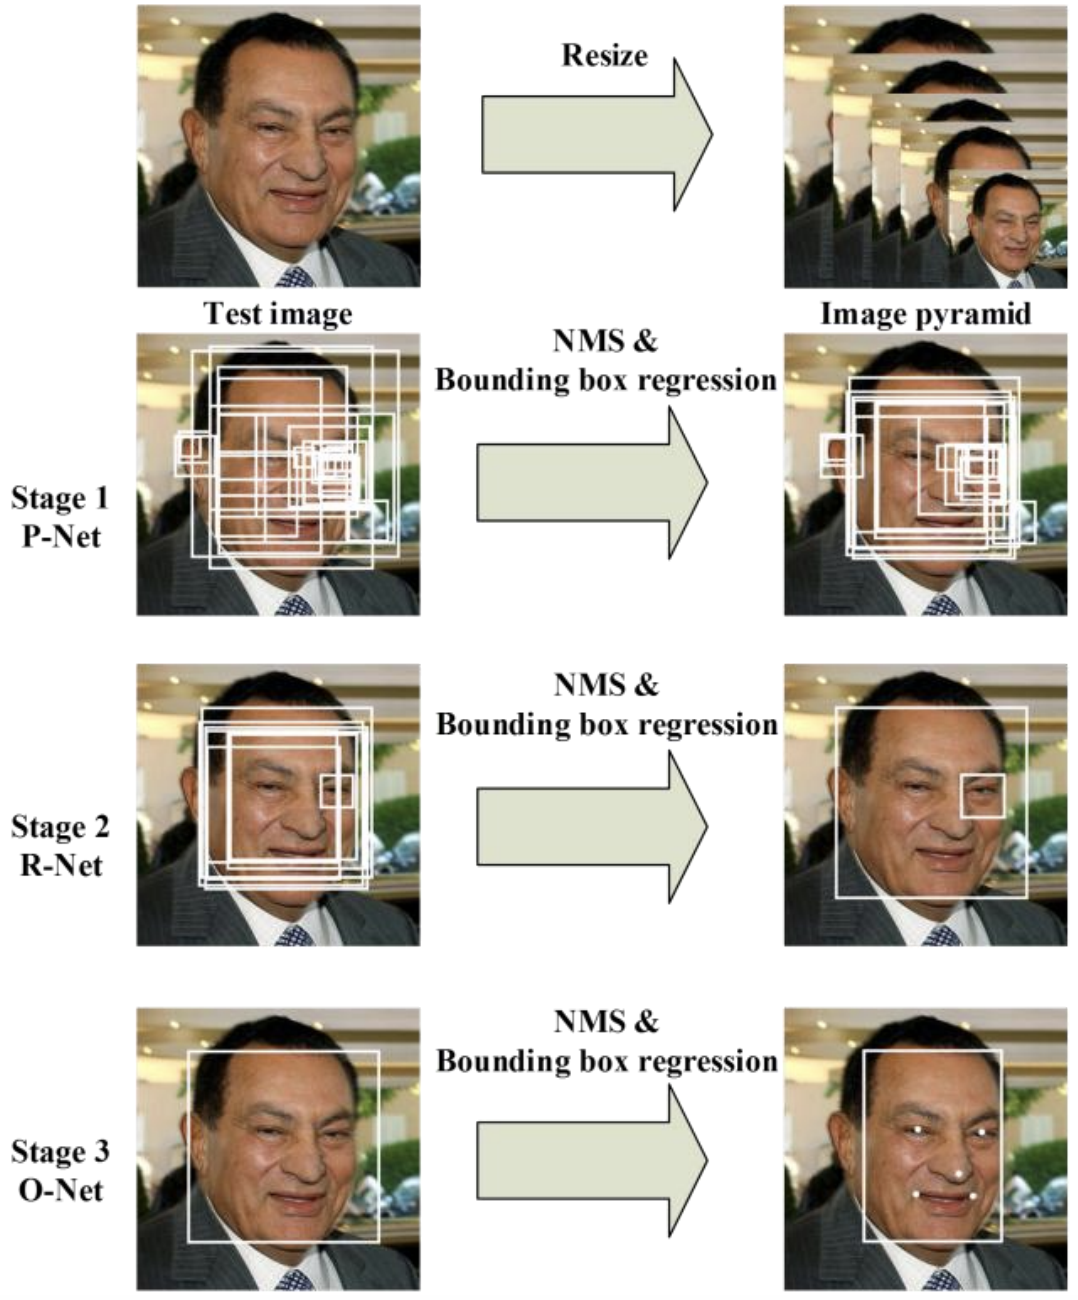
\includegraphics[scale=0.5]{./Figures/mtcnn_pipe.png}
	\caption{\textit{Pipeline} de MTCNN \cite{mtcnn_info}.}
	\label{fig:mtcnn_pipe}
\end{figure}

\subsection{Red de propuestas}
También conocida como P-Net (\textit{Proposal Network}), esta etapa está compuesta de una red totalmente convolucional (FCN, \textit{Fully Convolutional Network}). La diferencia entre una FCN y una CNN es que la FCN no utiliza una capa FC como parte de su arquitectura. Tiene la función de obtener ventanas candidatas y sus vectores de regresión de \textit{bounding box} a partir de varias escalas de la imagen original. La regresión de \textit{bounding box} es una técnica para predecir la localización de un cuadro delimitador en el que se encuentra el objeto que quiere ser detectado, en este caso rostros humanos. Una vez que se obtienen estos vectores, se realiza una operación conocida como NMS (\textit{Non Max Suppression}, Supresión no Máxima) para combinar las regiones superpuestas entre sí. Finalmente, las ventanas candidatas resultantes pasan a la siguiente etapa. En la figura \ref{fig:mtcnn_pnet} se muestra la arquitectura de P-Net.

\begin{figure}[h]
	\centering
	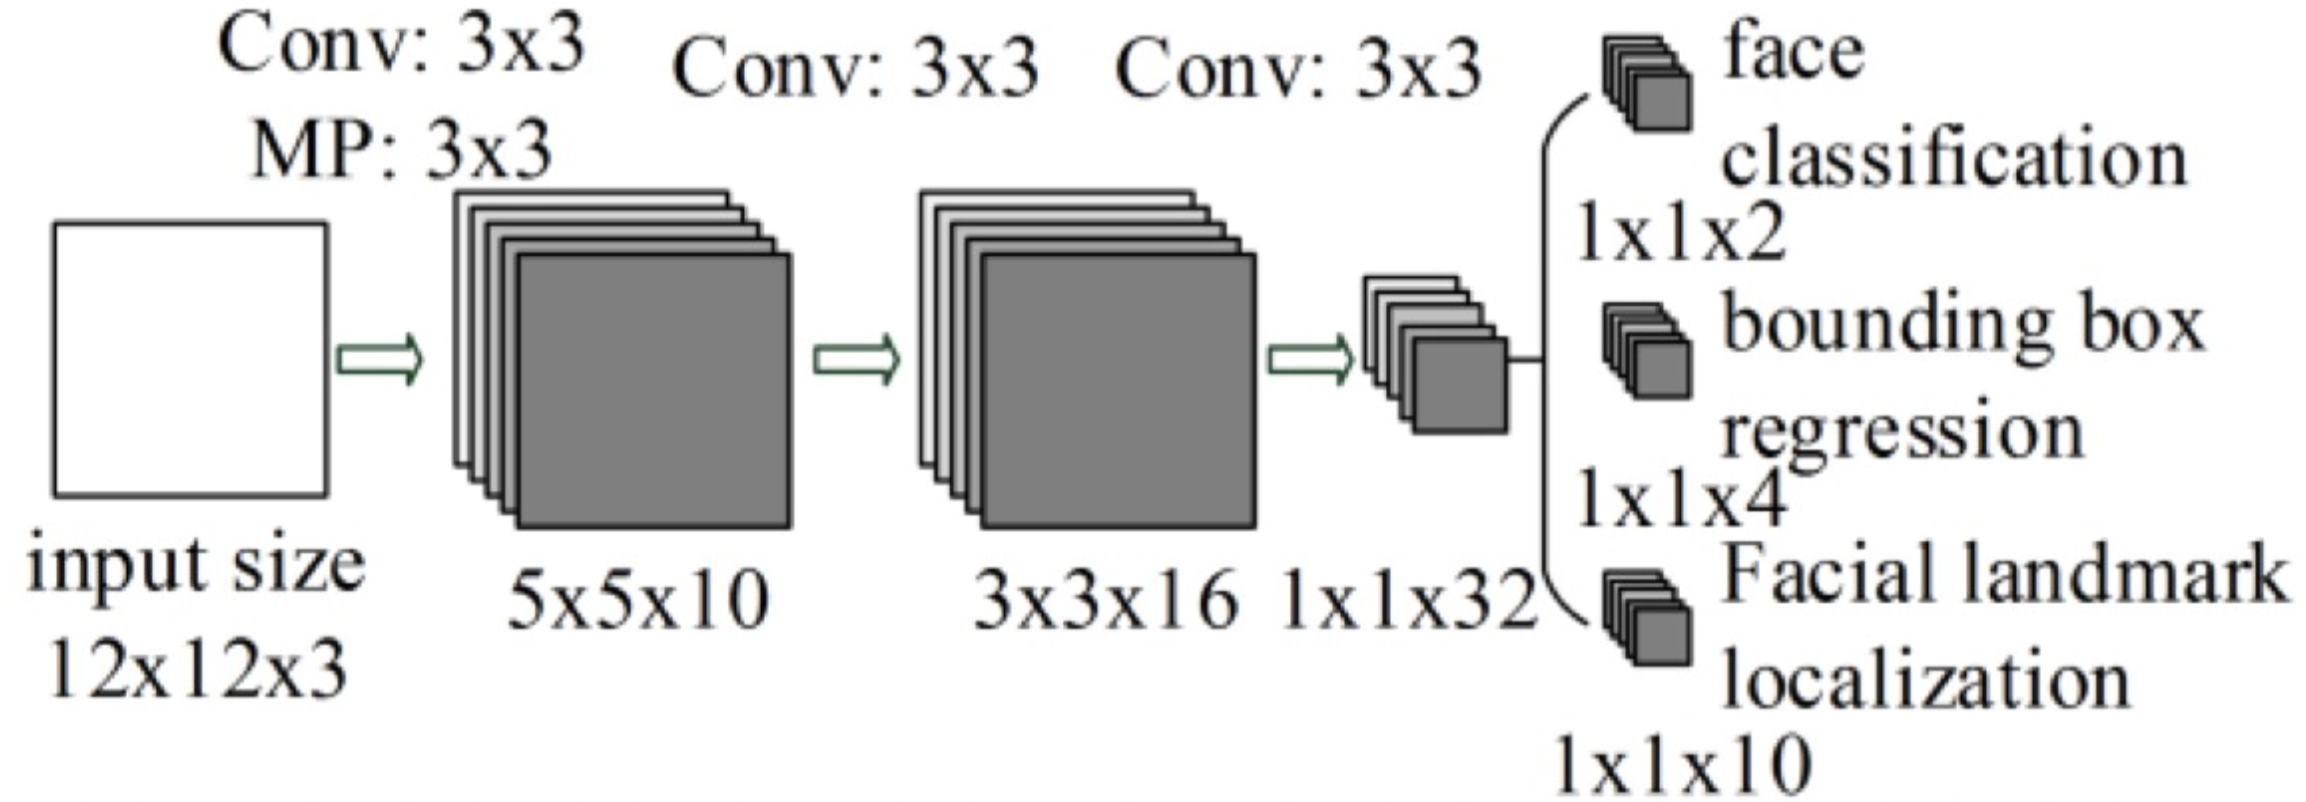
\includegraphics[scale=0.25]{./Figures/mtcnn_pnet.png}
	\caption{Arquitectura de P-Net \cite{mtcnn_info}.}
	\label{fig:mtcnn_pnet}
\end{figure}
	
\subsection{Red de refinamiento}
Esta es una CNN denominada R-Net (\textit{Refine Network}). Los candidatos provenientes de P-Net son la entrada de esta red. La arquitectura de R-Net reduce aún más el número de candidatos, realiza la calibración con regresión de \textit{bounding box} y emplea NMS para fusionar candidatos superpuestos. Para cada candidato de entrada, R-Net obtiene la probabilidad de si es un rostro o no, un vector de 4 elementos que es el \textit{bounding box} y un vector de 10 elementos que representan la localización de rasgos faciales. En la figura \ref{fig:mtcnn_rnet} se muestra la arquitectura de R-Net.

\begin{figure}[h]
	\centering
	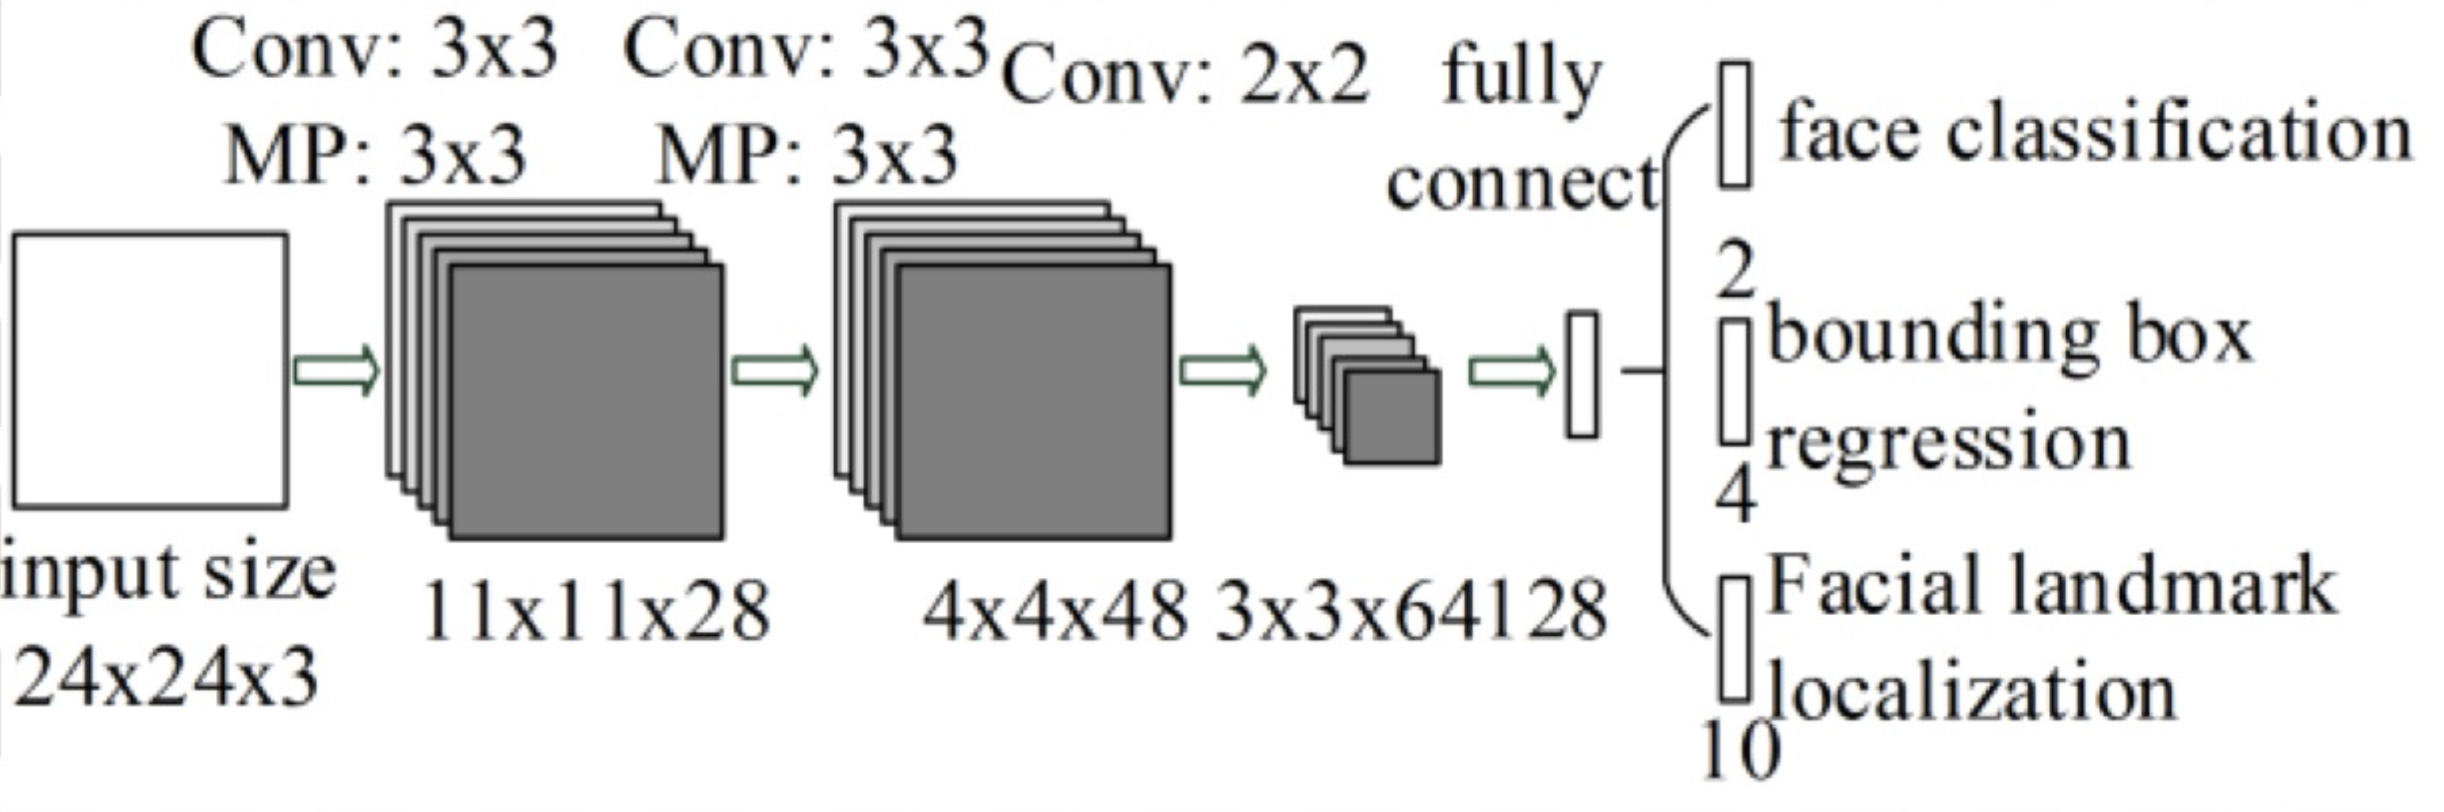
\includegraphics[scale=0.25]{./Figures/mtcnn_rnet.png}
	\caption{Arquitectura de R-Net \cite{mtcnn_info}.}
	\label{fig:mtcnn_rnet}
\end{figure}

\subsection{Red de salida}
Conocida como O-Net (\textit{Output Network}), es muy similar a R-Net, pero está enfocada a describir el rostro con más detalle y generar las cinco localizaciones para ojos, boca y nariz. Su arquitectura se muestra en la figura \ref{fig:mtcnn_onet}.

\begin{figure}[h]
	\centering
	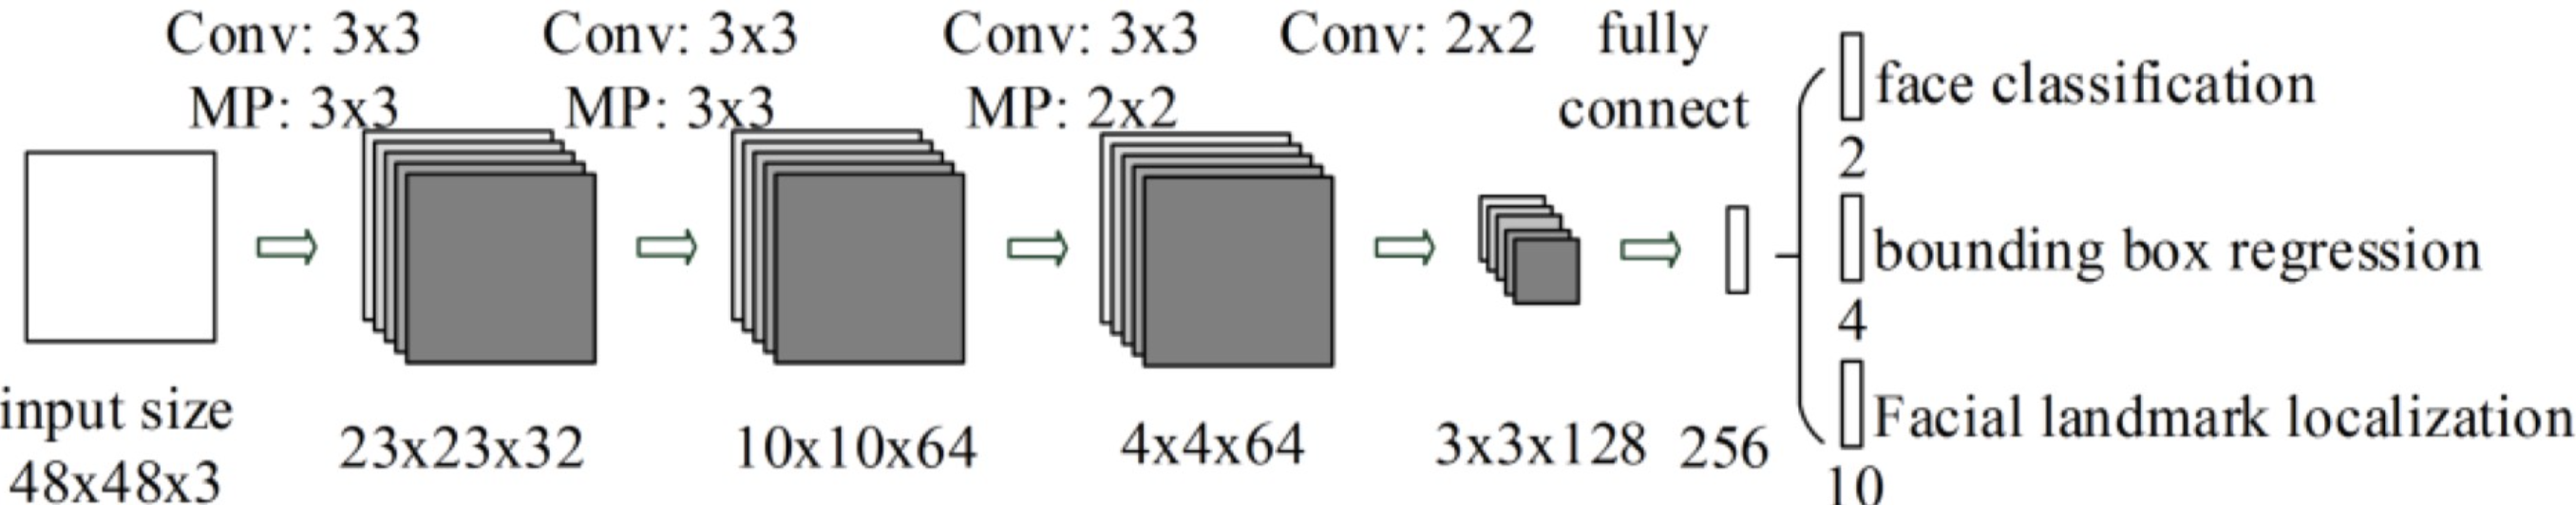
\includegraphics[scale=0.3]{./Figures/mtcnn_onet.png}
	\caption{Arquitectura de O-Net \cite{mtcnn_info}.}
	\label{fig:mtcnn_onet}
\end{figure}

\subsection{Tareas}
Como se explicó en los puntos anteriores, MTCNN se compone de tres etapas que filtran ventanas candidatas y con la ayuda de NMS y calibración con los vectores de regresión de \textit{bounding box}, se detectan rostros y sus rasgos. Entonces, el propósito de MTCNN es cumplir con las siguientes tareas:
\begin{itemize}
	\item Clasificación rostro/no rostro: este es un problema de clasificación binaria que utiliza una función de pérdida de entropía cruzada.
	\item Regresión de \textit{bounding box}: el objetivo de aprendizaje es un problema de regresión. Para cada candidato, se calcula el \textit{offset} entre el candidato y el \textit{ground truth} \cite{ground_truth} más cercano. La función de pérdida Euclidiana es usada para esta tarea.
	\item Localización de rasgos faciales: es formulada como un problema de regresión en el que la función de perdida es la distancia Euclidiana.
\end{itemize}

%----------------------------------------------------------------------------------------
\section{Biblioteca TensorFlow}
TensorFlow es una plataforma de código abierto para ML. Tiene un ecosistema completo y flexible de herramientas, bibliotecas y recursos comunitarios que permiten a los desarrolladores crear e implementar fácilmente aplicaciones basadas en ML. Fue originalmente desarrollado por investigadores e ingenieros que trabajaban en el equipo Google Brain dentro de la organización de investigación de inteligencia artificial de Google y la versión inicial fue lanzada en 2015 bajo la licencia Apacha License 2.0 \cite{tf_info}. TensorFlow proporciona APIs estables y oficiales para Python y C++, aunque también existen APIs para otros lenguajes de programación que no están garantizadas de manera oficial.

Sus características principales son:
\begin{itemize}
	\item Autodiferenciación: es el proceso de cálculo automático del vector gradiente de un modelo respecto a cada uno de sus parámetros.
	Ejecución ansiosa: significa que las operaciones se evalúan de manera inmediata en lugar de agregarse a un gráfico computacional que se ejecuta más tarde.
	\item Distribuido: TensorFlow proporciona una API para distribuir el cómputo en múltiples dispositivos tanto para ejecución ansiosa como para gráficos computacionales.
	\item Funciones de pérdida: TensorFlow proporciona un conjunto de funciones de pérdida, también conocidas como funciones de costo.
	\item Métricas: TensorFlow brinda acceso a una API de métricas de uso común que se utilizan para evaluar el rendimiento de los modelos de ML.
	Optimizadores: TensorFlow ofrece un conjunto de optimizadores para entrenar redes neuronales, algunos son ADAM, ADAGRAD y SGD (\textit{Stochastic Gradient Descent}, Descenso de Gradiente Estocástico).
\end{itemize}

Para el desarrollo de aplicaciones de ML existen varias otras bibliotecas, algunas de las más populares son: PyTorch, Caffe Computer Vision Library, Deeplearning, Neuroph, OpenNN, Theano, Torch y MXNet. Los criterios de elección de TensorFlow en este trabajo sobre las anteriores bibliotecas citadas fueron:
\begin{itemize}
	\item Experiencia: este fue el criterio más fuerte en elección de TensorFLow como \textit{framework} para el desarrollo de modelos de ML. El autor de este trabajo ya poseía experiencia trabajando con TensorFlow.
	\item Documentación: TensorFlow tiene mucha documentación oficial sobre su API y una gran variedad de tutoriales de utilización.
	\item Herramientas para cuantización: TensorFlow cuenta con herramientas de cuantización de datos para optimizar el tamaño y tiempos de ejecución de modelos de ML.
\end{itemize}

%----------------------------------------------------------------------------------------
\section{Servicios Web de Amazon}
Mejor conocido como AWS (\textit{Amazon Web Services}) por sus siglas en inglés, es una plataforma de \textit{cloud computing} provista por Amazon que incluye una combinación de IaaS, PaaS y SaaS. Los servicios de AWS pueden ofrecer herramientas de poder de cómputo, almacenamiento de datos y servicios de entrega de contenido \cite{aws_info}.

AWS está dividido en distintos tipos de servicios que pueden ser configurados según las necesidades de cada usuario. Estos servicios pueden dividirse en las siguientes categorías: computación, almacenamiento, bases de datos, administración de datos, migración, redes, herramientas de desarrollo, monitoreo, administración de \textit{big data}, analíticas, AI, desarrollo móvil, mensajería y notificaciones.

De toda la extensa cantidad de servicios que ofrece AWS, para este trabajo se necesitaron solo los servicios IoT Core y Timestream.

\subsection{Servicio IoT Core}
Proporciona los servicios en la nube necesarios para conectar dispositivos IoT entre sí y a los otros servicios de AWS \cite{iot_info}. AWS IoT proporciona software que puede ayudar a integrar dispositivos IoT en soluciones basadas en las herramientas de AWS. En la figura \ref{fig:aws_iot} se puede observar un diagrama de interconexión de dispositivos IoT y los servicios de AWS mediante IoT Core.

\begin{figure}[h]
	\centering
	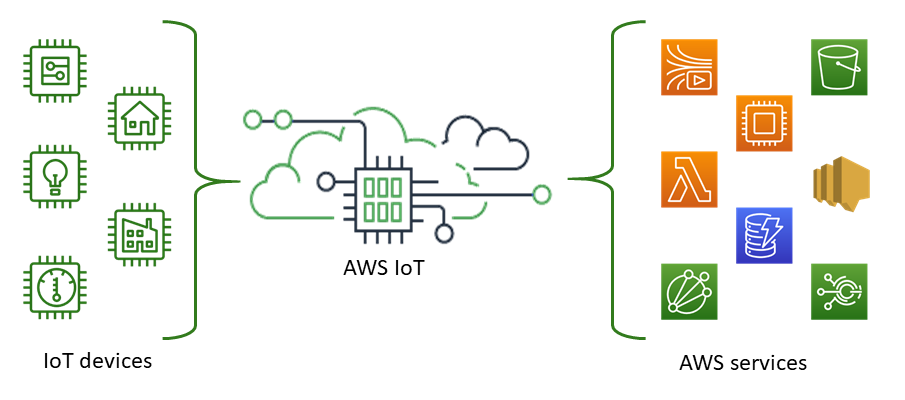
\includegraphics[scale=0.5]{./Figures/aws_iot.png}
	\caption{Diagrama de conexión entre dispositivos IoT y AWS\protect\footnotemark.}
	\label{fig:aws_iot}
\end{figure}
\footnotetext{Imagen tomada de: \url{https://docs.aws.amazon.com/iot/latest/developerguide/what-is-aws-iot.html}}

IoT Core permite seleccionar las tecnologías más adecuadas y actualizadas para interconectar dispositivos IoT. Los protocolos de comunicación soportados son: MQTT, MQTT sobre WSS, HTTPS y LoRaWAN.

El \textit{broker} de IoT Core admite dispositivos y clientes que utilizan MQTT y MQTT sobre WSS para publicar y suscribirse a algún tópico. También es compatible con dispositivos y clientes que utilizan HTTPS para publicar mensajes.

\subsection{Servicio TimeStream}
Timestream es una base de datos de series temporales rápida, escalable y totalmente administrada, que facilita el almacenamiento y el análisis de billones de datos de series temporales al día. Timestream ahorra tiempos y costos con su capacidad de administrar los ciclos de vida de los datos de series temporales, donde mantiene los datos recientes en la memoria y mueve los datos históricos a un nivel de almacenamiento optimizado según las políticas definidas previamente por el usuario. El motor de consultas de Timestream permite acceder y analizar datos recientes e históricos al mismo tiempo. No necesita servidor y su tamaño se acomoda automáticamente para ajustar la capacidad y el rendimiento requeridos \cite{timestream_info}.

Los beneficios más notables que ofrece Amazon Timestream son:
\begin{itemize}
	\item Sin servidor con escalado automático: a medida que cambian las necesidades de la aplicación, Timestream escala automáticamente para ajustar la capacidad.
	\item Administración de los ciclos de vida de los datos: ofrece niveles de almacenamiento, con un almacenamiento de memoria para datos recientes y un almacenamiento magnético para datos históricos. Timestream automatiza el proceso de transferencia entre ambos almacenamientos.
	\item Acceso simplificado a los datos: el motor de consultas de Timestream permite acceder a los datos de forma transparente, sin la necesidad de especificar el nivel de almacenamiento.
	\item Diseñado para series temporales: puede analizar datos de series de tiempo con SQL, con funciones integradas de series de tiempo para suavizar, aproximar e interpolar.
	\item Siempre cifrado: garantiza que los datos de series de tiempo siempre están cifrados. Timestream permite especificar una clave administrada para encriptar datos en el almacenamiento magnético.
	
\end{itemize}

%----------------------------------------------------------------------------------------
\section{Plataforma Grafana}
Es una aplicación web multiplataforma de análisis y visualización interactiva. Proporciona tablas, gráficos y alertas a través de la web cuando se conecta a alguna fuente de datos compatible. Los usuarios pueden crear \textit{dashboards} de monitoreo de datos complejos con ayuda de generadores de consultas interactivos \cite{grafana_info}.

Como herramienta de visualización, Grafana es muy popular gracias a las siguientes características:
\begin{itemize}
	\item Se conecta a muchas fuentes de datos populares como Graphite, Prometheus, Influxdb, ElasticSearch, MySQL, PostgreSQL, entre otros.
	\item Es de código abierto y distribuida bajo la licencia AGPL-3.0, que permite desarrollar complementos desde cero para integrar con otras fuentes de datos.
	\item Ayuda a estudiar, analizar y monitorear datos durante un periodo de tiempo configurable por el usuario.
	\item Puede ser implementado localmente por organizaciones que quieran mantener sus datos confidenciales sin acceso a internet.
	\item Se pueden configurar alertas que se envían por otros medios de comunicación bajo ciertas condiciones preestablecidas.
\end{itemize}




 
\chapter{Diseño e implementación} % Main chapter title

\label{Chapter3} % Change X to a consecutive number; for referencing this chapter elsewhere, use \ref{ChapterX}

\definecolor{mygreen}{rgb}{0,0.6,0}
\definecolor{mygray}{rgb}{0.5,0.5,0.5}
\definecolor{mymauve}{rgb}{0.58,0,0.82}

%%%%%%%%%%%%%%%%%%%%%%%%%%%%%%%%%%%%%%%%%%%%%%%%%%%%%%%%%%%%%%%%%%%%%%%%%%%%%
% parámetros para configurar el formato del código en los entornos lstlisting
%%%%%%%%%%%%%%%%%%%%%%%%%%%%%%%%%%%%%%%%%%%%%%%%%%%%%%%%%%%%%%%%%%%%%%%%%%%%%
\lstset{ %
  backgroundcolor=\color{white},   % choose the background color; you must add \usepackage{color} or \usepackage{xcolor}
  basicstyle=\footnotesize,        % the size of the fonts that are used for the code
  breakatwhitespace=false,         % sets if automatic breaks should only happen at whitespace
  breaklines=true,                 % sets automatic line breaking
  captionpos=b,                    % sets the caption-position to bottom
  commentstyle=\color{mygreen},    % comment style
  deletekeywords={...},            % if you want to delete keywords from the given language
  %escapeinside={\%*}{*)},          % if you want to add LaTeX within your code
  %extendedchars=true,              % lets you use non-ASCII characters; for 8-bits encodings only, does not work with UTF-8
  %frame=single,	                % adds a frame around the code
  keepspaces=true,                 % keeps spaces in text, useful for keeping indentation of code (possibly needs columns=flexible)
  keywordstyle=\color{blue},       % keyword style
  language=[ANSI]C,                % the language of the code
  %otherkeywords={*,...},           % if you want to add more keywords to the set
  numbers=left,                    % where to put the line-numbers; possible values are (none, left, right)
  numbersep=5pt,                   % how far the line-numbers are from the code
  numberstyle=\tiny\color{mygray}, % the style that is used for the line-numbers
  rulecolor=\color{black},         % if not set, the frame-color may be changed on line-breaks within not-black text (e.g. comments (green here))
  showspaces=false,                % show spaces everywhere adding particular underscores; it overrides 'showstringspaces'
  showstringspaces=false,          % underline spaces within strings only
  showtabs=false,                  % show tabs within strings adding particular underscores
  stepnumber=1,                    % the step between two line-numbers. If it's 1, each line will be numbered
  stringstyle=\color{mymauve},     % string literal style
  tabsize=2,	                   % sets default tabsize to 2 spaces
  title=\lstname,                  % show the filename of files included with \lstinputlisting; also try caption instead of title
  morecomment=[s]{/*}{*/}
}

%----------------------------------------------------------------------------------------
\section{Detección facial con TensorFlow y TensorFlow Lite}
\label{section3_1}
Como se explicó en el capitulo \ref{Chapter1}, el objetivo principal de este trabajo es detectar rostros humanos con ayuda de algoritmos de AI. Para esto se deben obtener imagenes digitales con ayuda de una camara, procesarlas y utilizarlas como entrada de una red de modelos de DL capaces de realizar la tarea de deteccion facial. Esta red de modelos de DL fue descrita en el capitulo \ref{Chapter2} y se denomina MTCNN.

Para implementar MTCNN adecuadamente no basta con alimentar P-Net con las imagenes obtenidas por la camara, R-Net con las ventanas candidatas de P-Net y O-Net con las ventanas candidatas de R-Net. Los datos de entrada de cada uno de los modelos de MTCNN deben ser procesados para conseguir el mejor resultado posible, como se muestra en el diagrama de la figura \ref{fig:mtcnn_npipe}.

\begin{figure}[h]
	\centering
	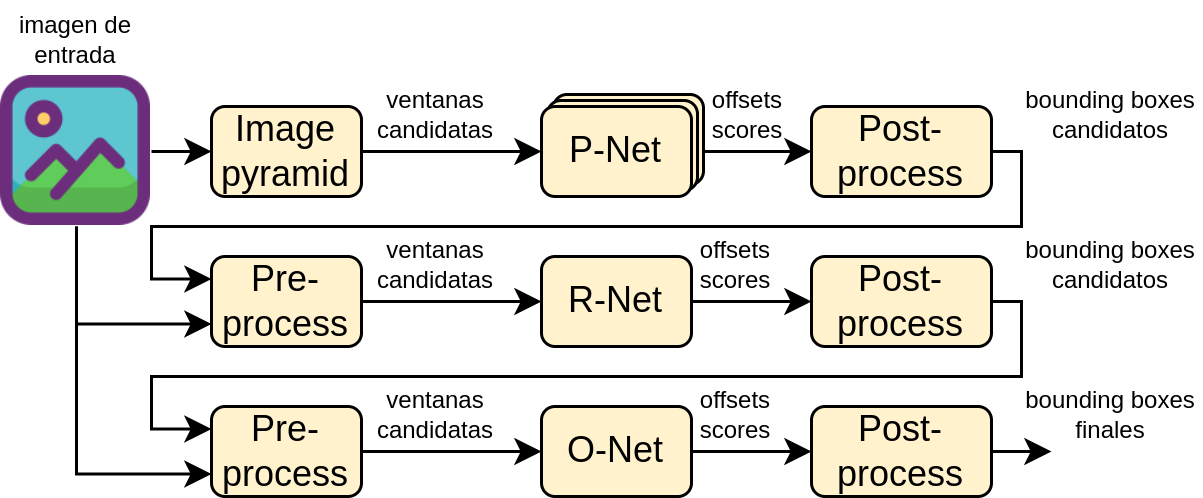
\includegraphics[scale=0.3]{./Figures/mtcnn_npipe.png}
	\caption{\textit{Pipeline} detallado de MTCNN.}
	\label{fig:mtcnn_npipe}
\end{figure}

El diagrama de la figura \ref{fig:mtcnn_npipe} muestra el \textit{pipeline} detallado de la red MTCNN, donde se pueden observar varios bloques de procesamiento, estos son:

\begin{itemize}
	\item \textit{Image pyramid}: genera a partir de la imagen de entrada otras imágenes de escalas inferiores, lo que permite detectar objetos de distintos tamaños. Cada nivel de escala se obtiene mediante la reducción de la escala anterior, por lo que las imágenes en niveles superiores tienen una escala mas baja que las imagenes en niveles inferiores. Después de generadas las imágenes escaladas requeridas de la imagen de entrada estas sirven para alimentar P-Net y así detectar rostros de distintos tamaños.

	\item \textit{Post-process}: en este bloque se procesan los datos de salida generados por P-Net, R-Net y O-Net. El primer subbloque realiza la operación de NMS para reducir la cantidad de ventanas candidatas que tienen solapmiento entre ellas. El segundo subbloque aplica un proceso de calibración que utiliza los \textit{offsets} generados por los modelos para determinar de manera mas precisa las coordenadas de las ventanas candidatas. Finalmente el último subbloque corrige las coordenadas de las ventanas candidatas para que posean dimensiones cuadradas y estén dentro de los límites de la imagen original.
	\begin{figure}[h]
		\centering
		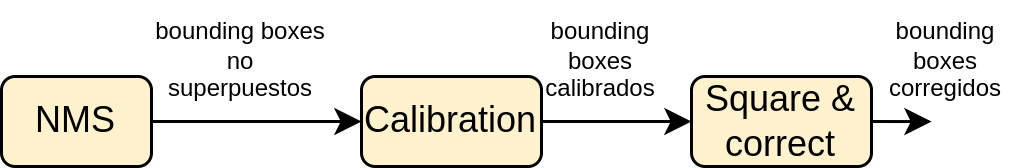
\includegraphics[scale=0.35]{./Figures/mtcnn_postprocess.png}
		\caption{Bloque de postprocesamiento.}
		\label{fig:mtcnn_postprocess}
	\end{figure}
	
	\item \textit{Pre-process}: tiene la función de procesar los datos de entrada para las redes R-Net y O-Net. El primer subbloque genera recortes de la imagen original en función de las coordenadas obtenidas del bloque \textit{post-process}. En el segundo subbloque las imágenes recortadas de entrada son redimensionadas con dimensiones de 24x24 px y 48x48 px, para alimentar R-Net y O-Net respectivamente.`
	\begin{figure}[h]
		\centering
		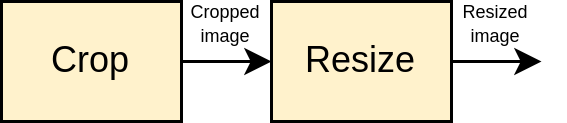
\includegraphics[scale=0.35]{./Figures/mtcnn_preprocess.png}
		\caption{Bloque de preprocesamiento.}
		\label{fig:mtcnn_preprocess}
	\end{figure}

\end{itemize}

P-Net, R-Net y O-Net fueron creados con ayuda de la biblioteca para redes neuronales Keras, que es parte del \textit{core} de TensorFlow, de acuerdo con lo expuesto en \cite{mtcnn_info}. Para P-Net se crearon tantos modelos como escalas utilizadas, en este caso 3, suficientes para detectar rostros a corta distancia. Con las arquitecturas definidas de los modelos el siguiente paso natural en el desarrollo deberia haber sido su entrenamiento con uno o varios \textit{datasets}, pero al ser MTCNN tan popular en el ambito de deteccion facial se pudieron encontrar archivos de tipo HDF (\textit{Hierarchical Data Format}, Formato de Datos Jerárquicos) que contenian los \textit{weights} resultantes de un proceso de entrenamiento anterior. En el siguiente fragmento de codigo se puede observar el código utilizado para crear O-Net.

Para que los modelos obtenidos pudieran ser ejecutados en el hardware objetivo de este trabajo tuvieron que ser convertidos a un formato más liviano y eficiente llamado TensorFlow Lite. El conversor de TensorFlow Lite toma un modelo de TensorFlow y genera un moelo de TensorFlow Lite cuya extensión de archivo es .tflite. La conversión puede seguir 2 caminos según como sean evaluados los modelos de TensorFlow, en la figura \ref{fig:tf2tflite_workflow} se observa el flujo de trabajo del conversor.

\begin{figure}[h]
	\centering
	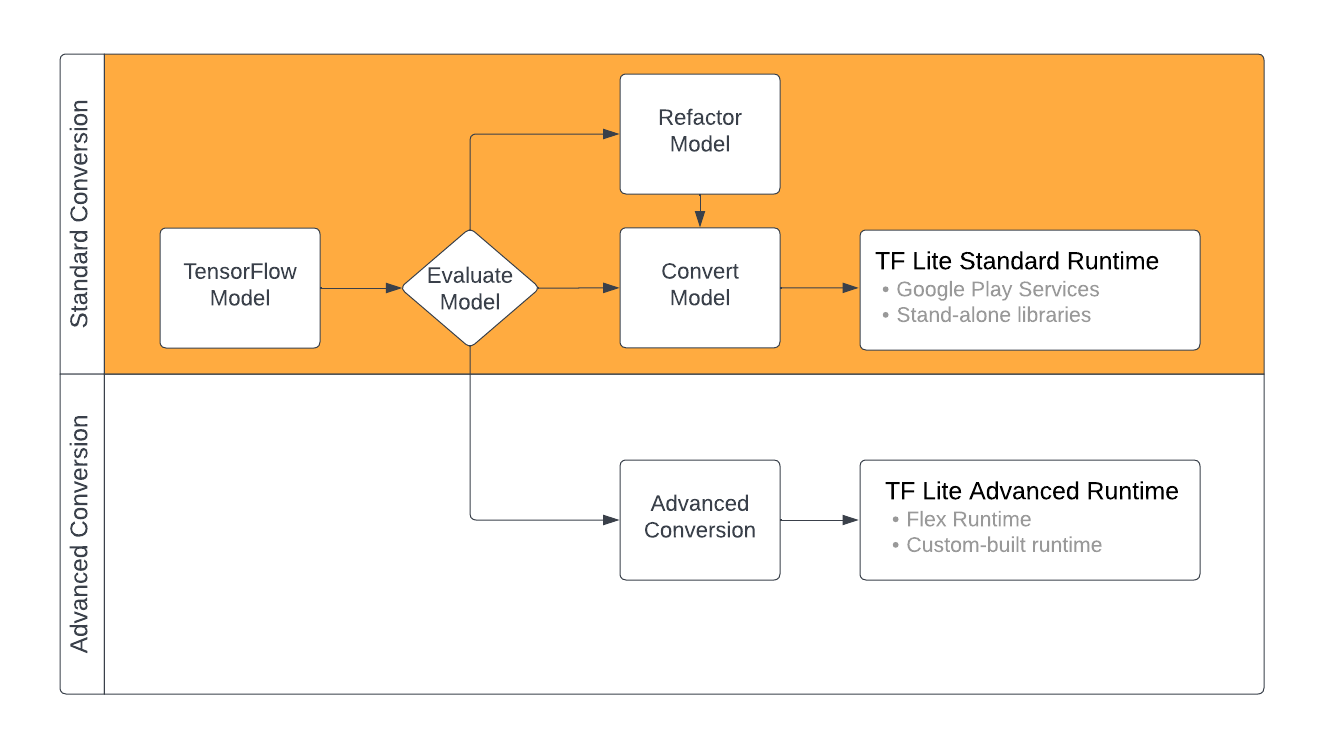
\includegraphics[scale=0.6]{./Figures/tf_convert_workflow_diag.png}
	\caption{Diagrama de flujo de trabajo para la conversion\protect\footnotemark.}
	\label{fig:tf2tflite_workflow}
\end{figure}
\footnotetext{Imagen tomada de: \url{https://www.tensorflow.org/lite/models/convert/}}

Gracias a que todos los operadores utilizados en los modelos de TensorFlow eran compatibles con los operadores de TensorFlow Lite se realizó una conversión estandar, lo que posteriormente facilitó su implementación en el hardware destino.

Durante el proceso de conversión se se aplicaron optimizaciones que responden a una necesidad de reducir aún más el tamaño y la latencia de los modelos. Se realizó una optmización por cuantización, que se refiere a la reducción de la precisión de los numeros usados para representar los parametros de los modelos, los cuales por defecto son flotantes de 32 bits. Las opciones de cuantización para los modelos se tomaron del diagrama de la figura \ref{fig:tf_quantization_tree}.

\begin{figure}[h]
	\centering
	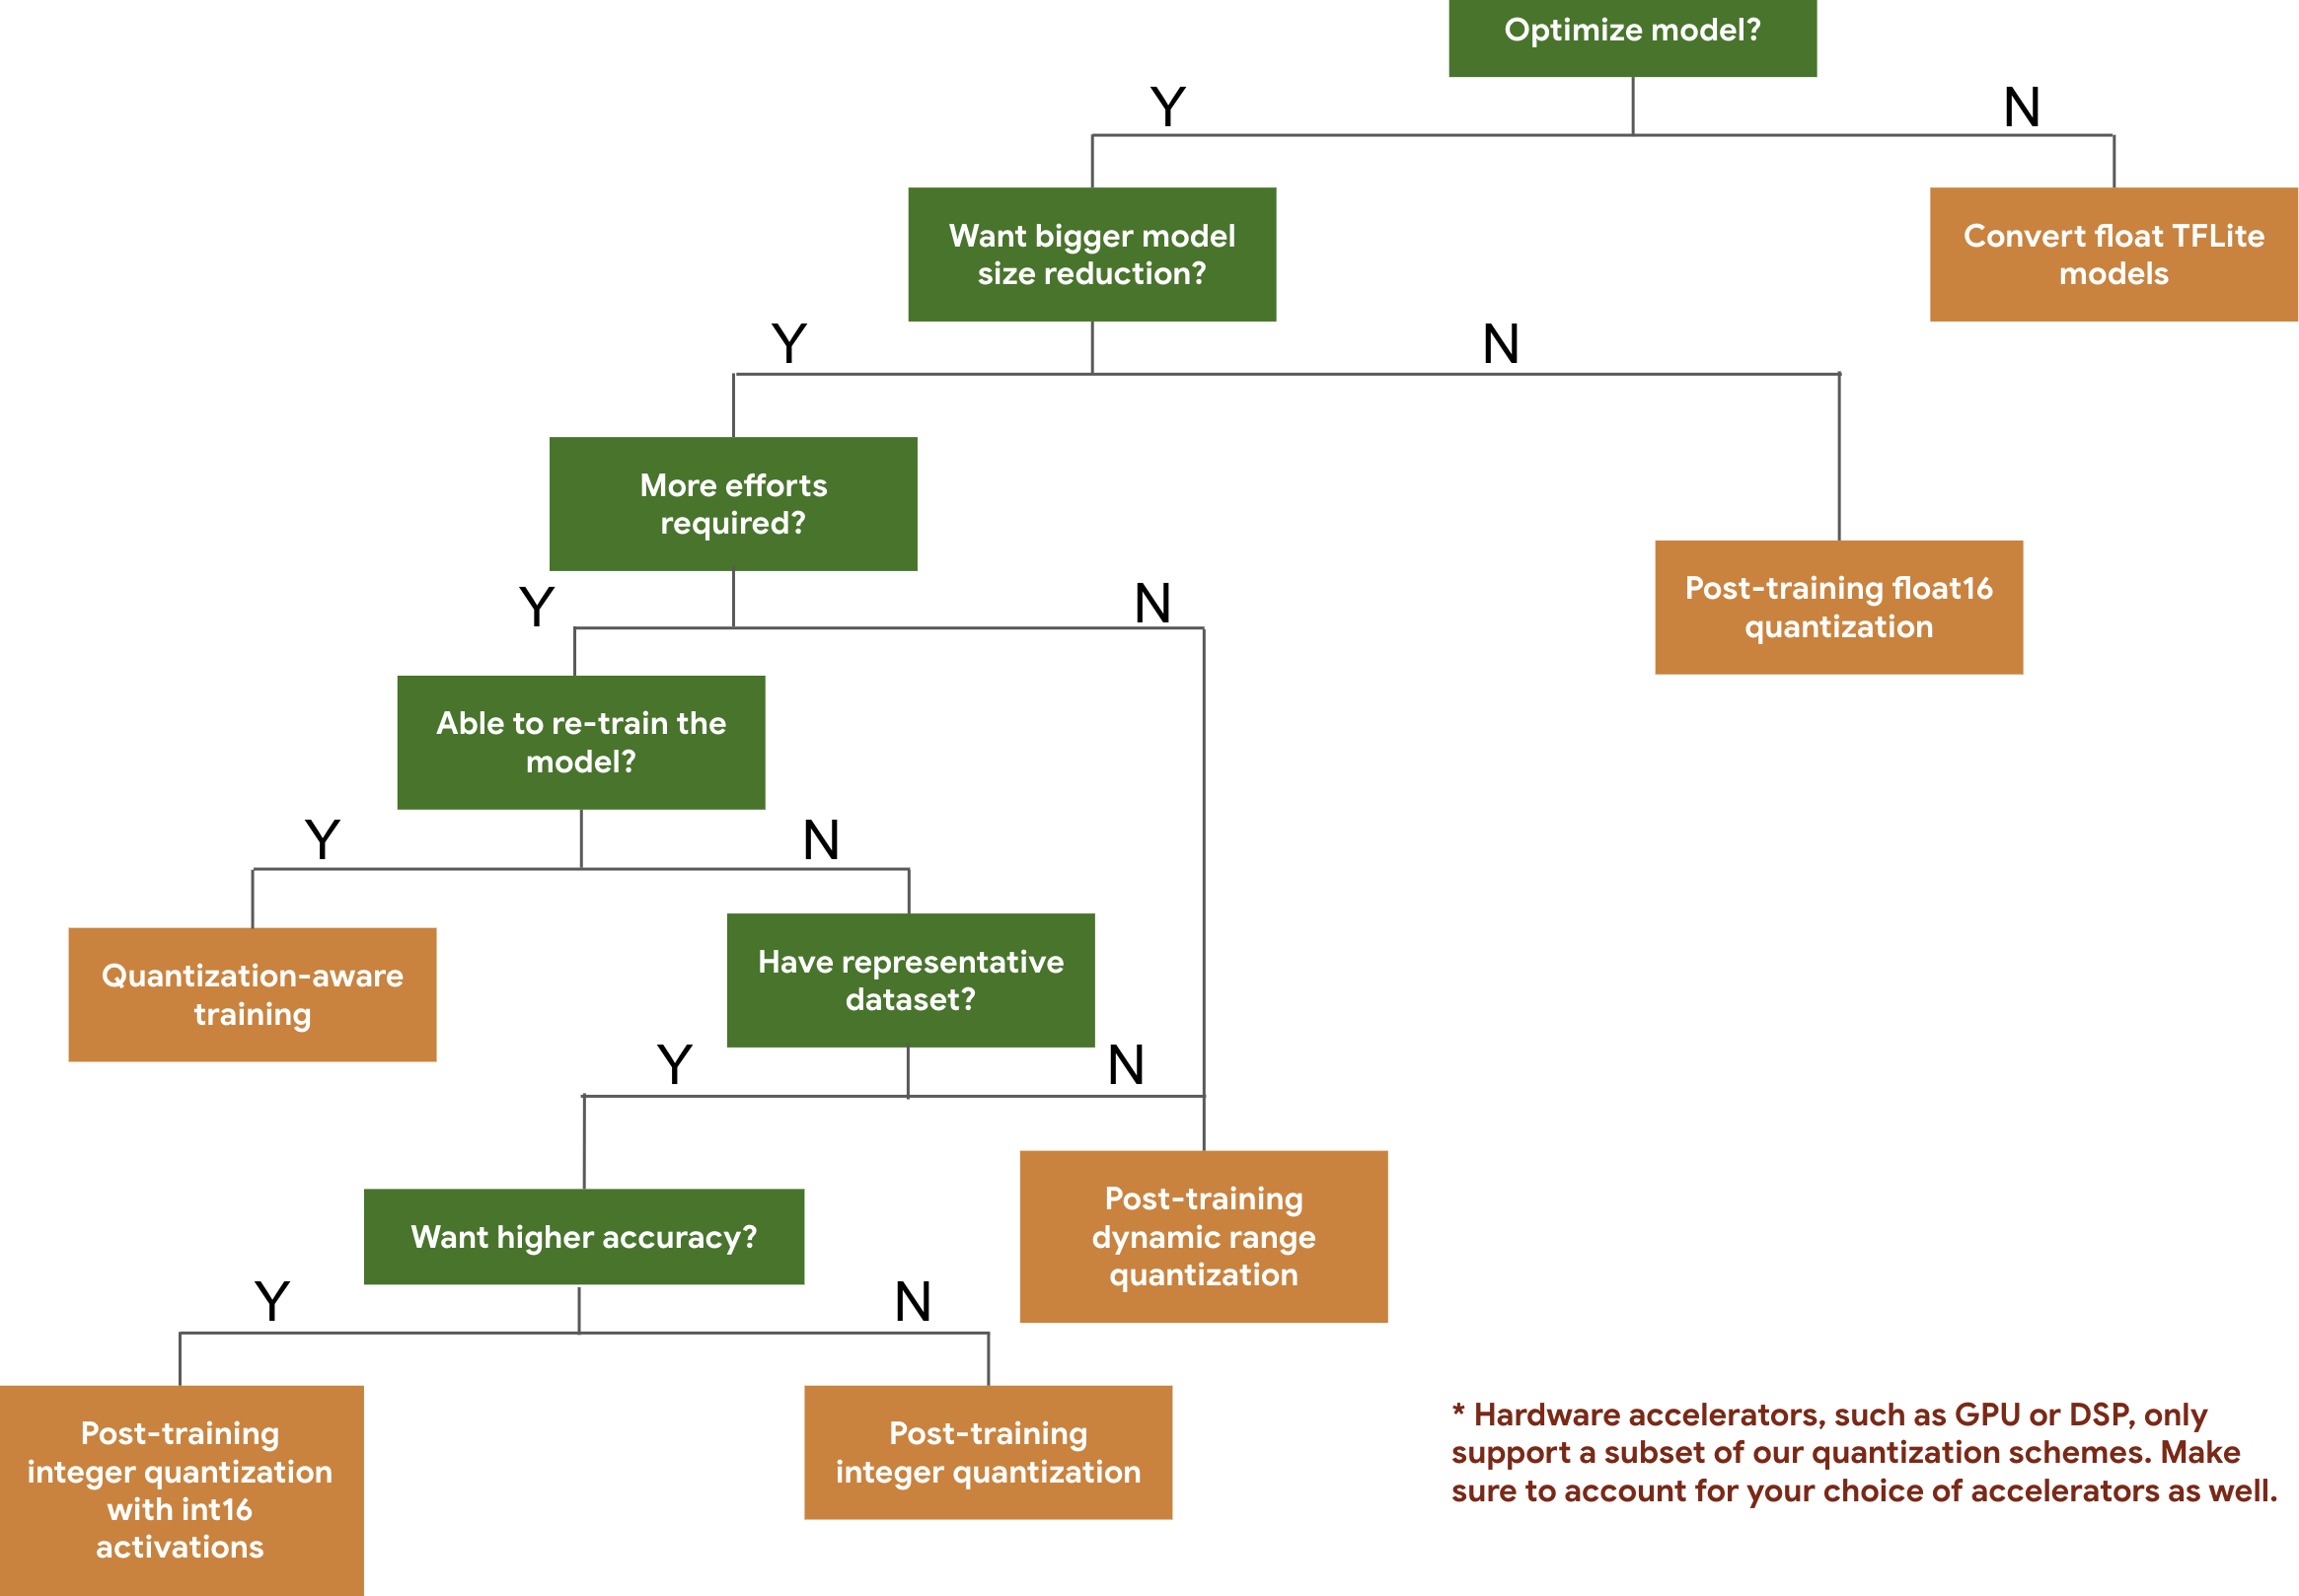
\includegraphics[scale=0.3]{./Figures/tf_quantization_decision_tree.png}
	\caption{Diagrama de árbol de decisiones para el proceso de cuantización\protect\footnotemark.}
	\label{fig:tf_quantization_tree}
\end{figure}
\footnotetext{Imagen tomada de: \url{https://www.tensorflow.org/lite/performance/model_optimization}}

La cuantizacion utilizada para los modelos fue \textit{full integer quantization}, que reduce los picos de memoria utilzados y asegura la compatibilidad con dispositivos de hardware que no pueden utilizar punto flotante. Para este tipo de cuantización se necesito crear un \textit{dataset} representativo, compuesto por un pequeno subconjunto (entre 100 a 500 muestras) del \textit{dataset} de entrenamiento. En ... se expone el codigo utilizado para la conversión de los modelos al formato TensorFlow Lite con cuantización a 8 bits.

La tabla \ref{tab:models_comp} muestra las diferencias entre los tamaños y latencias obtenidas para el modelo O-Net de TensorFlow, TensorFlow Lite sin quantización y TensorFlow Lite con cuantizacion a 8 bits.

\begin{table}[h]
	\centering
	\caption[Modelos comparativa]{Tabla comparativa de O-Net}
	\begin{tabular}{lcc}   
		\toprule
		\textbf{TensorFlow} & \textbf{TensorFlow Lite} & \textbf{TensorFlow Lite int8} \\
		\midrule
		Tamaño (bytes) & 2 V a 15 V & x \\
		Latencia (ms) & 2 V a 15 V & x \\
		\bottomrule
		\hline
	\end{tabular}
	\label{tab:models_comp}
\end{table}

Todo el código para la obtención de los modelos hasta aquí expuesto, las funciones del \textit{pipeline}, las pruebas realizadas a los modelos y el despliegue de estos en el SoC ESP32-S3, se encuentra disponible en el repositorio de acceso público \cite{mtcnn_repo}.

%----------------------------------------------------------------------------------------
\section{Desarrollo del firmware}
El primer paso para el desarrollo del firmware del dispositivo fue la elección de un conjunto de herramientas de software o SDK (\textit{Software Development Kit}, Kit de Desarrollo de software) por sus siglas en inglés. Estas herramientas permitieron implementar código para utilizar de manera eficiente todos los periféricos disponibles en el ESP32-S3. Para este proyecto el SDK utilizado fue ESP-IDF \cite{idf_repo}, las razones de su elección fueron:
\begin{itemize}
	\item Experiencia:
	\item Compatibilidad:
	\item Herramientas:
	\item Soporte:
	\item Documentación:
\end{itemize}

Con el conjunto de herramientas definido, otro aspecto de importancia fue la elección de un entorno de desarrollo para optimizar la escritura y depuración de código. El IDE (\textit{Integrated Development Environment}, Entorno de Desarrollo Integrado) escogido fue Eclipse IDE C/C++, los aspectos más importantes para su elección fueron:
\begin{itemize}
	\item Experiencia:
	\item Herramientas:
	\item Complementos: 
\end{itemize}

Otra herramienta importante para el proceso de desarrollo del firmware fue la utlización de sofware para control de versiones, que permite realizar un seguimiento de los cambios realizados en el código a lo largo del tiempo. Git fue elegido como software de control de versiones, mientras que GitHub como plataforma para alojar el repositorio de Git. Las razones para la elección de ambos son:
\begin{itemize}
	\item Experiencia:
	\item Reutilización de código:
	\item Soporte:
	\item Documentación:
\end{itemize}

Con todas las herramientas de software correctamente seleccionadas, el siguiente paso fue el diseño de la arquitectura del firmware. El firmware desarrollado siguió una arquitectura en capas, donde las capas de niveles más bajos tienen una mayor interacción con el hardware, mientras que las de niveles más altos con la aplicación del usuario. En la figura \ref{fig:fw_layers} se presenta el diagrama en capas del firmware.

\begin{figure}[h]
	\centering
	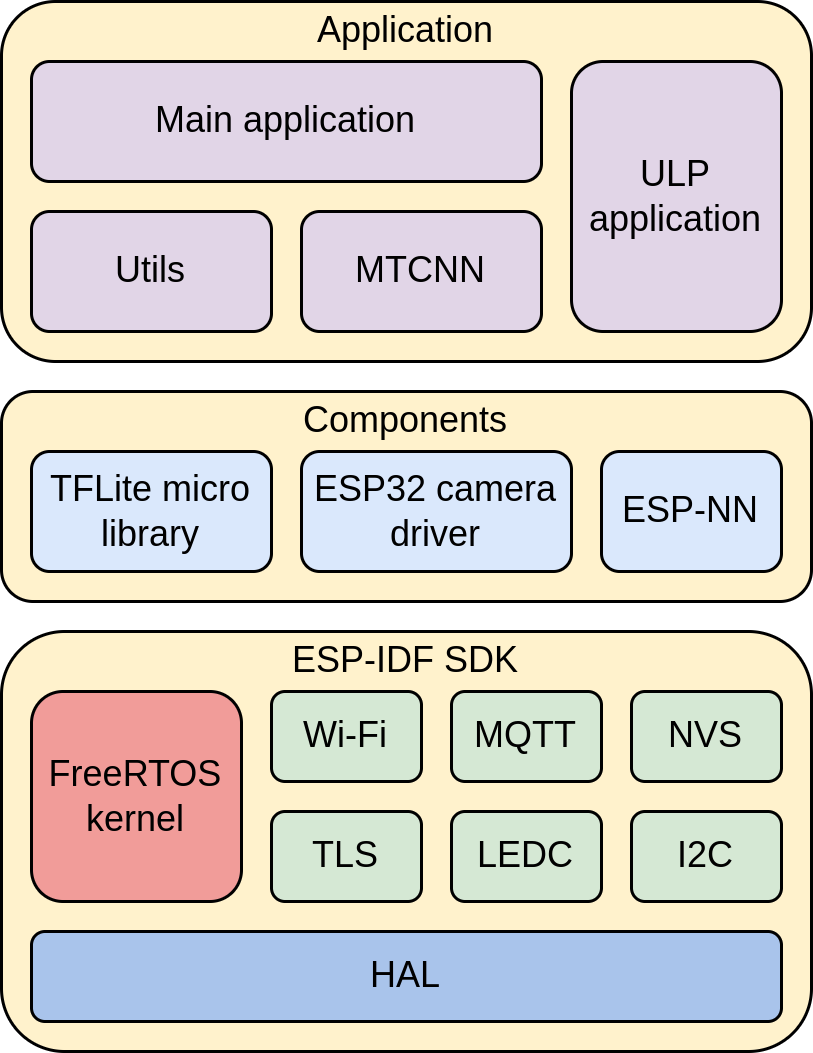
\includegraphics[scale=0.25]{./Figures/fw_layers.png}
	\caption{Diagrama de capas del firmware.}
	\label{fig:fw_layers}
\end{figure}

Las capas expuestas en el diagrama de la figura \ref{fig:fw_layers} son:
\begin{itemize}
	\item ESP-IDF SDK:
	\item \textit{Components}:
	\begin{itemize}
		\item TFLite micro library:
		\item ESP32 camera driver:
		\item ESP-NN:
	\end{itemize}
	\item \textit{Application}:
	\begin{itemize}
		\item \textit{Main application}:
		\item \textit{Main application}:
		\item MTCNN:
		\item \textit{Utils}:
	\end{itemize}
\end{itemize}

El firmware desarrollado cumple con las siguientes tareas: detección facial con TensorFlow Lite para microcontroladores, comunicación con los servicios en la nube y gestión del consumo energético.

\subsection{Deteccion facial con TensorFlow Lite para microontroladores}
En la sección \ref{section3_1} se obtuvieron los modelos para MTCNN en los formatos TensorFlow, TensorFlow Lite y TensorFlow Lite para microcontroladores. El objetivo de esta tarea es obtener imágenes con la cámara del sistema para procesarlas con los modelos de MTCNN y determinar la cantidad  de rostros humanos existentes en cada imagen. El diagrama de flujo de la figura \ref{fig:fw_detect_flow} detalla el proceso de esta tarea.

\begin{figure}[h]
	\centering
	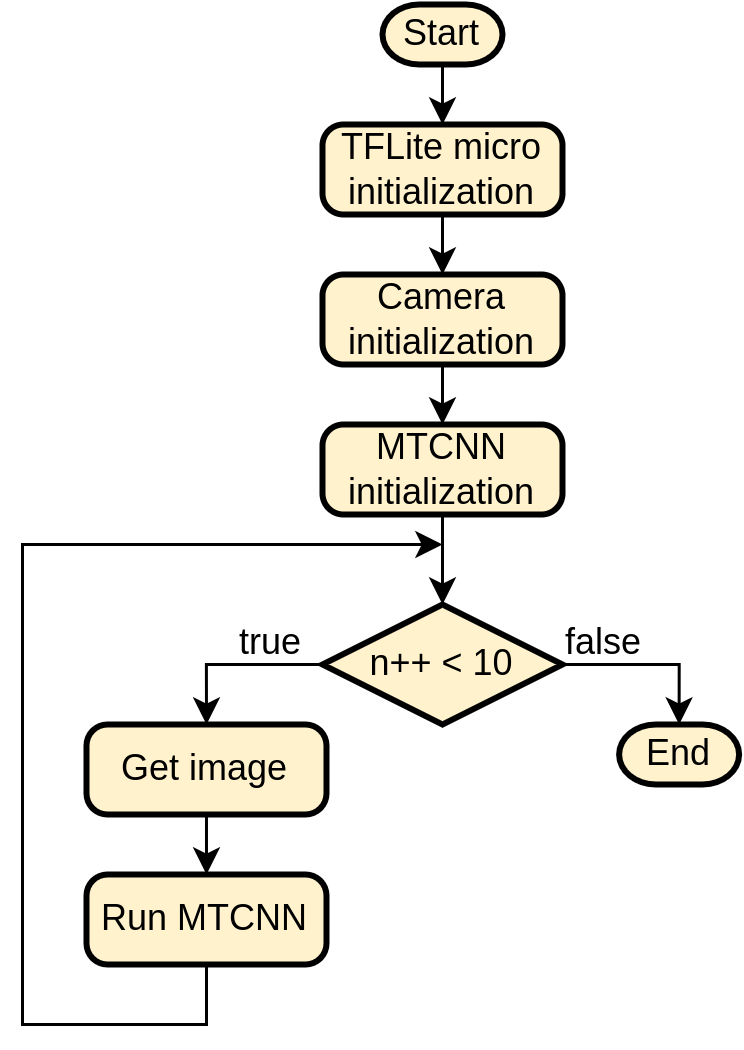
\includegraphics[scale=0.22]{./Figures/fw_detection_flow.png}
	\caption{Diagrama de flujo de la tarea de detección facial.}
	\label{fig:fw_detect_flow}
\end{figure}

El proceso de inicialización de TFLite micro requiere de varios pasos que deben ser seguidos en orden para poder ejecutar los modelos de MTCNN correctamente. En el fragmento de codigo ... se presenta la inicialización para O-Net con TFLite micro.

\begin{lstlisting}[label=cod:tflm_init,caption=Código para inicializar O-Net con TFLite micro.]
/* Map the model into a usable data structure */
const tflite::Model *onet_model = tflite::GetModel(onet_model_data);

/* Reserve memory for the tensors */
uint8_t *tensor_arena = (uint8_t *)heap_caps_malloc(TENSOR_ARENA_SIZE, MALLOC_CAP_SPIRAM | MALLOC_CAP_8BIT);

/* Pull in only the operation implementations needed */
static tflite::MicroMutableOpResolver<10> micro_op_resolver;
micro_op_resolver.AddAveragePool2D();
micro_op_resolver.AddConv2D();
micro_op_resolver.AddPrelu();
micro_op_resolver.AddMaxPool2D();
micro_op_resolver.AddTranspose();
micro_op_resolver.AddFullyConnected();
micro_op_resolver.AddDequantize();
micro_op_resolver.AddDepthwiseConv2D();
micro_op_resolver.AddReshape();
micro_op_resolver.AddSoftmax();

/* Build an interpreter to run the model with */
static tflite::MicroInterpreter static_onet_interpreter(onet_model, micro_op_resolver, tensor_arena, TENSOR_ARENA_SIZE);
onet_interpreter = &static_onet_interpreter;

/* Allocate memory from the tensor_arena for the model's tensors */
onet_interpreter->AllocateTensors();
\end{lstlisting}

Los modelos de P-Net y R-Net se inicializan de la misma forma que O-Net y una cosa a notar es la declaración de los operadores estrictamente necesarios para ejecutar estos modelos en las líneas 9-18. Otra aproximación más sencilla era utilizar \texttt{OpsResolver} para utilizar todos los operadores, pero esto hubiera supuesto una penalización en la cantidad de memoria RAM utilizada. En la figura \ref{fig:fw_tflite_ops} se puede observar una captura de pantalla de una página web generada con la herramienta de visualización de modelos de TensorFlow Lite que se encuentra en el repositorio oficial de TensorFLow Lite para microcontroladores\cite{tflm_repo}, donde se muestran los operadores utilizados por O-Net.

\begin{figure}[h]
	\centering
	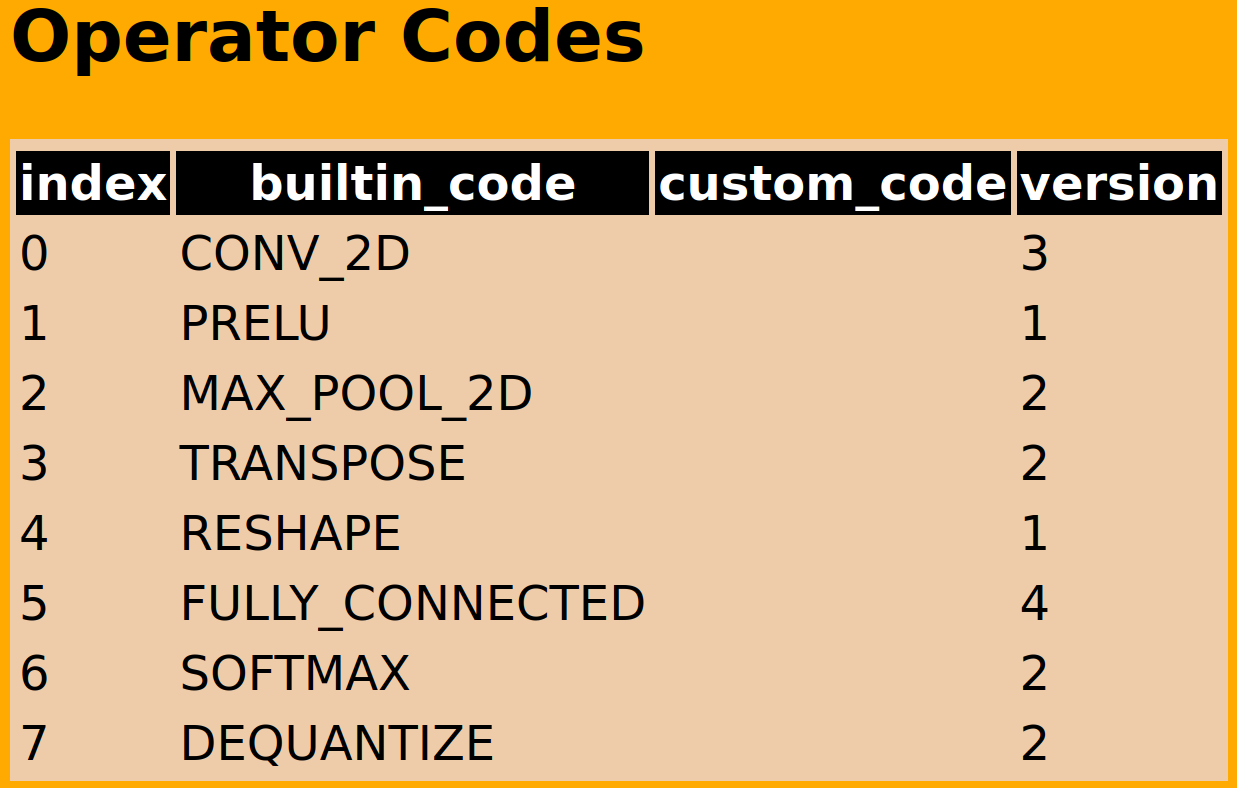
\includegraphics[scale=0.18]{./Figures/fw_tflite_ops.png}
	\caption{Captura de pantalla del detalle del modelo O-Net para TensorFlow Lite.}
	\label{fig:fw_tflite_ops}
\end{figure}

Otro aspecto a destacar es la utilización de la memoria PSRAM (\textit{Pseudo static} RAM, RAM Pseudoestática) para almacenar los tensores utilizados durante la ejecucióin de los modelos de MTCNN. En la línea 5 del fragmento de código ... se puede observar como se reserva memoria en la PSRAM de un tamaño determinado de manera experimental y denominado \texttt{TENSOR\_ARENA\_SIZE}.

Los métodos de MTCNN para inicializarlo y ejecutar sus modelos se encuentran en los archivos \texttt{main/mtcnn.h} y \texttt{mtcnn.cc} del repositorio \cite{mtcnn_repo}. En el fragmento de código ... se pueden observar las estructuras de datos utilizadas por los métodos de MTCNN.

\begin{lstlisting}[label=cod:mtcnn_struct,caption=Estructura de datos de MTCNN.]
typedef struct {
  tflite::MicroInterpreter *interpreter;
  candidate_windows_t candidate_windows;
  bboxes_t bboxes;
} model_data_t;

typedef struct {
  model_data_t pnet[3];
  model_data_t rnet;
  model_data_t onet;
} mtcnn_t;
\end{lstlisting}

Como el tipo de dato \texttt{mtcnn\_t} contiene todos los datos de entrada y salida de los modelos de MTCNN, fue utilizado como parámetro de todas las funciones encargadas de ejecutar los modelos. La función que ejecuta O-Net es \texttt{mtcnn\_run\_onet} y en el fragmento de código ... se puede observar su implementación.

\begin{lstlisting}[label=cod:mtcnn_struct,caption=Función mtcnn\_run\_onet.]
void mtcnn\_run_\onet(mtcnn_t *mtcnn, uint8_t *img, uint16_t img_w, uint16_t img_h) {
  /* Pre-process R-Net ouputs */
  
  /* Feed the model and run it */
  TfLiteTensor *input = mtcnn->interpreter->input(0);
    
  for(int i = 0; i < ONET_SIZE * ONET_SIZE * 3; i++) {
    input->data.int8[i] = ((uint8_t *) onet_image)[i] ^ 0x80;
  }
  
  mtcnn->interpreter->Invoke();
  
  /* Store the scores and offsets output */
  TfLiteTensor *scores = interpreter->output(0);
  
  for(uint8_t j = 0; j < 2; j++) {
    probs_buf[j + (i * 2)] = probs->data.f[j];
  }

  TfLiteTensor *offsets = interpreter->output(1);

  for(uint8_t j = 0; j < 4; j++) {
    offsets_buf[j + (i * 2)] = offsets->data.f[j];
  }
  
  /* Add the candidate windows to the candidate windows array */
  add_candidate_windows();
  
  /* Post-process O-Net ouputs */
}
\end{lstlisting}

\subsection{Comunicación con los servicios en la nube}
Esta tarea fue diseñada para establecer conectividad con los servicios en la nube, más precisamente con el servicio IoT Core de AWS, para transmitir y recibir datos mediante el protocolo MQTT (MQ \textit{Telemetry Transport}, Transporte de Telemetría MQ). El diagrama de flujo de la figura \ref{fig:fw_comm_flow} muestra el proceso que sigue esta tarea.

\begin{figure}[h]
	\centering
	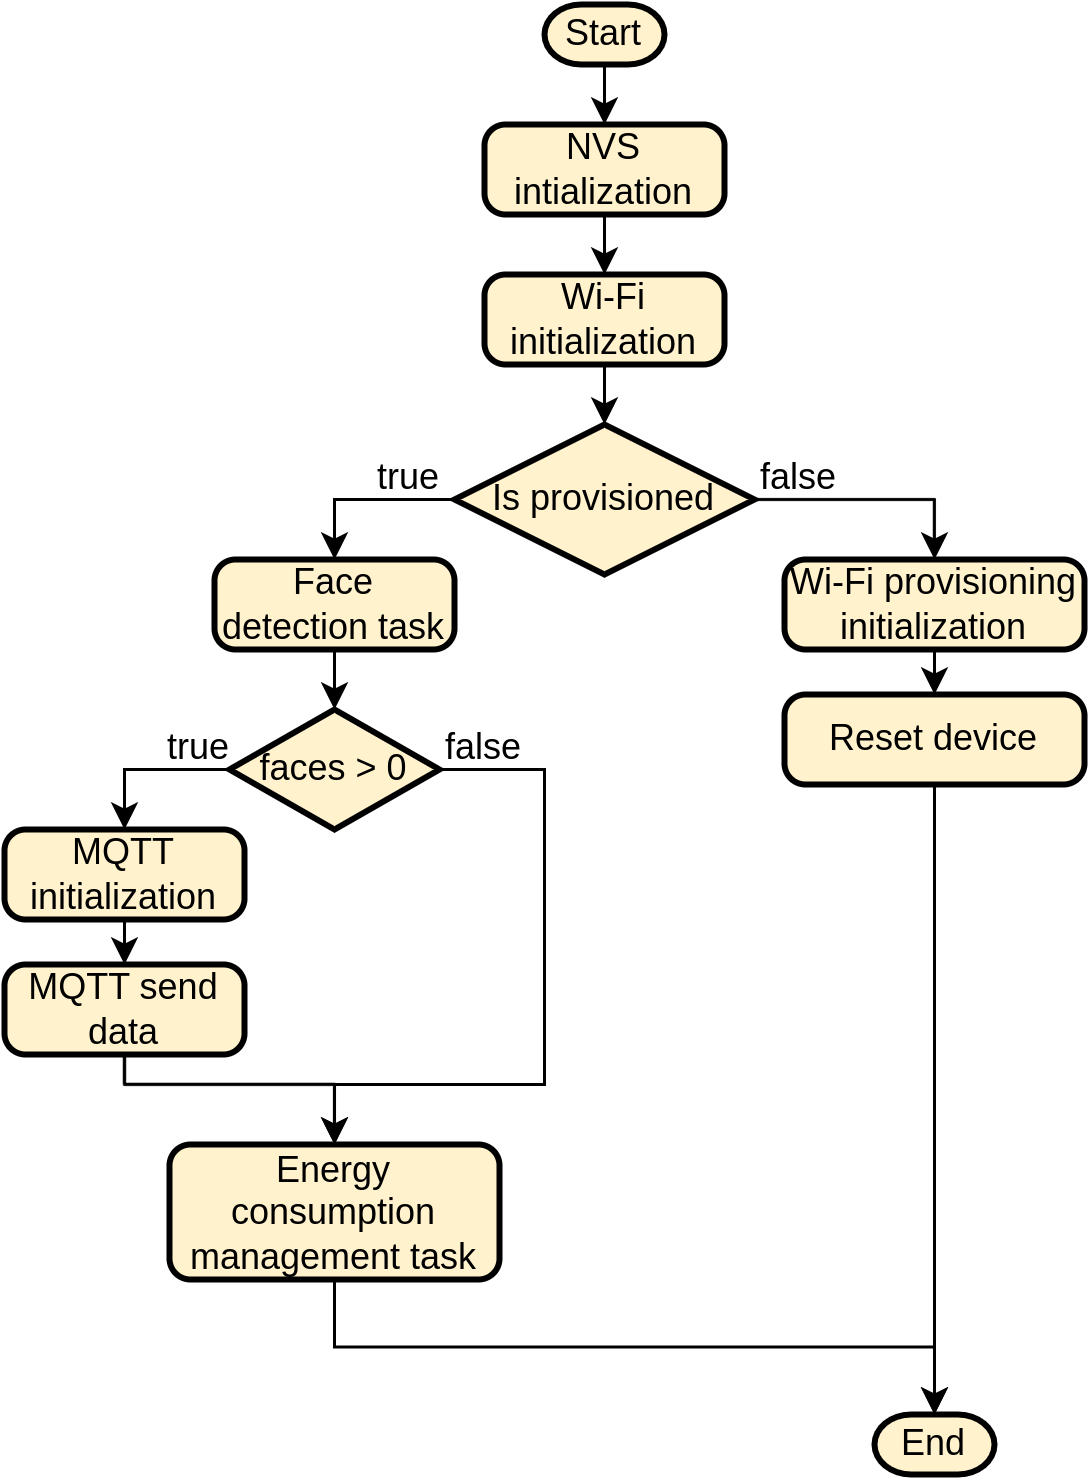
\includegraphics[scale=0.22]{./Figures/fw_comm_flow.png}
	\caption{Diagrama de flujo de la tarea de comunicación con los servicios en la nube.}
	\label{fig:fw_comm_flow}
\end{figure}

El digrama de la figura \ref{fig:fw_comm_flow} empieza con la inicialización de la memoria NVS y el perférico Wi-Fi en modo punto de acceso y estación, para después establecer si el dispositivo debe ejecutar el proceso de provisionamiento de credenciales Wi-Fi o en cambio ejecutar la tarea de detección facial y transmitir los datos generados. El provisionamiento de credenciales Wi-Fi utiliza un protocolo de comunicación llamado protocomm (\textit{protocol communication}) de Espressif \cite{protocomm_doc} y corre sobre Wi-Fi en modo SoftAP (\textit{Software enabled Access Point}, Punto de Acceso habilitado por Software). En el fragmento de código ... se exhiben las línea de código para la inicializacion del provisionamiento Wi-Fi.

\begin{lstlisting}[label=cod:mtcnn_struct,caption=Función mtcnn\_run\_onet.]
/* Initalize Wi-Fi provisioning over SoftAP */
wifi_prov_mgr_config_t prov_config = {
  .scheme = wifi_prov_scheme_softap,
  .scheme_event_handler = WIFI_PROV_EVENT_HANDLER_NONE,
  .app_event_handler = WIFI_PROV_EVENT_HANDLER_NONE
};

ESP_ERROR_CHECK(wifi_prov_mgr_init(prov_config));
\end{lstlisting}

Cuando se ejecuta la tarea de detección facial pueden o no detectarse rostros humanos en la imágenes obtenidas por la cámara, cuando uno más rostros son detectados esta información se transmite por MQTT. AWS IoT Core dispone de un \textit{broker} MQTT que implementa TLS (\textit{Transport Layer Security}, Seguridad de la Capa de Transporte) \cite{tls_doc} para brindar seguridad en el intercambio de mensajes, por tanto, la autenticacíon y cifrado de datos necesita de certificados y llaves para llevarse a cabo. La llave privada y el certificado del dispositivo son generados en la plataforma AWS IoT Core y deben quedar grabadas en la memoria del ESP32-S3 para que puedan ser utilizadas en el código. La forma más simple de utilizar la llave y el certificado es añadirlas al binario de la aplicación durante el proceso de compilación, en la figura \ref{fig:fw_parttab1} se observa un diagrama representativo de la distribución de la memoria del ESP32-S3, donde los valores encima de los bloques son las posiciones de memoria donde se encuentran las particiones y los valores que se encuentran por debajo son la cantidad de memoria utilizada.

\begin{figure}[h]
	\centering
	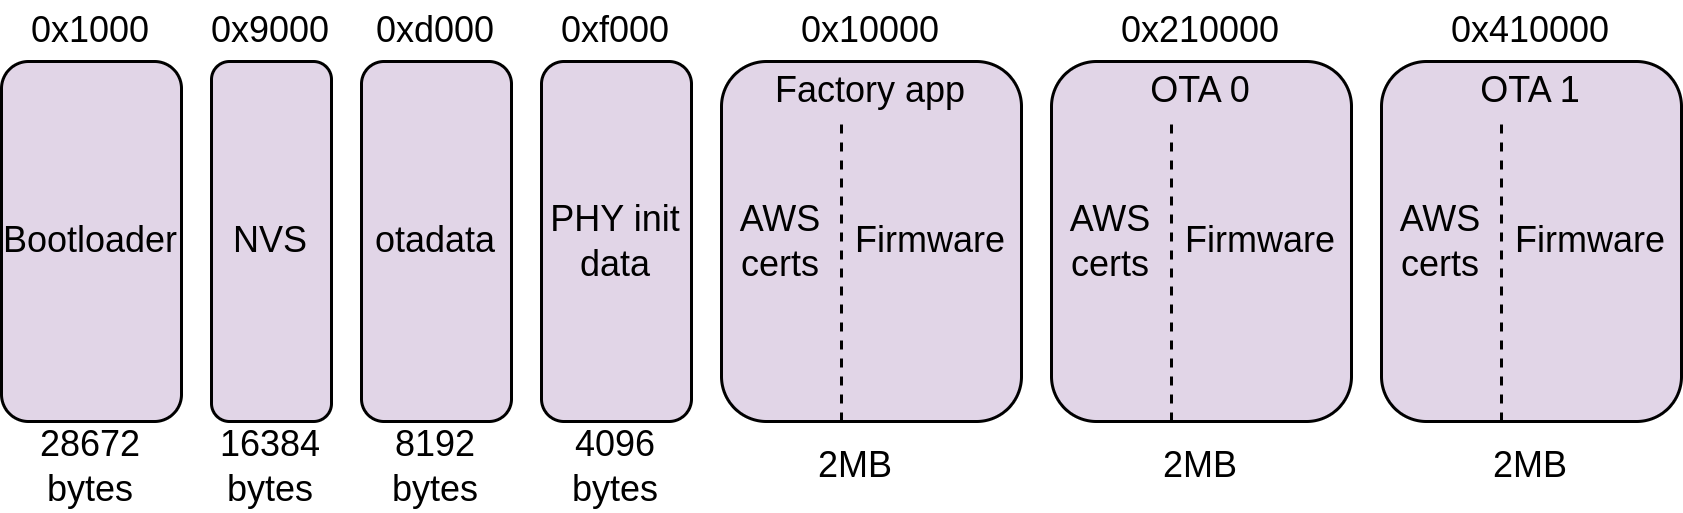
\includegraphics[scale=0.22]{./Figures/fw_parttab1.png}
	\caption{Diagrama representativo de la memoria del ESP32-S3.}
	\label{fig:fw_parttab1}
\end{figure}

En el diagrama de la figura \ref{fig:fw_parttab1} se puede observar un problema no menor con respecto a al proceso de actualizaciones OTA, que las actualizaciones sobreescribirán tanto el \textit{firmware} como el certificado y llave privada del dipositivo. Esto no sería problemático para un solo dispotivo, pero si existieran más dispositivos establecerian conexión con AWS IoT Core con el mismo certificado y llave privada, lo que supondría una grave falla de seguridad de la información. Para corregir esta falla de seguridad se optó por generar llaves y certificados únicos para cada dispositivo, y grabarlos en la memoria NVS en un \textit{namespace} llamado "certs", de esta forma el proceso de actualización OTA solo sobreescribirá el \textit{firmware} más no el certificado ni la llave. En la figura \ref{fig:fw_parttab2} se muestra el diagrama representativo de la memoria del ESP32-S3 utilziado en este trabajo.

\begin{figure}[h]
	\centering
	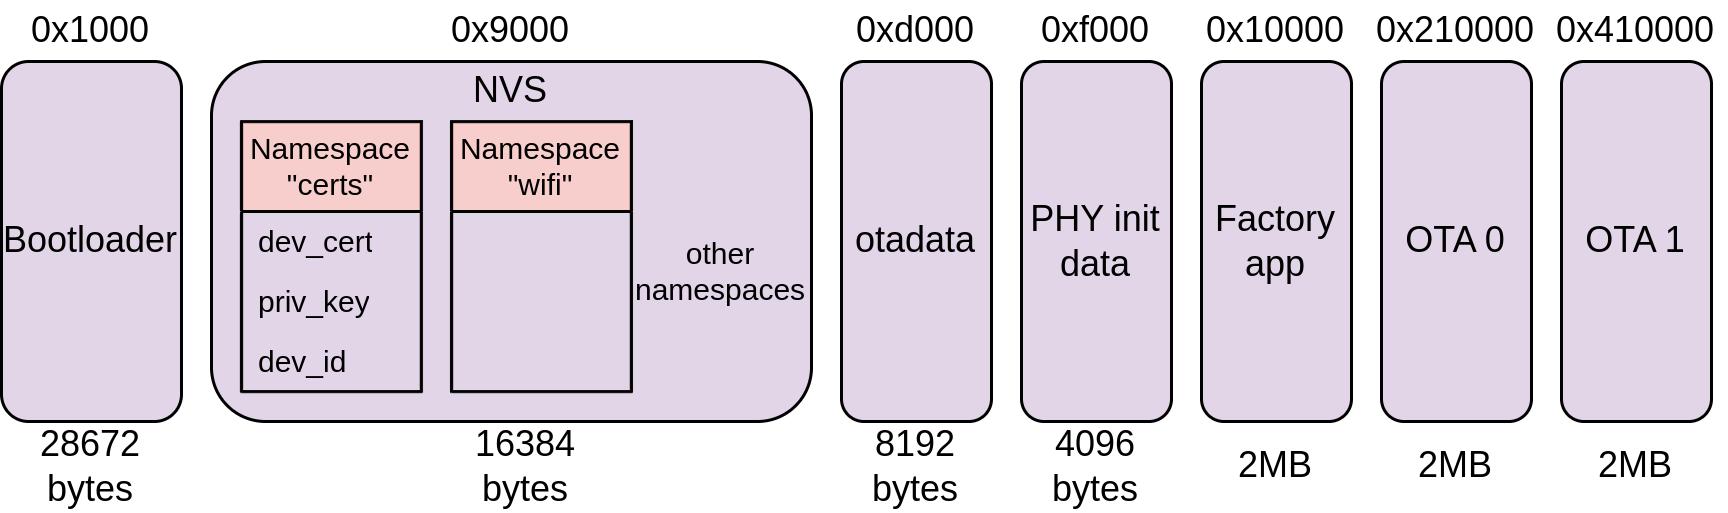
\includegraphics[scale=0.22]{./Figures/fw_parttab2.png}
	\caption{Diagrama representativo de la memoria del ESP32-S3.}
	\label{fig:fw_parttab2}
\end{figure}

La inicialización de MQTT en el código utiliza una estructura de datos donde algunoss campos debens ser asignados al certificado del dispositivo y la llave privada en formato de cadena de caracteres. En los fragmentos de codigo ... se exhibe la función para obtener una cadena de caracteres de la NVS y la inicialización de MQTT en modo cliente.

\begin{lstlisting}[label=cod:mtcnn_struct,caption=Función para cargar una cadena de caracteres de la NVS.]
esp_err_t load_string_from_nvs(const char * namespace_name, const char *key, char **value) {
  esp_err_t ret = ESP_OK;
  nvs_handle_t nvs_handle;
  size_t value_size;

  /* Open the name space to read and write */
  ret = nvs_open(namespace_name, NVS_READONLY, &nvs_handle);

  if (ret != ESP_OK) {
	ESP_LOGE(TAG, "Error opening namespace %s", namespace_name);
	return ret;
  }

  /* Get value size */
  ret = nvs_get_str(nvs_handle, key, NULL, &value_size);

  if (ret != ESP_OK){
	ESP_LOGE(TAG, "Failed to get size of key: %s", key);
    return ret;
  }

  /* Allocate memory and get value */
  *value = (char *)malloc(value_size);
  ret = nvs_get_str(nvs_handle, key, * value, &value_size);

  if (ret != ESP_OK){
	 ESP_LOGE(TAG, "Failed to load key: %s", key);
     return ret;
  }

  /* Close NVS and return */
  nvs_close(nvs_handle);
  return ret;
}
\end{lstlisting}

\begin{lstlisting}[label=cod:mtcnn_struct,caption=Código para inicializar MQTT en modo cliente.]
/* CA certificate is embedded in the binary application */
extern const char amazon_root_ca1_pem_start[] asm("_binary_amazon_root_ca1_pem_start");

/* Get device certificate and private key from NVS */
char *device_cert = NULL;
char *priv_key = NULL;

load_string_from_nvs("certs", "dev_cert", &dev_cert);
load_string_from_nvs("certs", "priv_key", &priv_key);

/* Fill MQTT client configuration */
const esp_mqtt_client_config_t mqtt_config = {
  .broker = {
    .address = {
      .uri = BROKER_URL, /* Broker address in port 8883 */
    },
	.verification = {
      .certificate = (const char *)amazon_root_ca1_pem_start,
    },
  },
  .credentials = {
    .authentication = {
      .certificate = (const char *)dev_cert,
      .key = (const char *)priv_key
    },
  },
};

/* Initialize MQTT client */
mqtt_client = esp_mqtt_client_init(&mqtt_config);
\end{lstlisting}

\subsection{Gestión del consumo energético}
TBD
%----------------------------------------------------------------------------------------
\section{Procesamiento y visualización en la nube}

\begin{figure}[h]
	\centering
	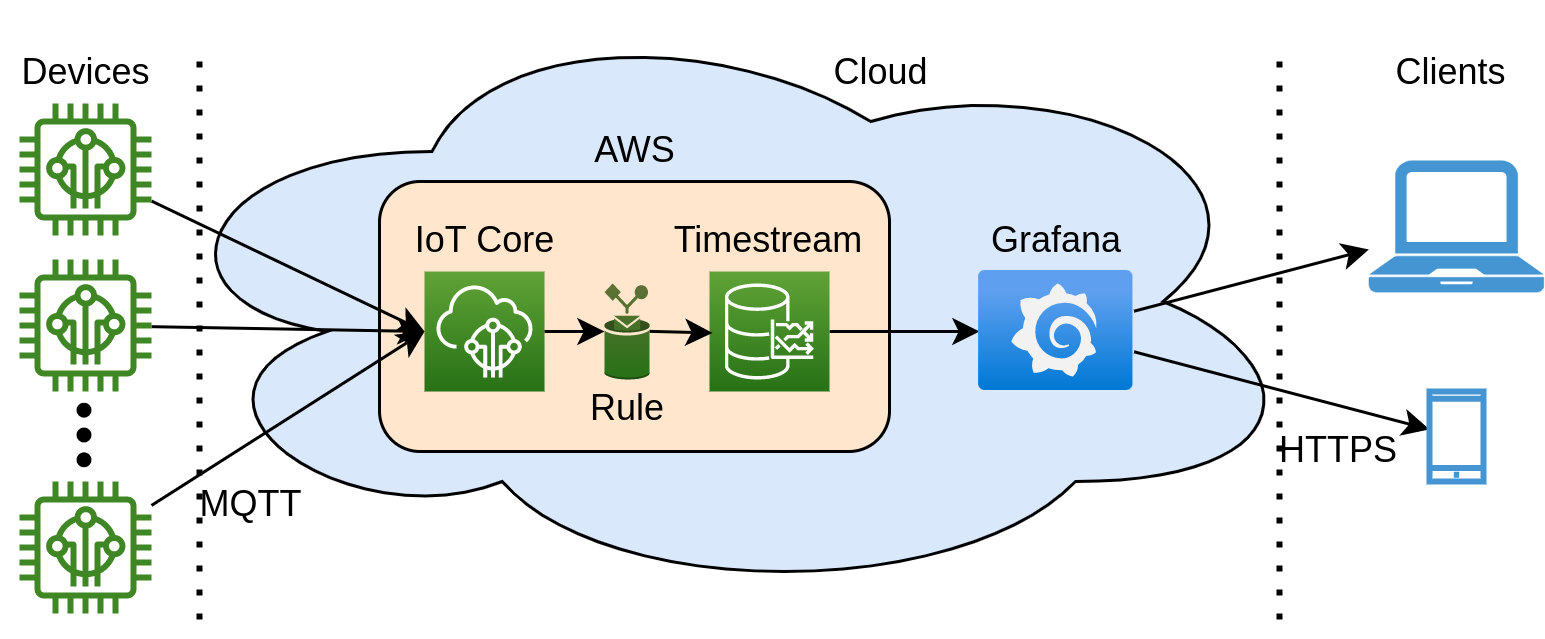
\includegraphics[scale=0.22]{./Figures/cc_diagram.png}
	\caption{Arquitectura de los servicios en la nube.}
	\label{fig:cc_diagram}
\end{figure}

\subsection{Gestión de dispositivos con IoT Core}
\label{subsection3_3_1}
\subsection{Bases de datos de series temporales con TimeStream}
\subsection{Visualiación de datos con Grafana}





% Chapter Template

\chapter{Ensayos y resultados} % Main chapter title
En este capítulo se presentan las pruebas realizadas sobre el prototipo de pruebas del sistema. Se detallan los procedimientos para probar los modelos para detección facial, el sensor de movimiento, el consumo energético del sistema y los servicios en la nube empleados.

\label{Chapter4} % Change X to a consecutive number; for referencing this chapter elsewhere, use \ref{ChapterX}

%----------------------------------------------------------------------------------------
% SECTION 1
%----------------------------------------------------------------------------------------
\section{Banco de pruebas}
Para llevar a cabo pruebas y mediciones precisas sobre el sistema, fue necesario montar un conjunto de herramientas e instrumentos para evaluar su funcionamiento. El banco de pruebas utilizado para este trabajo es el que se muestra en la figura \ref{fig:test_bench}.

\begin{figure}[h]
	\centering
	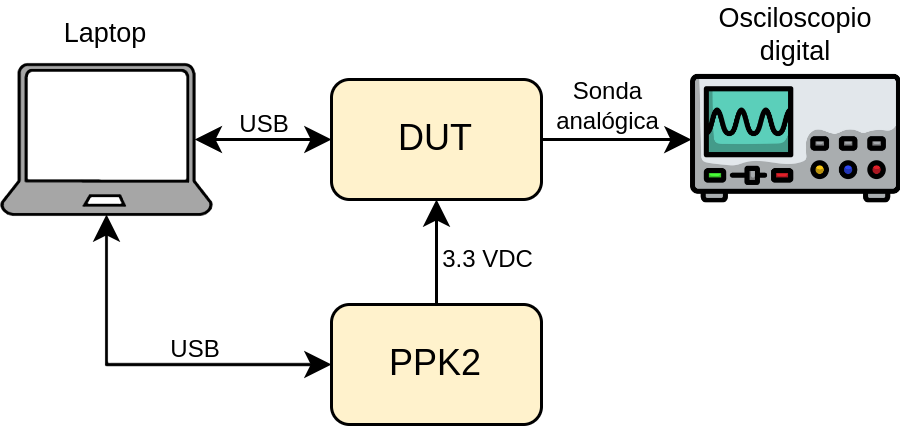
\includegraphics[scale=0.3]{./Figures/test_bench.png}
	\caption{Diagrama del banco de pruebas.}
	\label{fig:test_bench}
\end{figure}

Los componentes que conforman el banco de pruebas según la figura \ref{fig:test_bench} son:
\begin{itemize}
	\item Laptop: cumple la función de ejecutar el \textit{software} necesario para ejecutar las pruebas, monitorear y controlar todos los periféricos conectados mediante USB.
	\item Osciloscopio digital: TDS200C de Tektronix, es el instrumento utilizado para visualizar y medir las señales eléctricas generadas por el sistema. Su función principal para este trabajo fue evaluar las señales generadas por el sensor de movimiento.
	\item PPK2: Power Profiler Kit 2 de Texas Instruments, es un \textit{datalogger} enfocado en la medición de corrientes muy pequeñas y sirivió para evaluar el consumo de corriente del dispositivo.
	\item DUT: es el prototipo de pruebas en sí, sobre este se realizan todas las pruebas y mediciones con todos las herramientas del banco de pruebas.
\end{itemize}

%----------------------------------------------------------------------------------------
% SECTION 2
%----------------------------------------------------------------------------------------
\section{Pruebas sobre los modelos}
Estas pruebas tuvieron el objetivo de ensayar el \textit{pipeline} donde se encuentran los modelos de MTCNN para detección facial obtenidos para TensorFlow, TensorFlow Lite sin cuantización, TensorFlow Lite con cuantización a 8 bits y TensorFlow Lite Micro con cuantización a 8 bits. La figura \ref{fig:test_image} presenta una imagen que contiene tres rostros de formato RGB888 y dimensiones 96x96 píxeles, que fue utilizada como entrada para los \textit{pipelines} a probar.

\begin{figure}[h]
	\centering
	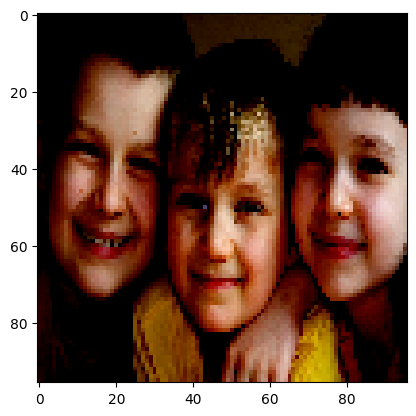
\includegraphics[scale=0.75]{./Figures/test_image.png}
	\caption{Imagen de prueba para los modelos.}
	\label{fig:test_image}
\end{figure}

Para probar los modelos para TensorFlow, TensorFlow Lite sin cuantización y TensorFlow Lite con cuantización a 8 bits, se utilizó Google Colab en conjunto con el \textit{framework} TensorFlow en lenguaje Python y algunas bibliotecas para visualización de imágenes. En las figuras \ref{fig:test_tf_pnet}, \ref{fig:test_tf_rnet} y \ref{fig:test_tf_onet} se muestran los resultados obtenidos.

\begin{figure}[!htpb]
     \centering
     \begin{subfigure}[b]{0.28\textwidth}
         \centering
         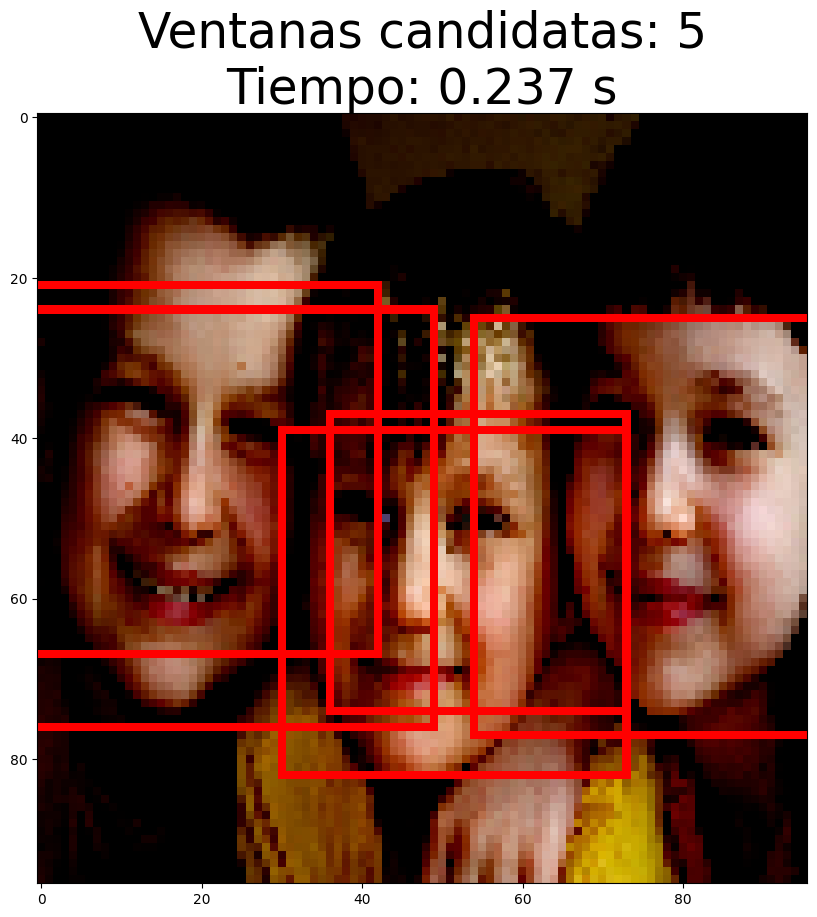
\includegraphics[width=\textwidth]{./Figures/test_tf_pnet_a.png}
         \caption{P-Net postprocesado.}
         \label{fig:1de3}
     \end{subfigure}
     \hfill
     \begin{subfigure}[b]{0.28\textwidth}
         \centering
         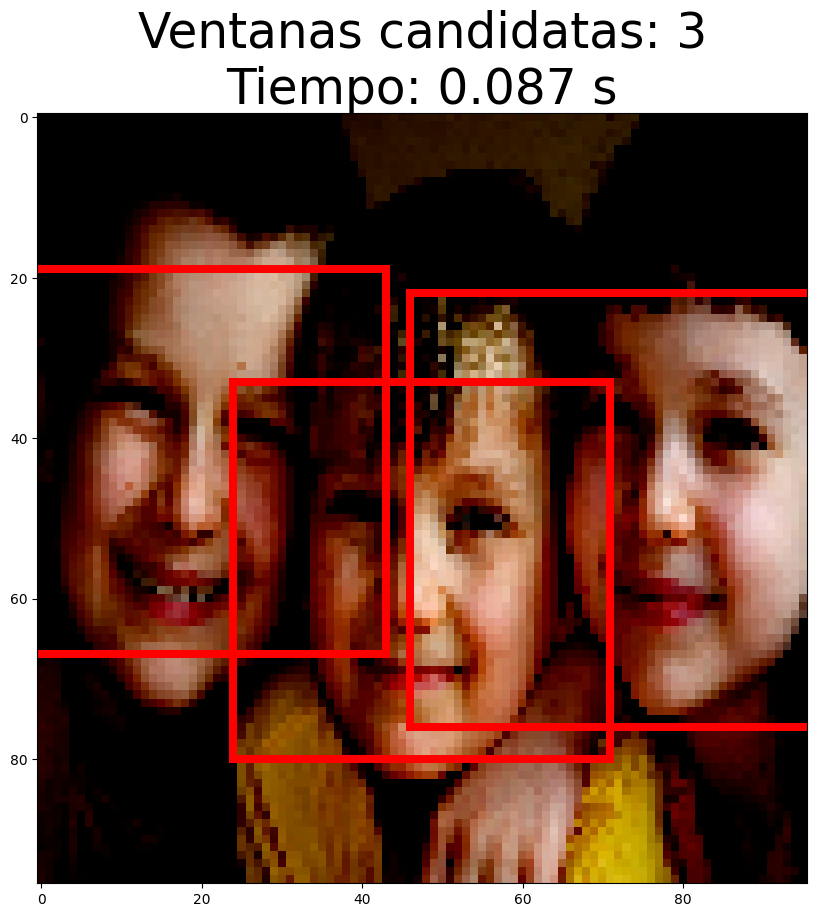
\includegraphics[width=\textwidth]{./Figures/test_tf_rnet_a.png}
         \caption{R-Net postprocesado.}
         \label{fig:2de3}
     \end{subfigure}
     \hfill
	 \begin{subfigure}[b]{0.28\textwidth}
         \centering
         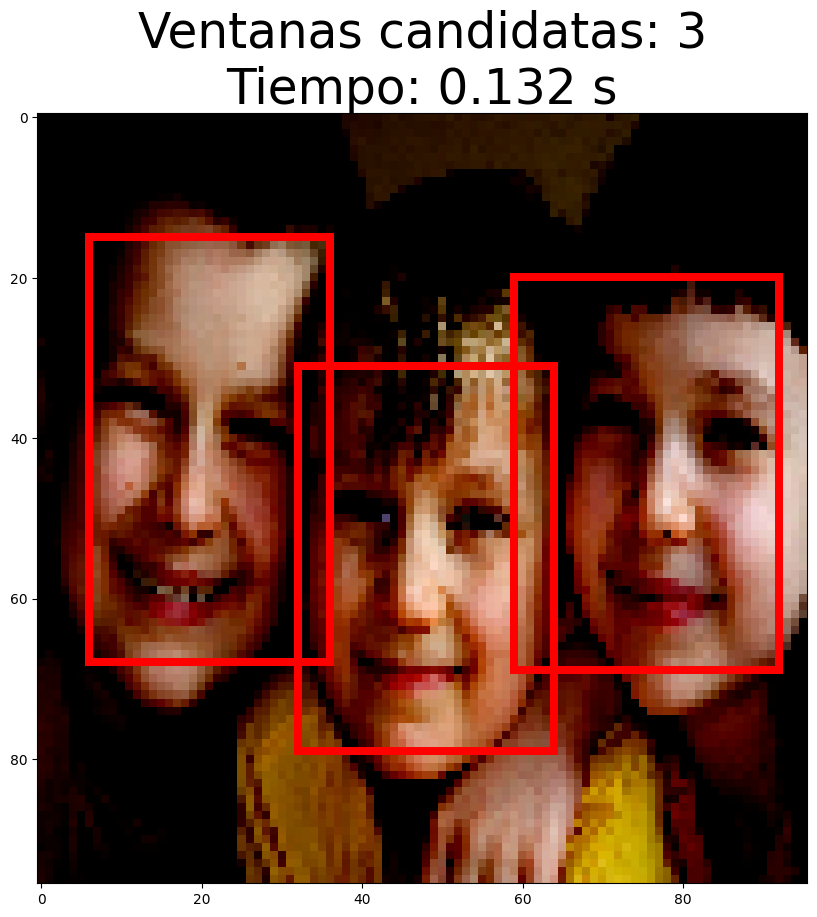
\includegraphics[width=\textwidth]{./Figures/test_tf_onet_a.png}
         \caption{O-Net postprocesado.}
         \label{fig:2de3}
     \end{subfigure}
     \hfill
        \caption{Resultados para TensorFlow.}
        \label{fig:test_tf_pnet}
\end{figure}

\clearpage


\begin{figure}[!htpb]
     \centering
     \begin{subfigure}[b]{0.28\textwidth}
         \centering
         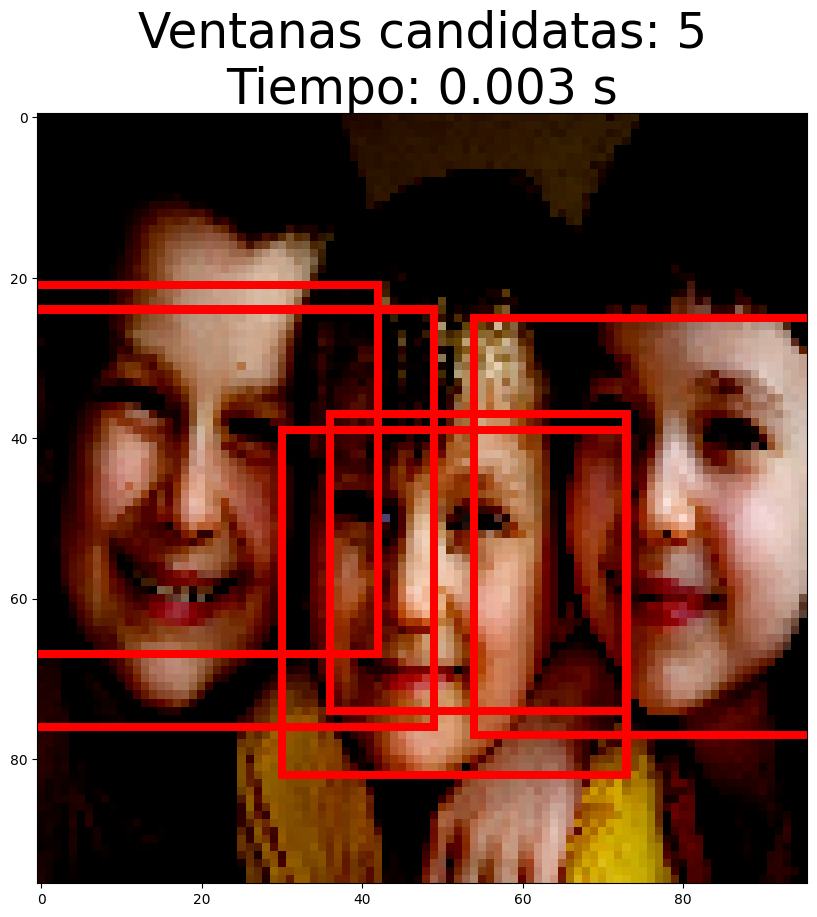
\includegraphics[width=\textwidth]{./Figures/test_tf_pnet_b.png}
         \caption{P-Net postprocesado.}
         \label{fig:1de3}
     \end{subfigure}
     \hfill
     \begin{subfigure}[b]{0.28\textwidth}
         \centering
         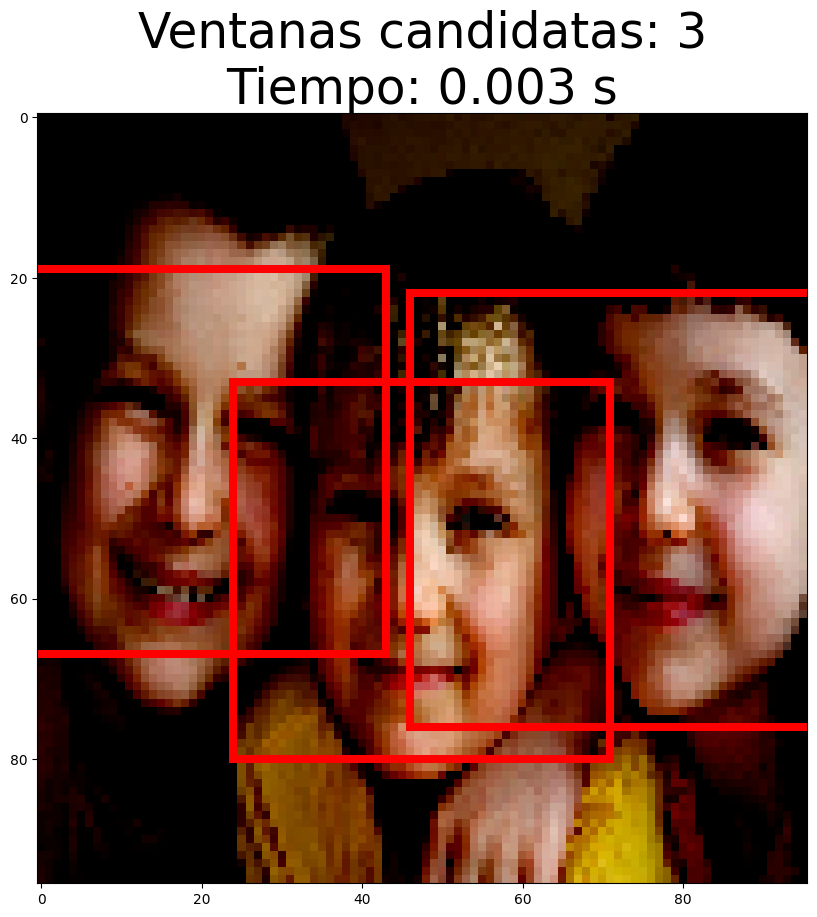
\includegraphics[width=\textwidth]{./Figures/test_tf_rnet_b.png}
         \caption{R-Net postprocesado.}
         \label{fig:2de3}
     \end{subfigure}
     \hfill
	 \begin{subfigure}[b]{0.28\textwidth}
         \centering
         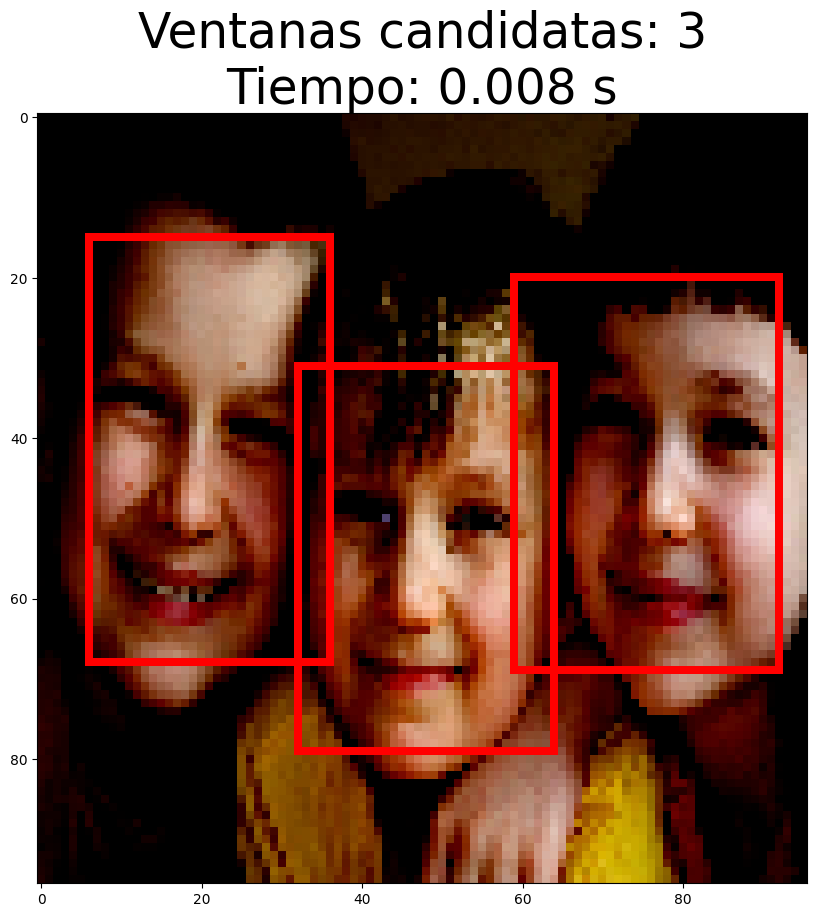
\includegraphics[width=\textwidth]{./Figures/test_tf_onet_b.png}
         \caption{O-Net postprocesado.}
         \label{fig:2de3}
     \end{subfigure}
     \hfill
        \caption{Resultados para TensorFlow Lite sin cuantización.}
        \label{fig:test_tf_rnet}
\end{figure}

\begin{figure}[!htpb]
     \centering
     \begin{subfigure}[b]{0.28\textwidth}
         \centering
         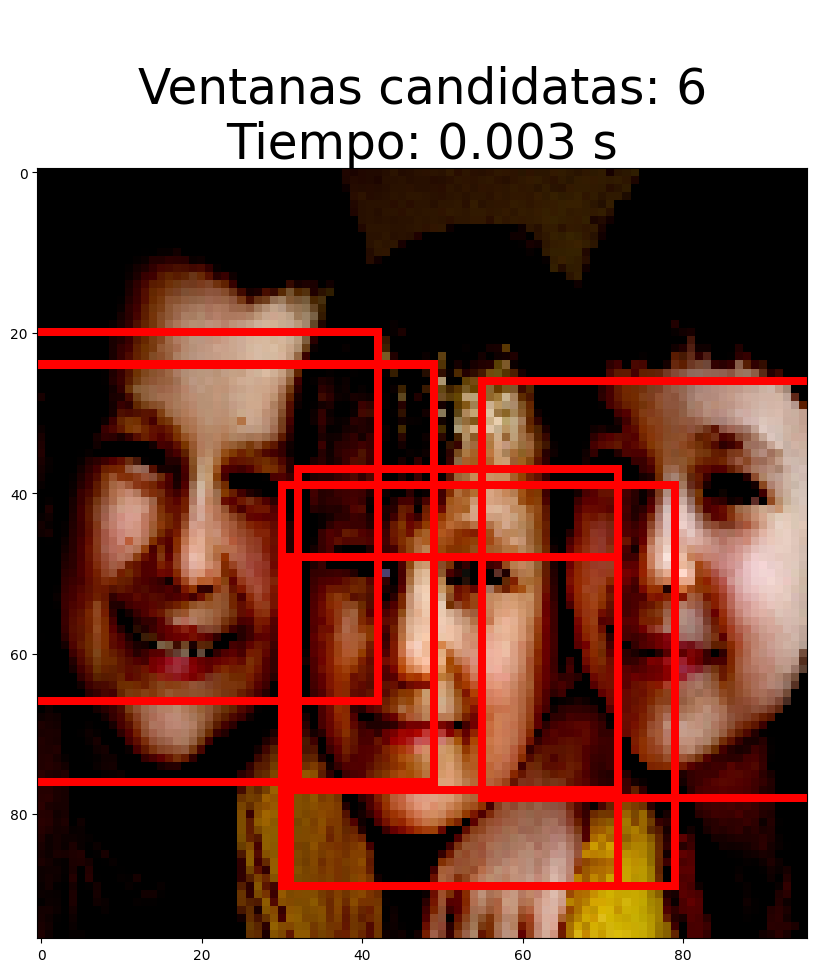
\includegraphics[width=\textwidth]{./Figures/test_tf_pnet_c.png}
         \caption{P-Net postprocesado.}
         \label{fig:1de3}
     \end{subfigure}
     \hfill
     \begin{subfigure}[b]{0.28\textwidth}
         \centering
         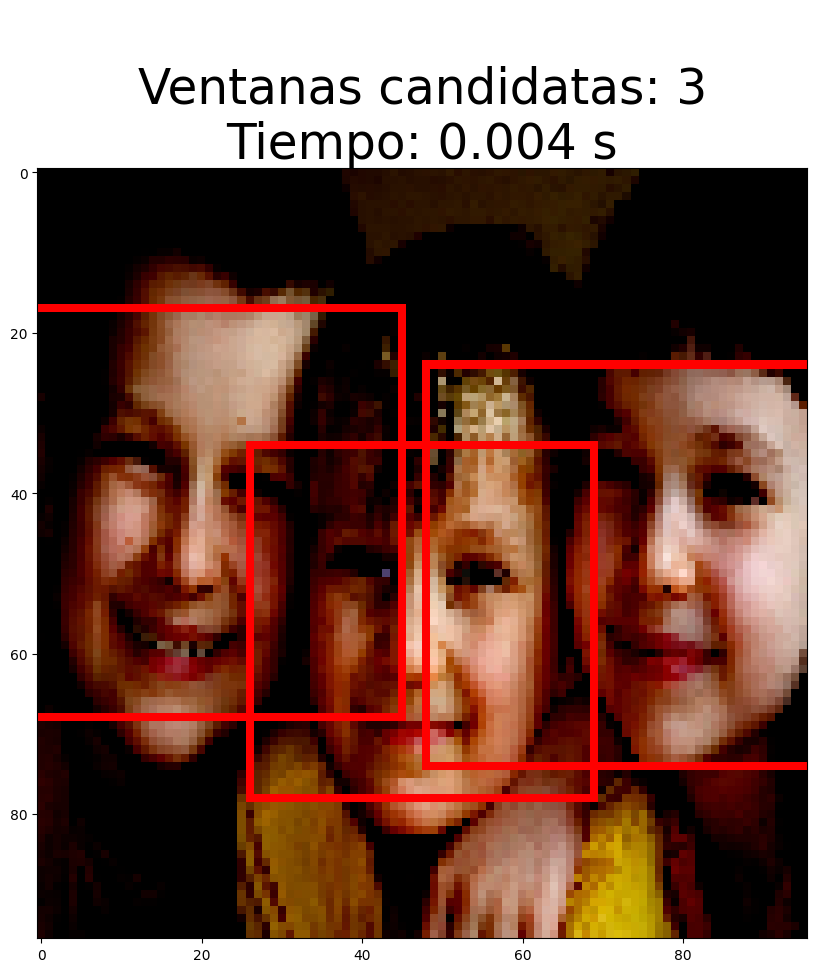
\includegraphics[width=\textwidth]{./Figures/test_tf_rnet_c.png}
         \caption{R-Net postprocesado.}
         \label{fig:2de3}
     \end{subfigure}
     \hfill
	 \begin{subfigure}[b]{0.28\textwidth}
         \centering
         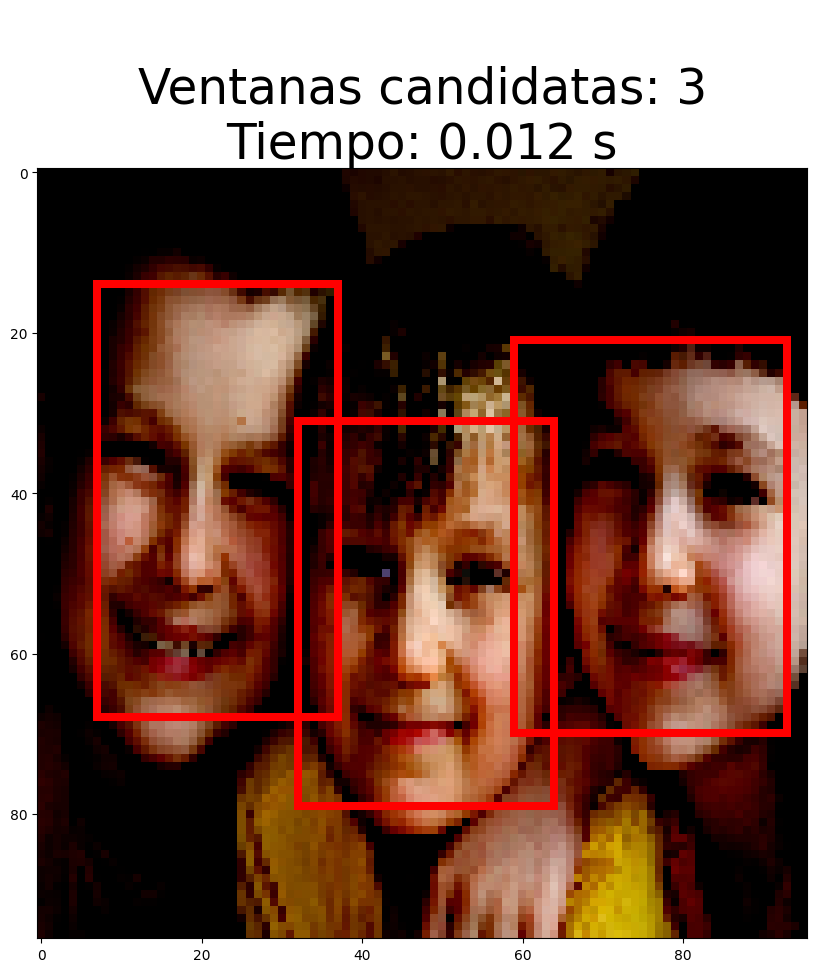
\includegraphics[width=\textwidth]{./Figures/test_tf_onet_c.png}
         \caption{O-Net postprocesado.}
         \label{fig:2de3}
     \end{subfigure}
     \hfill
        \caption{Resultados para TensorFlow Lite con cuantización a 8 bits.}
        \label{fig:test_tf_onet}
\end{figure}

Para probar el \textit{pipeline} y los modelos de MTCNN para TensorFlow Lite Micro con cuantización a 8 bits, se modificó el \textit{firmware} del prototipo de pruebas para que la imagen de prueba esté embebida en el binario de la aplicación y pueda ser leída dentro del programa. En la figura \ref{fig:test_tflm} se observan los resultados de esta prueba.

\begin{figure}[!htpb]
     \centering
     \begin{subfigure}[b]{0.28\textwidth}
         \centering
         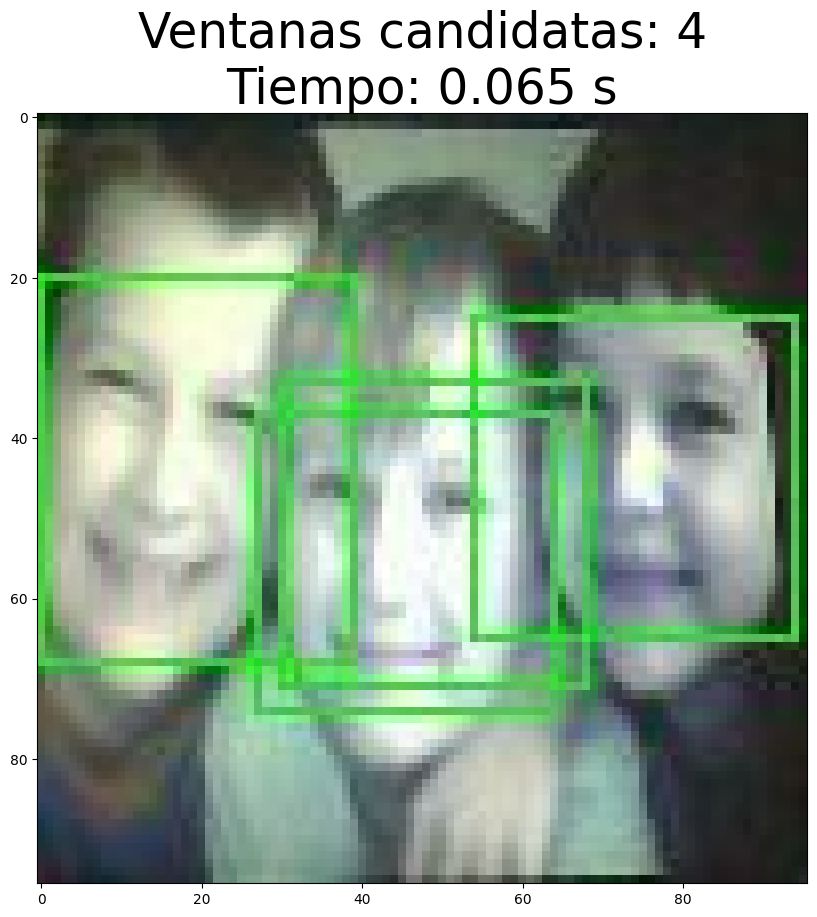
\includegraphics[width=\textwidth]{./Figures/pnet.png}
         \caption{P-Net postprocesado.}
         \label{fig:1de3}
     \end{subfigure}
     \hfill
     \begin{subfigure}[b]{0.28\textwidth}
         \centering
         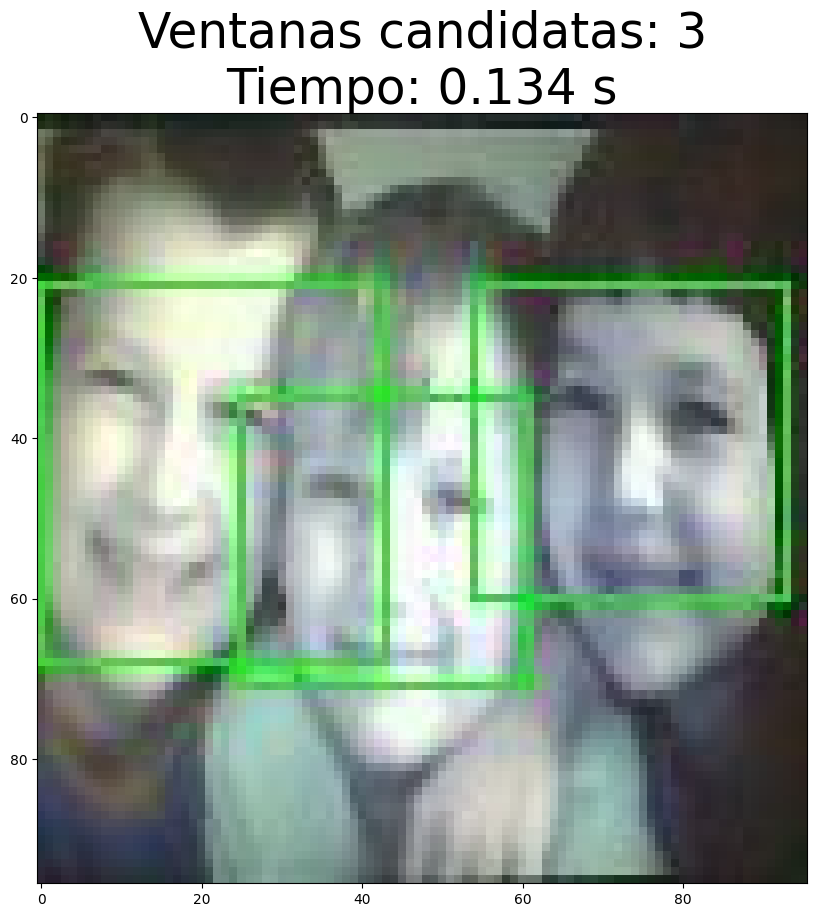
\includegraphics[width=\textwidth]{./Figures/rnet.png}
         \caption{R-Net postprocesado.}
         \label{fig:2de3}
     \end{subfigure}
     \hfill
	 \begin{subfigure}[b]{0.28\textwidth}
         \centering
         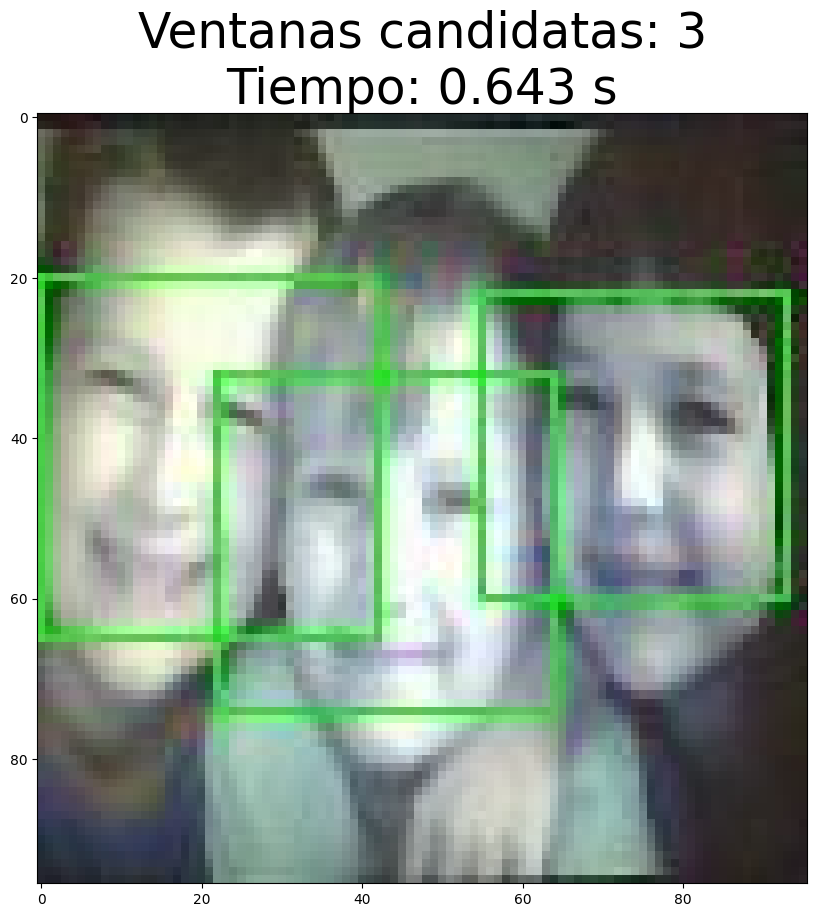
\includegraphics[width=\textwidth]{./Figures/onet.png}
         \caption{O-Net postprocesado.}
         \label{fig:2de3}
     \end{subfigure}
     \hfill
        \caption{Resultados para TensorFlow Lite Micro con cuantización a 8 bits.}
        \label{fig:test_tflm}
\end{figure}

Los resultados obtenidos de las pruebas en Google Colab fueron los esperados. A medida que los modelos se iban optimizando en tamaño y tiempo de respuesta, la precisión de los resultados se reducía. Para las pruebas realizadas sobre el prototipo de pruebas, los resultados también estuvieron acordes a lo planeado, si bien el tamaño es el más pequeño posible, los tiempos de inferencia son mucho más altos que para los modelos probados en Google Colab, debido a las limitaciones de hardware del ESP32-S3, aun así los resultados finales son muy similares. En la tabla \ref{tab:test_tf_models} se exponen los resultados para todas las pruebas sobre los modelos.

\begin{table}[h]
	\centering
	\caption[Resultados de las pruebas sobre los modelos]{Resultados de las pruebas sobre los modelos.}
	\begin{tabular}{lcc}   
		\toprule
		\textbf{Modelo} & \textbf{Rostros encontrados} & \textbf{Tiempo de ejecución MTCNN (ms)} \\
		\midrule
		TF & 3 & 456 \\
		TF Lite & 3 & 14 \\
		TF Lite 8 bits & 3 & 19 \\
		TF Lite Micro 8 bits & 3 & 842 \\
		\bottomrule
		\hline
	\end{tabular}
	\label{tab:test_tf_models}
\end{table}

%----------------------------------------------------------------------------------------
% SECTION 3
%----------------------------------------------------------------------------------------
\section{Pruebas sobre el sensor de movimiento}
Las pruebas realizadas sobre el sensor de movimiento tuvieron el objetivo de determinar el comportamiento de las señales de salida generadas por el TLV8544 cuando se genera movimiento en el rango de acción del sensor PIR. Para este fin se conectaron las sondas del osciloscopio en la salida de la señal analógica y en las 2 salidas digitales de los comparadores. En la figura \ref{fig:test_pir} se observan las señales capturadas por el osciloscopio para 5 movimientos detectados por el sensor PIR.

\begin{figure}[h]
	\centering
	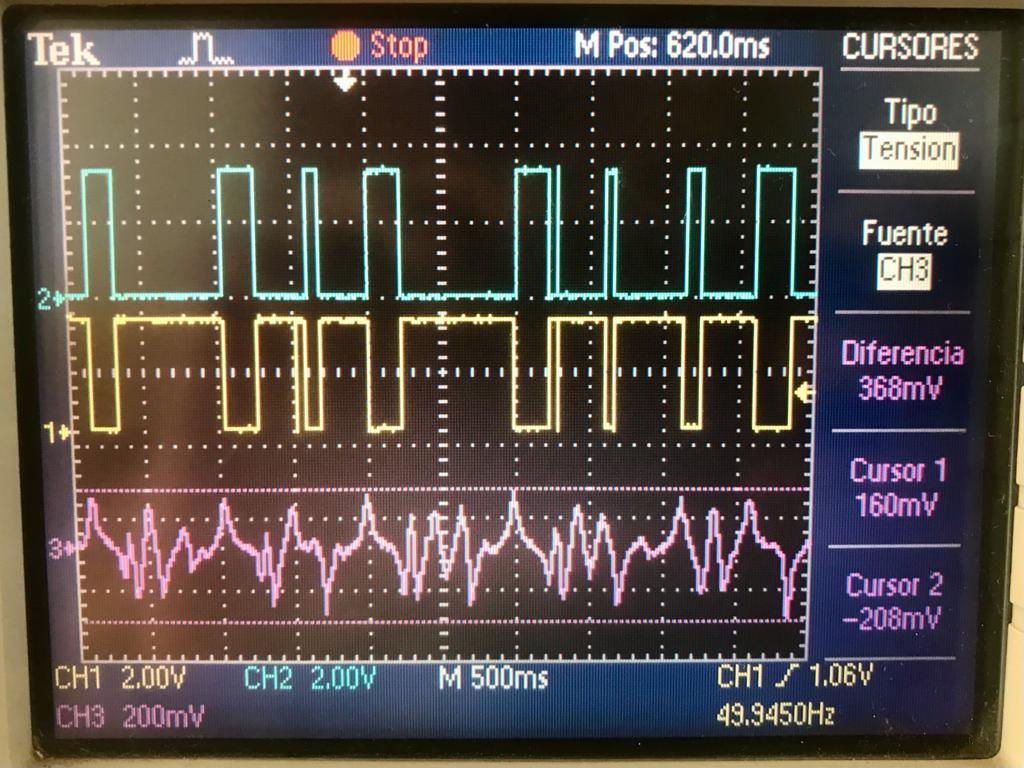
\includegraphics[scale=0.35]{./Figures/test_pir.jpeg}
	\caption{Señales de salida del sensor de movimiento.}
	\label{fig:test_pir}
\end{figure}

Como se puede observar de la figura \ref{fig:test_pir} se generaron señales de corta duración que causaron falsos positivos en la detección de movimiento. Este efecto fue subsanado con la ayuda de una máquina de estados implementada en el programa que corre el coprocesador ULP.

%----------------------------------------------------------------------------------------
% SECTION 4
%----------------------------------------------------------------------------------------
\section{Pruebas de consumo energético sobre el sistema}
Estas pruebas consistieron en poner en funcionamiento el prototipo de pruebas y medir el consumo de corriente para determinar si todas las técnicas de bajo consumo fueron aplicadas correctamente. Como se mostró en la figura \ref{fig:ulp_modes} el sistema durante su funcionamiento realiza transiciones entre 3 estados distintos, donde cada estado tiene un consumo de corriente diferente. Con ayuda del PPK2 y del software nRF Connect for Desktop con su módulo Power Profile, se midió el consumo de corriente del sistema durante un tiempo de 5 minutos, donde fue activado en varias ocasiones mediante el sensor de movimiento. En la figura \ref{fig:test_ulp2} se observa un gráfico donde se puede apreciar el comportamiento del sistema a través del cambio de la forma de la corriente de consumo con relación al tiempo.

\begin{figure}[h]
	\centering
	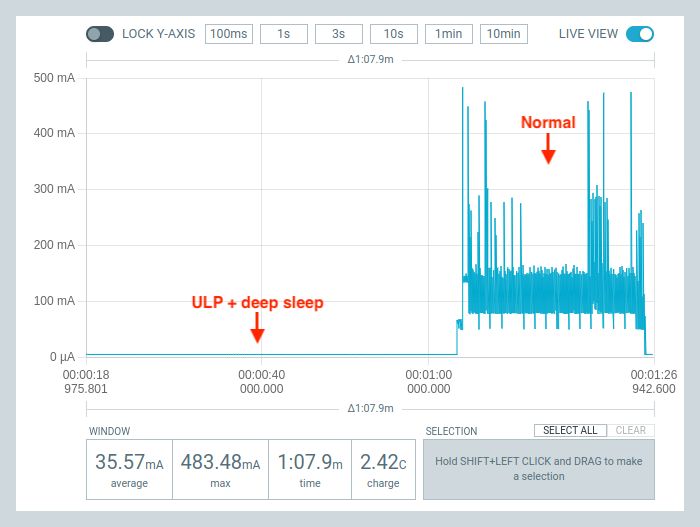
\includegraphics[scale=0.45]{./Figures/test_ulp1.png}
	\caption{Gráfico de consumo de corriente para un ciclo de funcionamiento.}
	\label{fig:test_ulp1}
\end{figure}

La figura \ref{fig:test_ulp1} muestra un funcionamiento normal del dipositivo, es decir, que se mantiene entre los modos ULP y \textit{deep sleep} hasta que detecta un movimiento válido mediante el sensor de movimiento y activa el procesador principal para realizar las tareas de detección facial y comunicación con los servicios en la nube. La transición entre los estados \textit{deep sleep} y ULP sucede cada 100 ms, como se muestra en la figura \ref{fig:test_ulp2}, donde en el estado ULP se ejecuta la máquina de estados que mitiga los errores causados por los falsos positivos generados por el sensor de movimiento.

\clearpage


\begin{figure}[h]
	\centering
	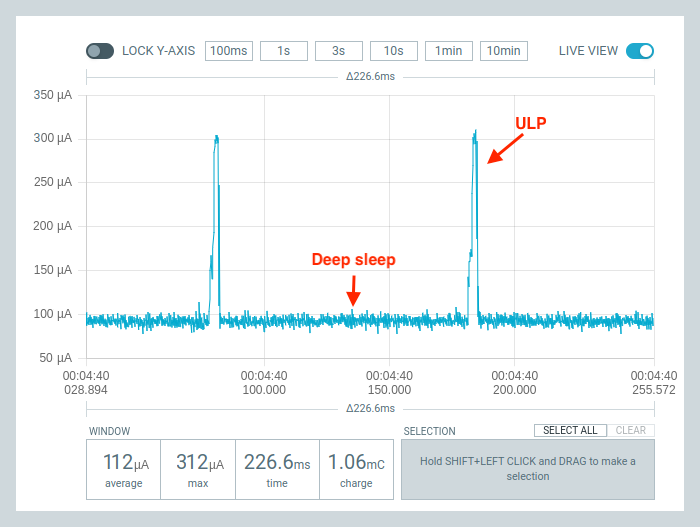
\includegraphics[scale=0.45]{./Figures/test_ulp2.png}
	\caption{Gráfico de consumo de corriente en modo de bajo consumo.}
	\label{fig:test_ulp2}
\end{figure}

En la tabla \ref{tab:test_ulp} se detallan los consumos de corriente y los tiempos de duración de todos los estados de consumo del dispositivo.

\begin{table}[h]
	\centering
	\caption[Consumo de corriente del dispositivo]{Consumo de corriente aproximado de todos los modos del dispositivo.}
	\begin{tabular}{lccc}   
		\toprule
		\textbf{Estado} & \textbf{Consumo promedio (mA)} & \textbf{Consumo máximo (mA)} & \textbf{Tiempo (s)} \\
		\midrule
		Normal & 97,31 & 478,21 & 22,8 \\
		ULP & 0,247 & 0,310 & 0,003 \\
		\textit{Deep sleep} & 0,112 & 0,121 & 0,1 \\
		\bottomrule
		\hline
	\end{tabular}
	\label{tab:test_ulp}
\end{table}

El evento que despierta al procesador principal para ejecutar las tareas de detección facial y comunicación con los servicios en la nube es asíncrono, es decir, que no es posible predecirlo, por lo que no fue posible medir una corriente promedio del dispositivo en general y por tanto tampoco se pudo establecer el tiempo que un par de baterías de litio AA podría alimentar el dispositivo.

%----------------------------------------------------------------------------------------
% SECTION 5
%----------------------------------------------------------------------------------------
\section{Pruebas sobre los servicios en la nube}
Las pruebas sobre los servicios en la nube se basaron en simular la conexión y publicación de mensajes de tres dispositivos distintos por un lapso de 10 minutos. La simulación de los dispositivos se hizo con ayuda del \textit{script} de Python mostrado en \ref{cod:test_iot}, que tiene la función de conectarse al broker de Iot Core y publicar 15 mensajes en un lapso de 15 minutos para cada uno de los dispositivos a simular.

\begin{lstlisting}[language=Python, label=cod:test_iot, caption=Código del \textit{script} para probar IoT Core.]
from random import random
from awscrt import mqtt
from awsiot import mqtt_connection_builder
import time as t
import random

ENDPOINT = "xxxxxxxxxxxxxxxxxxxxxxxxxxxxxxx.amazonaws.com"
CLIENT_ID = "dev1"
PATH_TO_CERTIFICATE = "dev_cert.pem.crt"
PATH_TO_PRIVATE_KEY = "priv_key.pem.key"
PATH_TO_AMAZON_ROOT_CA_1 = "AmazonRootCA1.pem"
TOPIC = "faceCounter"

mqtt_connection = mqtt_connection_builder.mtls_from_path(endpoint=ENDPOINT, cert_filepath=PATH_TO_CERTIFICATE, pri_key_filepath=PATH_TO_PRIVATE_KEY, ca_filepath=PATH_TO_AMAZON_ROOT_CA_1, client_id=CLIENT_ID, clean_session=False, keep_alive_secs=6)

# Device IDs
id = ["7a5b4c79-621d-476d-83b4-861005589752", "8a5b4c79-621d-476d-83b4-861005589752", "9a5b4c79-621d-476d-83b4-861005589752"]

# Connect to broker
connect_future = mqtt_connection.connect()
connect_future.result()

# Send messages for all IDs
for i in range(30):
    for j in id:
        # Set new values for the JSON message
        message = "{\n\"id\":\"%s\",\n\"payload\":{\n\"faces\":%d,\n\"battery\":%d,\n\"temperature\":%d\n}\n}" % (j, random.randint(0, 5), random.randint(50, 90), random.randint(19, 27))
        mqtt_connection.publish(topic=TOPIC, payload=message, qos=mqtt.QoS.AT_LEAST_ONCE)
    # Wait for 1 min
    t.sleep(60)

# Disconnect from broker
disconnect_future = mqtt_connection.disconnect()
disconnect_future.result()
\end{lstlisting}

Para controlar los mensajes que son recibidos por el \textit{broker} se utilizó el monitor MQTT de IoT Core MQTT Test, que consiste en un cliente que puede publicar y suscribirse a uno o varios tópicos. En la figura \ref{fig:test_iot} se observa un mensaje publicado por el \textit{script} del código \ref{cod:test_iot} en el tópico \texttt{faceCounter}.

\begin{figure}[h]
	\centering
	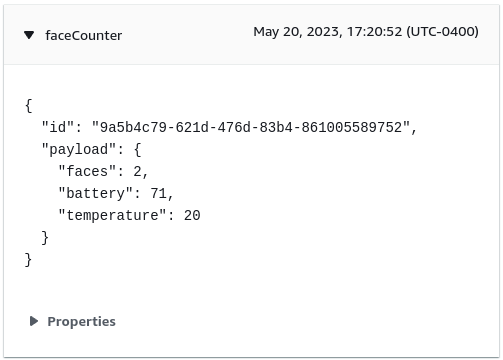
\includegraphics[scale=0.45]{./Figures/test_iot.png}
	\caption{Mensaje de prueba recibido en MQTT Test Client.}
	\label{fig:test_iot}
\end{figure}

Los mensajes publicados en \texttt{faceCounter} fueron procesados mediante un \textit{rule} para grabar los datos de relevancia en la tabla \texttt{faceCounter} de la base de datos \texttt{iot} de Timestream. El código \ref{cod:test_sql} consulta los datos de los últimos 5 minutos de  de la tabla \texttt{faceCounter} y en la figura \ref{fig:test_timestream} se muestran los resultados obtenidos.

\begin{lstlisting}[language=SQL, label=cod:test_sql, caption=Código SQL para obtener los datos de la tabla faceCounter.]
SELECT * FROM "iot"."faceCounter" WHERE time between ago(5m) and now() ORDER BY time 
\end{lstlisting}

\begin{figure}[h]
	\centering
	\includegraphics[scale=0.45]{./Figures/test_timestream.png}
	\caption{Tabla faceCounter con los datos de prueba.}
	\label{fig:test_timestream}
\end{figure}

Finalmente, en la figura \ref{fig:test_dashboard} se exhibe el \textit{dashboard} creado con Grafana, donde cada columna representa mediante gráficos los datos de uno de los dispositivos simulados.
\begin{figure}[h]
	\centering
	\includegraphics[scale=0.3]{./Figures/test_dashboard.png}
	\caption{\textit{Dashboard} con datos de prueba para 3 dispositivos.}
	\label{fig:test_dashboard}
\end{figure}
 
% Chapter Template

\chapter{Conclusiones} % Main chapter title

\label{Chapter5} % Change X to a consecutive number; for referencing this chapter elsewhere, use \ref{ChapterX}


%----------------------------------------------------------------------------------------

%----------------------------------------------------------------------------------------
%	SECTION 1
%----------------------------------------------------------------------------------------

\section{Conclusiones generales }

La idea de esta sección es resaltar cuáles son los principales aportes del trabajo realizado y cómo se podría continuar. Debe ser especialmente breve y concisa. Es buena idea usar un listado para enumerar los logros obtenidos.

Algunas preguntas que pueden servir para completar este capítulo:

\begin{itemize}
\item ¿Cuál es el grado de cumplimiento de los requerimientos?
\item ¿Cuán fielmente se puedo seguir la planificación original (cronograma incluido)?
\item ¿Se manifestó algunos de los riesgos identificados en la planificación? ¿Fue efectivo el plan de mitigación? ¿Se debió aplicar alguna otra acción no contemplada previamente?
\item Si se debieron hacer modificaciones a lo planificado ¿Cuáles fueron las causas y los efectos?
\item ¿Qué técnicas resultaron útiles para el desarrollo del proyecto y cuáles no tanto?
\end{itemize}


%----------------------------------------------------------------------------------------
%	SECTION 2
%----------------------------------------------------------------------------------------
\section{Próximos pasos}
Esta memoria describe el proceso de diseño e implementación del prototipo de pruebas, que fue utilizado para comprobar la factibiliad técnica de todos los requerimientos funcionales planteados. Los proximos pasos de este trabajo tienen el objetivo de lograr un prototipo lo mas cercano posible a un dipositivo final que pueda ser comercializado, estos son:

\begin{enumerate}
	\item Incorporar componentes de hardware para controlar y monitorear el suministro de energía de las baterías.
	\item Diseñar el diagrama esquematico
	\item Seleccionar una carcasa adecuada al tamaño y entorno de aplicacion del dispositivo
	\item Diseñar un PCB cuyas dimensiones se correspondan con las de la carcasa.
	\item Implementar \textit{flash encryption},y \textit{secure boot} en el ESP32-S3 para mejorar la seguridad del dispositivo.
	\item Estudiar la factibilidad de utilziar FaceNet en el dispositivo para lograr que en conjunto con MTCNN realicen reconocimiento facial.
	\item Estudiar la factibilidad de utilizar Amazon Rekognition para realizar reconocimiento facial en la nube.
\end{enumerate}
 

%----------------------------------------------------------------------------------------
%	CONTENIDO DE LA MEMORIA  - APÉNDICES
%----------------------------------------------------------------------------------------

\appendix % indicativo para indicarle a LaTeX los siguientes "capítulos" son apéndices

% Incluir los apéndices de la memoria como archivos separadas desde la carpeta Appendices
% Descomentar las líneas a medida que se escriben los apéndices

%% Appendix A

\chapter{Appendix Title Here} % Main appendix title

\label{AppendixA} % For referencing this appendix elsewhere, use \ref{AppendixA}

Write your Appendix content here.
%\include{Appendices/AppendixB}
%\include{Appendices/AppendixC}

%----------------------------------------------------------------------------------------
%	BIBLIOGRAPHY
%----------------------------------------------------------------------------------------

\Urlmuskip=0mu plus 1mu\relax
\raggedright
\printbibliography[heading=bibintoc]

%----------------------------------------------------------------------------------------

\end{document}  
